\documentclass[journal]{IEEEtran}
\usepackage[utf8]{inputenc}
\usepackage[T1]{fontenc}
\usepackage{amsmath,amssymb,amsthm}
\usepackage{booktabs}
\usepackage{graphicx}
\usepackage{xcolor}
\usepackage{etoolbox}
\usepackage{multirow}
\usepackage{url}
\usepackage{tikz}
\usetikzlibrary{arrows.meta,positioning,fit,calc,shapes.geometric,backgrounds}
\usepackage[hidelinks]{hyperref}
\hypersetup{pdftitle={Every Round Is a Release: Communication-Budgeted Federated Learning Over Constrained Links}, pdfauthor={Abraheem Rashid}}
\usepackage{cite}

% ---------------------------------------------------------------------------
% Every number in this manuscript comes from paper/generated/, which
% src/analysis/collect.py writes from the per-seed logs. Nothing is typed by hand.
% A table whose runs do not exist renders [RUN REQUIRED].
% ---------------------------------------------------------------------------
\IfFileExists{generated/numbers.tex}{\newcommand{\TotalRuns}{2218}
\newcommand{\diabetesmlpFedavgAuroc}{0.6203}
\newcommand{\diabetesmlpFedavgAuprc}{0.171}
\newcommand{\diabetesmlpFedavgUploadMb}{218.4}
\newcommand{\diabetesmlpFedavgSeeds}{10}
\newcommand{\diabetesmlpFedavgVsFedperDiff}{-0.0012}
\newcommand{\diabetesmlpFedavgNiAurocP}{\ensuremath{<10^{-4}}}
\newcommand{\diabetesmlpFedavgNiAuprcP}{\ensuremath{<10^{-4}}}
\newcommand{\diabetesmlpFedavgUploadSavingPct}{-0}
\newcommand{\diabetesmlpFedproxAuroc}{0.6279}
\newcommand{\diabetesmlpFedproxAuprc}{0.175}
\newcommand{\diabetesmlpFedproxUploadMb}{218.4}
\newcommand{\diabetesmlpFedproxSeeds}{10}
\newcommand{\diabetesmlpFedproxVsFedperDiff}{+0.0065}
\newcommand{\diabetesmlpFedproxNiAurocP}{\ensuremath{<10^{-4}}}
\newcommand{\diabetesmlpFedproxNiAuprcP}{\ensuremath{<10^{-4}}}
\newcommand{\diabetesmlpFedproxUploadSavingPct}{-0}
\newcommand{\diabetesmlpScaffoldAuroc}{0.5930}
\newcommand{\diabetesmlpScaffoldAuprc}{0.138}
\newcommand{\diabetesmlpScaffoldUploadMb}{436.9}
\newcommand{\diabetesmlpScaffoldSeeds}{10}
\newcommand{\diabetesmlpScaffoldVsFedperDiff}{-0.0284}
\newcommand{\diabetesmlpScaffoldNiAurocP}{=0.997}
\newcommand{\diabetesmlpScaffoldNiAuprcP}{=1.000}
\newcommand{\diabetesmlpScaffoldUploadSavingPct}{-101}
\newcommand{\diabetesmlpFedperAuroc}{0.6215}
\newcommand{\diabetesmlpFedperAuprc}{0.171}
\newcommand{\diabetesmlpFedperUploadMb}{217.8}
\newcommand{\diabetesmlpFedperSeeds}{10}
\newcommand{\diabetesmlpFedlamaAuroc}{0.6291}
\newcommand{\diabetesmlpFedlamaAuprc}{0.176}
\newcommand{\diabetesmlpFedlamaUploadMb}{154.1}
\newcommand{\diabetesmlpFedlamaSeeds}{10}
\newcommand{\diabetesmlpFedlamaVsFedperDiff}{+0.0076}
\newcommand{\diabetesmlpFedlamaNiAurocP}{\ensuremath{<10^{-4}}}
\newcommand{\diabetesmlpFedlamaNiAuprcP}{\ensuremath{<10^{-4}}}
\newcommand{\diabetesmlpFedlamaUploadSavingPct}{29}
\newcommand{\diabetesmlpAdacommAuroc}{0.6302}
\newcommand{\diabetesmlpAdacommAuprc}{0.168}
\newcommand{\diabetesmlpAdacommUploadMb}{29.1}
\newcommand{\diabetesmlpAdacommSeeds}{10}
\newcommand{\diabetesmlpAdacommVsFedperDiff}{+0.0087}
\newcommand{\diabetesmlpAdacommNiAurocP}{\ensuremath{<10^{-4}}}
\newcommand{\diabetesmlpAdacommNiAuprcP}{\ensuremath{<0.001}}
\newcommand{\diabetesmlpAdacommUploadSavingPct}{87}
\newcommand{\diabetesmlpLagAuroc}{0.6351}
\newcommand{\diabetesmlpLagAuprc}{0.179}
\newcommand{\diabetesmlpLagUploadMb}{218.4}
\newcommand{\diabetesmlpLagSeeds}{10}
\newcommand{\diabetesmlpLagVsFedperDiff}{+0.0136}
\newcommand{\diabetesmlpLagNiAurocP}{\ensuremath{<10^{-4}}}
\newcommand{\diabetesmlpLagNiAuprcP}{\ensuremath{<10^{-4}}}
\newcommand{\diabetesmlpLagUploadSavingPct}{-0}
\newcommand{\diabetesmlpFixedAuroc}{0.6339}
\newcommand{\diabetesmlpFixedAuprc}{0.177}
\newcommand{\diabetesmlpFixedUploadMb}{82.9}
\newcommand{\diabetesmlpFixedSeeds}{10}
\newcommand{\diabetesmlpFixedVsFedperDiff}{+0.0124}
\newcommand{\diabetesmlpFixedNiAurocP}{\ensuremath{<10^{-4}}}
\newcommand{\diabetesmlpFixedNiAuprcP}{\ensuremath{<10^{-4}}}
\newcommand{\diabetesmlpFixedUploadSavingPct}{62}
\newcommand{\diabetesmlpTierfedAuroc}{0.6269}
\newcommand{\diabetesmlpTierfedAuprc}{0.175}
\newcommand{\diabetesmlpTierfedUploadMb}{65.3}
\newcommand{\diabetesmlpTierfedSeeds}{10}
\newcommand{\diabetesmlpTierfedVsFedperDiff}{+0.0054}
\newcommand{\diabetesmlpTierfedNiAurocP}{\ensuremath{<10^{-4}}}
\newcommand{\diabetesmlpTierfedNiAuprcP}{\ensuremath{<10^{-4}}}
\newcommand{\diabetesmlpTierfedUploadSavingPct}{70}
\newcommand{\diabetesmlpNTrain}{55,992}
\newcommand{\diabetesmlpNTest}{13,998}
\newcommand{\diabetesmlpNFeatures}{160}
\newcommand{\diabetesmlpNPatients}{55,992}
\newcommand{\diabetesmlpPrevalence}{9.0}
\newcommand{\diabetesmlpPrevalenceFrac}{0.09}
\newcommand{\diabetesmlpMaxClientShare}{12}
\newcommand{\diabetesmlpLabelTv}{0.009}
\newcommand{\diabetesmlpTierSlowParams}{20,608}
\newcommand{\diabetesmlpTierSlowPct}{45.3}
\newcommand{\diabetesmlpTierMediumParams}{24,768}
\newcommand{\diabetesmlpTierMediumPct}{54.4}
\newcommand{\diabetesmlpTierFastParams}{130}
\newcommand{\diabetesmlpTierFastPct}{0.3}
\newcommand{\diabetesmlpTierTotalParams}{45,506}
\newcommand{\diabetesmlpTierTotalPct}{100.0}
\newcommand{\medmnistcnnFedavgAuroc}{0.9959}
\newcommand{\medmnistcnnFedavgAuprc}{0.991}
\newcommand{\medmnistcnnFedavgUploadMb}{1214.8}
\newcommand{\medmnistcnnFedavgSeeds}{10}
\newcommand{\medmnistcnnFedavgVsFedperDiff}{+0.0316}
\newcommand{\medmnistcnnFedavgNiAurocP}{=0.037}
\newcommand{\medmnistcnnFedavgNiAuprcP}{\ensuremath{<0.001}}
\newcommand{\medmnistcnnFedavgUploadSavingPct}{-0}
\newcommand{\medmnistcnnFedperAuroc}{0.9643}
\newcommand{\medmnistcnnFedperAuprc}{0.986}
\newcommand{\medmnistcnnFedperUploadMb}{1213.7}
\newcommand{\medmnistcnnFedperSeeds}{10}
\newcommand{\medmnistcnnFedlamaAuroc}{0.9965}
\newcommand{\medmnistcnnFedlamaAuprc}{0.995}
\newcommand{\medmnistcnnFedlamaUploadMb}{877.4}
\newcommand{\medmnistcnnFedlamaSeeds}{10}
\newcommand{\medmnistcnnFedlamaVsFedperDiff}{+0.0322}
\newcommand{\medmnistcnnFedlamaNiAurocP}{=0.036}
\newcommand{\medmnistcnnFedlamaNiAuprcP}{=0.005}
\newcommand{\medmnistcnnFedlamaUploadSavingPct}{28}
\newcommand{\medmnistcnnFixedAuroc}{0.9642}
\newcommand{\medmnistcnnFixedAuprc}{0.989}
\newcommand{\medmnistcnnFixedUploadMb}{614.8}
\newcommand{\medmnistcnnFixedSeeds}{10}
\newcommand{\medmnistcnnFixedVsFedperDiff}{-0.0001}
\newcommand{\medmnistcnnFixedNiAurocP}{\ensuremath{<10^{-4}}}
\newcommand{\medmnistcnnFixedNiAuprcP}{=0.002}
\newcommand{\medmnistcnnFixedUploadSavingPct}{49}
\newcommand{\medmnistcnnTierfedAuroc}{0.9698}
\newcommand{\medmnistcnnTierfedAuprc}{0.984}
\newcommand{\medmnistcnnTierfedUploadMb}{364.1}
\newcommand{\medmnistcnnTierfedSeeds}{10}
\newcommand{\medmnistcnnTierfedVsFedperDiff}{+0.0055}
\newcommand{\medmnistcnnTierfedNiAurocP}{=0.182}
\newcommand{\medmnistcnnTierfedNiAuprcP}{=0.090}
\newcommand{\medmnistcnnTierfedUploadSavingPct}{70}
\newcommand{\medmnistcnnNTrain}{5,232}
\newcommand{\medmnistcnnNTest}{624}
\newcommand{\medmnistcnnNFeatures}{784}
\newcommand{\medmnistcnnNPatients}{5,232}
\newcommand{\medmnistcnnPrevalence}{74.2}
\newcommand{\medmnistcnnPrevalenceFrac}{0.74}
\newcommand{\medmnistcnnMaxClientShare}{14}
\newcommand{\medmnistcnnLabelTv}{0.370}
\newcommand{\medmnistcnnTierSlowParams}{9,696}
\newcommand{\medmnistcnnTierSlowPct}{3.4}
\newcommand{\medmnistcnnTierMediumParams}{277,632}
\newcommand{\medmnistcnnTierMediumPct}{96.5}
\newcommand{\medmnistcnnTierFastParams}{258}
\newcommand{\medmnistcnnTierFastPct}{0.1}
\newcommand{\medmnistcnnTierTotalParams}{287,586}
\newcommand{\medmnistcnnTierTotalPct}{100.0}
\newcommand{\dpAdacommSigmaFourAuroc}{0.5460}
\newcommand{\dpAdacommSigmaFourAuprc}{0.108}
\newcommand{\dpAdacommSigmaFourUploadMb}{29.1}
\newcommand{\dpAdacommSigmaFourTxRounds}{8}
\newcommand{\dpAdacommSigmaFourSeeds}{10}
\newcommand{\dpAdacommSigmaFourEps}{3.6}
\newcommand{\dpAdacommSigmaHalfAuroc}{0.6223}
\newcommand{\dpAdacommSigmaHalfAuprc}{0.158}
\newcommand{\dpAdacommSigmaHalfUploadMb}{29.1}
\newcommand{\dpAdacommSigmaHalfTxRounds}{8}
\newcommand{\dpAdacommSigmaHalfSeeds}{10}
\newcommand{\dpAdacommSigmaHalfEps}{43.2}
\newcommand{\dpAdacommSigmaOneAuroc}{0.6076}
\newcommand{\dpAdacommSigmaOneAuprc}{0.148}
\newcommand{\dpAdacommSigmaOneUploadMb}{29.1}
\newcommand{\dpAdacommSigmaOneTxRounds}{8}
\newcommand{\dpAdacommSigmaOneSeeds}{10}
\newcommand{\dpAdacommSigmaOneEps}{17.6}
\newcommand{\dpAdacommSigmaTwoAuroc}{0.5469}
\newcommand{\dpAdacommSigmaTwoAuprc}{0.123}
\newcommand{\dpAdacommSigmaTwoUploadMb}{29.1}
\newcommand{\dpAdacommSigmaTwoTxRounds}{8}
\newcommand{\dpAdacommSigmaTwoSeeds}{10}
\newcommand{\dpAdacommSigmaTwoEps}{7.8}
\newcommand{\dpFedavgSigmaFourAuroc}{0.5150}
\newcommand{\dpFedavgSigmaFourAuprc}{0.094}
\newcommand{\dpFedavgSigmaFourUploadMb}{218.4}
\newcommand{\dpFedavgSigmaFourTxRounds}{60}
\newcommand{\dpFedavgSigmaFourSeeds}{10}
\newcommand{\dpFedavgSigmaFourEps}{11.2}
\newcommand{\dpFedavgSigmaHalfAuroc}{0.5990}
\newcommand{\dpFedavgSigmaHalfAuprc}{0.147}
\newcommand{\dpFedavgSigmaHalfUploadMb}{218.4}
\newcommand{\dpFedavgSigmaHalfTxRounds}{60}
\newcommand{\dpFedavgSigmaHalfSeeds}{10}
\newcommand{\dpFedavgSigmaHalfEps}{194.4}
\newcommand{\dpFedavgSigmaOneAuroc}{0.5008}
\newcommand{\dpFedavgSigmaOneAuprc}{0.096}
\newcommand{\dpFedavgSigmaOneUploadMb}{218.4}
\newcommand{\dpFedavgSigmaOneTxRounds}{60}
\newcommand{\dpFedavgSigmaOneSeeds}{10}
\newcommand{\dpFedavgSigmaOneEps}{67.2}
\newcommand{\dpFedavgSigmaTwoAuroc}{0.5143}
\newcommand{\dpFedavgSigmaTwoAuprc}{0.099}
\newcommand{\dpFedavgSigmaTwoUploadMb}{218.4}
\newcommand{\dpFedavgSigmaTwoTxRounds}{60}
\newcommand{\dpFedavgSigmaTwoSeeds}{10}
\newcommand{\dpFedavgSigmaTwoEps}{26.1}
\newcommand{\dpFedperSigmaFourAuroc}{0.5198}
\newcommand{\dpFedperSigmaFourAuprc}{0.109}
\newcommand{\dpFedperSigmaFourUploadMb}{217.8}
\newcommand{\dpFedperSigmaFourTxRounds}{60}
\newcommand{\dpFedperSigmaFourSeeds}{10}
\newcommand{\dpFedperSigmaFourEps}{11.2}
\newcommand{\dpFedperSigmaHalfAuroc}{0.6250}
\newcommand{\dpFedperSigmaHalfAuprc}{0.161}
\newcommand{\dpFedperSigmaHalfUploadMb}{217.8}
\newcommand{\dpFedperSigmaHalfTxRounds}{60}
\newcommand{\dpFedperSigmaHalfSeeds}{10}
\newcommand{\dpFedperSigmaHalfEps}{194.4}
\newcommand{\dpFedperSigmaOneAuroc}{0.5669}
\newcommand{\dpFedperSigmaOneAuprc}{0.133}
\newcommand{\dpFedperSigmaOneUploadMb}{217.8}
\newcommand{\dpFedperSigmaOneTxRounds}{60}
\newcommand{\dpFedperSigmaOneSeeds}{10}
\newcommand{\dpFedperSigmaOneEps}{67.2}
\newcommand{\dpFedperSigmaTwoAuroc}{0.5196}
\newcommand{\dpFedperSigmaTwoAuprc}{0.111}
\newcommand{\dpFedperSigmaTwoUploadMb}{217.8}
\newcommand{\dpFedperSigmaTwoTxRounds}{60}
\newcommand{\dpFedperSigmaTwoSeeds}{10}
\newcommand{\dpFedperSigmaTwoEps}{26.1}
\newcommand{\dpFixedSigmaFourAuroc}{0.5155}
\newcommand{\dpFixedSigmaFourAuprc}{0.109}
\newcommand{\dpFixedSigmaFourUploadMb}{82.9}
\newcommand{\dpFixedSigmaFourTxRounds}{37}
\newcommand{\dpFixedSigmaFourSeeds}{10}
\newcommand{\dpFixedSigmaFourEps}{8.5}
\newcommand{\dpFixedSigmaHalfAuroc}{0.6248}
\newcommand{\dpFixedSigmaHalfAuprc}{0.159}
\newcommand{\dpFixedSigmaHalfUploadMb}{82.9}
\newcommand{\dpFixedSigmaHalfTxRounds}{37}
\newcommand{\dpFixedSigmaHalfSeeds}{10}
\newcommand{\dpFixedSigmaHalfEps}{132.4}
\newcommand{\dpFixedSigmaOneAuroc}{0.5923}
\newcommand{\dpFixedSigmaOneAuprc}{0.142}
\newcommand{\dpFixedSigmaOneUploadMb}{82.9}
\newcommand{\dpFixedSigmaOneTxRounds}{37}
\newcommand{\dpFixedSigmaOneSeeds}{10}
\newcommand{\dpFixedSigmaOneEps}{47.7}
\newcommand{\dpFixedSigmaTwoAuroc}{0.5372}
\newcommand{\dpFixedSigmaTwoAuprc}{0.118}
\newcommand{\dpFixedSigmaTwoUploadMb}{82.9}
\newcommand{\dpFixedSigmaTwoTxRounds}{37}
\newcommand{\dpFixedSigmaTwoSeeds}{10}
\newcommand{\dpFixedSigmaTwoEps}{19.2}
\newcommand{\dpTierfedSigmaFourAuroc}{0.5282}
\newcommand{\dpTierfedSigmaFourAuprc}{0.114}
\newcommand{\dpTierfedSigmaFourUploadMb}{65.3}
\newcommand{\dpTierfedSigmaFourTxRounds}{18}
\newcommand{\dpTierfedSigmaFourSeeds}{10}
\newcommand{\dpTierfedSigmaFourEps}{5.7}
\newcommand{\dpTierfedSigmaHalfAuroc}{0.6230}
\newcommand{\dpTierfedSigmaHalfAuprc}{0.160}
\newcommand{\dpTierfedSigmaHalfUploadMb}{65.3}
\newcommand{\dpTierfedSigmaHalfTxRounds}{18}
\newcommand{\dpTierfedSigmaHalfSeeds}{10}
\newcommand{\dpTierfedSigmaHalfEps}{76.8}
\newcommand{\dpTierfedSigmaOneAuroc}{0.6100}
\newcommand{\dpTierfedSigmaOneAuprc}{0.151}
\newcommand{\dpTierfedSigmaOneUploadMb}{65.3}
\newcommand{\dpTierfedSigmaOneTxRounds}{18}
\newcommand{\dpTierfedSigmaOneSeeds}{10}
\newcommand{\dpTierfedSigmaOneEps}{29.4}
\newcommand{\dpTierfedSigmaTwoAuroc}{0.5644}
\newcommand{\dpTierfedSigmaTwoAuprc}{0.131}
\newcommand{\dpTierfedSigmaTwoUploadMb}{65.3}
\newcommand{\dpTierfedSigmaTwoTxRounds}{18}
\newcommand{\dpTierfedSigmaTwoSeeds}{10}
\newcommand{\dpTierfedSigmaTwoEps}{12.4}
\newcommand{\dpTfVsAdacommSigmaHalfDiff}{+0.001}
\newcommand{\dpTfVsAdacommSigmaHalfP}{=0.604}
\newcommand{\dpTfVsFedavgSigmaHalfDiff}{+0.024}
\newcommand{\dpTfVsFedavgSigmaHalfP}{=0.003}
\newcommand{\dpTfVsFedperSigmaHalfDiff}{-0.002}
\newcommand{\dpTfVsFedperSigmaHalfP}{=0.285}
\newcommand{\dpTfVsFixedSigmaHalfDiff}{-0.002}
\newcommand{\dpTfVsFixedSigmaHalfP}{=0.318}
\newcommand{\dpTfVsAdacommSigmaOneDiff}{+0.002}
\newcommand{\dpTfVsAdacommSigmaOneP}{=0.443}
\newcommand{\dpTfVsFedavgSigmaOneDiff}{+0.109}
\newcommand{\dpTfVsFedavgSigmaOneP}{\ensuremath{<10^{-4}}}
\newcommand{\dpTfVsFedperSigmaOneDiff}{+0.043}
\newcommand{\dpTfVsFedperSigmaOneP}{\ensuremath{<10^{-4}}}
\newcommand{\dpTfVsFixedSigmaOneDiff}{+0.018}
\newcommand{\dpTfVsFixedSigmaOneP}{=0.008}
\newcommand{\dpTfVsAdacommSigmaTwoDiff}{+0.018}
\newcommand{\dpTfVsAdacommSigmaTwoP}{\ensuremath{<10^{-4}}}
\newcommand{\dpTfVsFedavgSigmaTwoDiff}{+0.050}
\newcommand{\dpTfVsFedavgSigmaTwoP}{\ensuremath{<0.001}}
\newcommand{\dpTfVsFedperSigmaTwoDiff}{+0.045}
\newcommand{\dpTfVsFedperSigmaTwoP}{\ensuremath{<10^{-4}}}
\newcommand{\dpTfVsFixedSigmaTwoDiff}{+0.027}
\newcommand{\dpTfVsFixedSigmaTwoP}{=0.001}
\newcommand{\dpTfVsAdacommSigmaFourDiff}{-0.018}
\newcommand{\dpTfVsAdacommSigmaFourP}{=0.008}
\newcommand{\dpTfVsFedavgSigmaFourDiff}{+0.013}
\newcommand{\dpTfVsFedavgSigmaFourP}{=0.030}
\newcommand{\dpTfVsFedperSigmaFourDiff}{+0.008}
\newcommand{\dpTfVsFedperSigmaFourP}{=0.021}
\newcommand{\dpTfVsFixedSigmaFourDiff}{+0.013}
\newcommand{\dpTfVsFixedSigmaFourP}{=0.023}
\newcommand{\compFedavgNoneAuroc}{0.6203}
\newcommand{\compFedavgNoneAuprc}{0.171}
\newcommand{\compFedavgNoneUploadMb}{218.4}
\newcommand{\compFedavgNoneTxRounds}{60}
\newcommand{\compFedavgNoneSeeds}{10}
\newcommand{\compFedavgQuantFourAuroc}{0.6201}
\newcommand{\compFedavgQuantFourAuprc}{0.172}
\newcommand{\compFedavgQuantFourUploadMb}{27.4}
\newcommand{\compFedavgQuantFourTxRounds}{60}
\newcommand{\compFedavgQuantFourSeeds}{10}
\newcommand{\compFedavgQuantEightAuroc}{0.6203}
\newcommand{\compFedavgQuantEightAuprc}{0.171}
\newcommand{\compFedavgQuantEightUploadMb}{54.7}
\newcommand{\compFedavgQuantEightTxRounds}{60}
\newcommand{\compFedavgQuantEightSeeds}{10}
\newcommand{\compFedavgSketchAuroc}{0.4986}
\newcommand{\compFedavgSketchAuprc}{0.090}
\newcommand{\compFedavgSketchUploadMb}{65.5}
\newcommand{\compFedavgSketchTxRounds}{60}
\newcommand{\compFedavgSketchSeeds}{10}
\newcommand{\compFedavgStcAuroc}{0.6234}
\newcommand{\compFedavgStcAuprc}{0.172}
\newcommand{\compFedavgStcUploadMb}{5.2}
\newcommand{\compFedavgStcTxRounds}{60}
\newcommand{\compFedavgStcSeeds}{10}
\newcommand{\compFedavgTopkAuroc}{0.6216}
\newcommand{\compFedavgTopkAuprc}{0.171}
\newcommand{\compFedavgTopkUploadMb}{31.5}
\newcommand{\compFedavgTopkTxRounds}{60}
\newcommand{\compFedavgTopkSeeds}{10}
\newcommand{\compFedperNoneAuroc}{0.6215}
\newcommand{\compFedperNoneAuprc}{0.171}
\newcommand{\compFedperNoneUploadMb}{217.8}
\newcommand{\compFedperNoneTxRounds}{60}
\newcommand{\compFedperNoneSeeds}{10}
\newcommand{\compFedperQuantFourAuroc}{0.6223}
\newcommand{\compFedperQuantFourAuprc}{0.171}
\newcommand{\compFedperQuantFourUploadMb}{27.3}
\newcommand{\compFedperQuantFourTxRounds}{60}
\newcommand{\compFedperQuantFourSeeds}{10}
\newcommand{\compFedperQuantEightAuroc}{0.6213}
\newcommand{\compFedperQuantEightAuprc}{0.172}
\newcommand{\compFedperQuantEightUploadMb}{54.5}
\newcommand{\compFedperQuantEightTxRounds}{60}
\newcommand{\compFedperQuantEightSeeds}{10}
\newcommand{\compFedperSketchAuroc}{0.5017}
\newcommand{\compFedperSketchAuprc}{0.091}
\newcommand{\compFedperSketchUploadMb}{65.3}
\newcommand{\compFedperSketchTxRounds}{60}
\newcommand{\compFedperSketchSeeds}{10}
\newcommand{\compFedperStcAuroc}{0.6250}
\newcommand{\compFedperStcAuprc}{0.173}
\newcommand{\compFedperStcUploadMb}{5.2}
\newcommand{\compFedperStcTxRounds}{60}
\newcommand{\compFedperStcSeeds}{10}
\newcommand{\compFedperTopkAuroc}{0.6227}
\newcommand{\compFedperTopkAuprc}{0.172}
\newcommand{\compFedperTopkUploadMb}{31.4}
\newcommand{\compFedperTopkTxRounds}{60}
\newcommand{\compFedperTopkSeeds}{10}
\newcommand{\compTierfedNoneAuroc}{0.6269}
\newcommand{\compTierfedNoneAuprc}{0.175}
\newcommand{\compTierfedNoneUploadMb}{65.3}
\newcommand{\compTierfedNoneTxRounds}{18}
\newcommand{\compTierfedNoneSeeds}{10}
\newcommand{\compTierfedQuantFourAuroc}{0.6265}
\newcommand{\compTierfedQuantFourAuprc}{0.174}
\newcommand{\compTierfedQuantFourUploadMb}{8.2}
\newcommand{\compTierfedQuantFourTxRounds}{18}
\newcommand{\compTierfedQuantFourSeeds}{10}
\newcommand{\compTierfedQuantEightAuroc}{0.6266}
\newcommand{\compTierfedQuantEightAuprc}{0.174}
\newcommand{\compTierfedQuantEightUploadMb}{16.4}
\newcommand{\compTierfedQuantEightTxRounds}{18}
\newcommand{\compTierfedQuantEightSeeds}{10}
\newcommand{\compTierfedSketchAuroc}{0.5049}
\newcommand{\compTierfedSketchAuprc}{0.092}
\newcommand{\compTierfedSketchUploadMb}{19.6}
\newcommand{\compTierfedSketchTxRounds}{18}
\newcommand{\compTierfedSketchSeeds}{10}
\newcommand{\compTierfedStcAuroc}{0.6290}
\newcommand{\compTierfedStcAuprc}{0.174}
\newcommand{\compTierfedStcUploadMb}{1.6}
\newcommand{\compTierfedStcTxRounds}{18}
\newcommand{\compTierfedStcSeeds}{10}
\newcommand{\compTierfedTopkAuroc}{0.6277}
\newcommand{\compTierfedTopkAuprc}{0.174}
\newcommand{\compTierfedTopkUploadMb}{9.4}
\newcommand{\compTierfedTopkTxRounds}{18}
\newcommand{\compTierfedTopkSeeds}{10}
\newcommand{\periodsKsTwoKmOneAuroc}{0.6317}
\newcommand{\periodsKsTwoKmOneAuprc}{0.176}
\newcommand{\periodsKsTwoKmOneUploadMb}{170.0}
\newcommand{\periodsKsTwoKmOneTxRounds}{60}
\newcommand{\periodsKsTwoKmOneSeeds}{10}
\newcommand{\periodsKsTwoKmTwoAuroc}{0.6362}
\newcommand{\periodsKsTwoKmTwoAuprc}{0.179}
\newcommand{\periodsKsTwoKmTwoUploadMb}{112.5}
\newcommand{\periodsKsTwoKmTwoTxRounds}{31}
\newcommand{\periodsKsTwoKmTwoSeeds}{10}
\newcommand{\periodsKsFourKmOneAuroc}{0.6314}
\newcommand{\periodsKsFourKmOneAuprc}{0.176}
\newcommand{\periodsKsFourKmOneUploadMb}{145.3}
\newcommand{\periodsKsFourKmOneTxRounds}{60}
\newcommand{\periodsKsFourKmOneSeeds}{10}
\newcommand{\periodsKsFourKmTwoAuroc}{0.6370}
\newcommand{\periodsKsFourKmTwoAuprc}{0.178}
\newcommand{\periodsKsFourKmTwoUploadMb}{87.8}
\newcommand{\periodsKsFourKmTwoTxRounds}{31}
\newcommand{\periodsKsFourKmTwoSeeds}{10}
\newcommand{\periodsKsFourKmFourAuroc}{0.6407}
\newcommand{\periodsKsFourKmFourAuprc}{0.179}
\newcommand{\periodsKsFourKmFourUploadMb}{58.1}
\newcommand{\periodsKsFourKmFourTxRounds}{16}
\newcommand{\periodsKsFourKmFourSeeds}{10}
\newcommand{\periodsKsEightKmOneAuroc}{0.6130}
\newcommand{\periodsKsEightKmOneAuprc}{0.168}
\newcommand{\periodsKsEightKmOneUploadMb}{132.1}
\newcommand{\periodsKsEightKmOneTxRounds}{60}
\newcommand{\periodsKsEightKmOneSeeds}{10}
\newcommand{\periodsKsEightKmTwoAuroc}{0.6155}
\newcommand{\periodsKsEightKmTwoAuprc}{0.169}
\newcommand{\periodsKsEightKmTwoUploadMb}{74.6}
\newcommand{\periodsKsEightKmTwoTxRounds}{31}
\newcommand{\periodsKsEightKmTwoSeeds}{10}
\newcommand{\periodsKsEightKmFourAuroc}{0.6254}
\newcommand{\periodsKsEightKmFourAuprc}{0.171}
\newcommand{\periodsKsEightKmFourUploadMb}{44.9}
\newcommand{\periodsKsEightKmFourTxRounds}{16}
\newcommand{\periodsKsEightKmFourSeeds}{10}
\newcommand{\periodsKsEightKmEightAuroc}{0.6250}
\newcommand{\periodsKsEightKmEightAuprc}{0.167}
\newcommand{\periodsKsEightKmEightUploadMb}{29.0}
\newcommand{\periodsKsEightKmEightTxRounds}{8}
\newcommand{\periodsKsEightKmEightSeeds}{10}
\newcommand{\budgetRhoEightyAuroc}{0.6296}
\newcommand{\budgetRhoEightyAuprc}{0.176}
\newcommand{\budgetRhoEightyUploadMb}{167.2}
\newcommand{\budgetRhoEightyTxRounds}{60}
\newcommand{\budgetRhoEightySeeds}{10}
\newcommand{\budgetRhoFifteenAuroc}{0.6070}
\newcommand{\budgetRhoFifteenAuprc}{0.163}
\newcommand{\budgetRhoFifteenUploadMb}{45.7}
\newcommand{\budgetRhoFifteenTxRounds}{20}
\newcommand{\budgetRhoFifteenSeeds}{10}
\newcommand{\budgetRhoFortyAuroc}{0.6366}
\newcommand{\budgetRhoFortyAuprc}{0.179}
\newcommand{\budgetRhoFortyUploadMb}{84.9}
\newcommand{\budgetRhoFortyTxRounds}{26}
\newcommand{\budgetRhoFortySeeds}{10}
\newcommand{\budgetRhoFortyGreedyAuroc}{0.6283}
\newcommand{\budgetRhoFortyGreedyAuprc}{0.176}
\newcommand{\budgetRhoFortyGreedyUploadMb}{95.7}
\newcommand{\budgetRhoFortyGreedyTxRounds}{44}
\newcommand{\budgetRhoFortyGreedySeeds}{10}
\newcommand{\budgetRhoSixtyAuroc}{0.6290}
\newcommand{\budgetRhoSixtyAuprc}{0.176}
\newcommand{\budgetRhoSixtyUploadMb}{116.2}
\newcommand{\budgetRhoSixtyTxRounds}{32}
\newcommand{\budgetRhoSixtySeeds}{10}
\newcommand{\budgetRhoTwentyFiveAuroc}{0.6269}
\newcommand{\budgetRhoTwentyFiveAuprc}{0.175}
\newcommand{\budgetRhoTwentyFiveUploadMb}{65.3}
\newcommand{\budgetRhoTwentyFiveTxRounds}{18}
\newcommand{\budgetRhoTwentyFiveSeeds}{10}
\newcommand{\budgetRhoTwentyFiveGreedyAuroc}{0.6269}
\newcommand{\budgetRhoTwentyFiveGreedyAuprc}{0.175}
\newcommand{\budgetRhoTwentyFiveGreedyUploadMb}{65.3}
\newcommand{\budgetRhoTwentyFiveGreedyTxRounds}{18}
\newcommand{\budgetRhoTwentyFiveGreedySeeds}{10}
\newcommand{\budgetRhoFifteenDiffPct}{26}
\newcommand{\budgetRhoTwentyFiveDiffPct}{0}
\newcommand{\budgetRhoTwentyFiveGreedyDiffPct}{0}
\newcommand{\budgetRhoFortyDiffPct}{7}
\newcommand{\budgetRhoFortyGreedyDiffPct}{93}
\newcommand{\budgetRhoSixtyDiffPct}{0}
\newcommand{\budgetRhoEightyDiffPct}{93}
\newcommand{\baselinesAdacommTauOneSixAuroc}{0.6125}
\newcommand{\baselinesAdacommTauOneSixAuprc}{0.152}
\newcommand{\baselinesAdacommTauOneSixUploadMb}{18.2}
\newcommand{\baselinesAdacommTauOneSixTxRounds}{5}
\newcommand{\baselinesAdacommTauOneSixSeeds}{10}
\newcommand{\baselinesAdacommTauTwoAuroc}{0.6301}
\newcommand{\baselinesAdacommTauTwoAuprc}{0.177}
\newcommand{\baselinesAdacommTauTwoUploadMb}{109.2}
\newcommand{\baselinesAdacommTauTwoTxRounds}{30}
\newcommand{\baselinesAdacommTauTwoSeeds}{10}
\newcommand{\baselinesAdacommTauFourAuroc}{0.6275}
\newcommand{\baselinesAdacommTauFourAuprc}{0.174}
\newcommand{\baselinesAdacommTauFourUploadMb}{54.6}
\newcommand{\baselinesAdacommTauFourTxRounds}{15}
\newcommand{\baselinesAdacommTauFourSeeds}{10}
\newcommand{\baselinesAdacommTauEightAuroc}{0.6302}
\newcommand{\baselinesAdacommTauEightAuprc}{0.168}
\newcommand{\baselinesAdacommTauEightUploadMb}{29.1}
\newcommand{\baselinesAdacommTauEightTxRounds}{8}
\newcommand{\baselinesAdacommTauEightSeeds}{10}
\newcommand{\baselinesFedavgSgdAuroc}{0.6396}
\newcommand{\baselinesFedavgSgdAuprc}{0.172}
\newcommand{\baselinesFedavgSgdUploadMb}{218.4}
\newcommand{\baselinesFedavgSgdTxRounds}{60}
\newcommand{\baselinesFedavgSgdSeeds}{10}
\newcommand{\baselinesFedperSgdAuroc}{0.6379}
\newcommand{\baselinesFedperSgdAuprc}{0.170}
\newcommand{\baselinesFedperSgdUploadMb}{217.8}
\newcommand{\baselinesFedperSgdTxRounds}{60}
\newcommand{\baselinesFedperSgdSeeds}{10}
\newcommand{\baselinesLagXiOneZeroAuroc}{0.6351}
\newcommand{\baselinesLagXiOneZeroAuprc}{0.179}
\newcommand{\baselinesLagXiOneZeroUploadMb}{218.4}
\newcommand{\baselinesLagXiOneZeroTxRounds}{60}
\newcommand{\baselinesLagXiOneZeroSeeds}{10}
\newcommand{\baselinesLagXiOneZeroZeroAuroc}{0.6351}
\newcommand{\baselinesLagXiOneZeroZeroAuprc}{0.179}
\newcommand{\baselinesLagXiOneZeroZeroUploadMb}{218.4}
\newcommand{\baselinesLagXiOneZeroZeroTxRounds}{60}
\newcommand{\baselinesLagXiOneZeroZeroSeeds}{10}
\newcommand{\baselinesLagXiOneZeroZeroZeroAuroc}{0.6352}
\newcommand{\baselinesLagXiOneZeroZeroZeroAuprc}{0.179}
\newcommand{\baselinesLagXiOneZeroZeroZeroUploadMb}{168.4}
\newcommand{\baselinesLagXiOneZeroZeroZeroTxRounds}{60}
\newcommand{\baselinesLagXiOneZeroZeroZeroSeeds}{10}
\newcommand{\baselinesLagXiOneZeroZeroZeroZeroAuroc}{0.5673}
\newcommand{\baselinesLagXiOneZeroZeroZeroZeroAuprc}{0.135}
\newcommand{\baselinesLagXiOneZeroZeroZeroZeroUploadMb}{6.8}
\newcommand{\baselinesLagXiOneZeroZeroZeroZeroTxRounds}{7}
\newcommand{\baselinesLagXiOneZeroZeroZeroZeroSeeds}{10}
\newcommand{\baselinesScaffoldSgdAuroc}{0.6383}
\newcommand{\baselinesScaffoldSgdAuprc}{0.173}
\newcommand{\baselinesScaffoldSgdUploadMb}{436.9}
\newcommand{\baselinesScaffoldSgdTxRounds}{60}
\newcommand{\baselinesScaffoldSgdSeeds}{10}
\newcommand{\baselinesTierfedSgdAuroc}{0.6251}
\newcommand{\baselinesTierfedSgdAuprc}{0.157}
\newcommand{\baselinesTierfedSgdUploadMb}{65.3}
\newcommand{\baselinesTierfedSgdTxRounds}{18}
\newcommand{\baselinesTierfedSgdSeeds}{10}
\newcommand{\factorialFedavgAuroc}{0.6203}
\newcommand{\factorialFedavgAuprc}{0.171}
\newcommand{\factorialFedavgUploadMb}{218.4}
\newcommand{\factorialFedavgTxRounds}{60}
\newcommand{\factorialFedavgSeeds}{10}
\newcommand{\factorialFedperAuroc}{0.6215}
\newcommand{\factorialFedperAuprc}{0.171}
\newcommand{\factorialFedperUploadMb}{217.8}
\newcommand{\factorialFedperTxRounds}{60}
\newcommand{\factorialFedperSeeds}{10}
\newcommand{\factorialFixedAuroc}{0.6339}
\newcommand{\factorialFixedAuprc}{0.177}
\newcommand{\factorialFixedUploadMb}{82.9}
\newcommand{\factorialFixedTxRounds}{37}
\newcommand{\factorialFixedSeeds}{10}
\newcommand{\factorialSchedOnlyAuroc}{0.6336}
\newcommand{\factorialSchedOnlyAuprc}{0.177}
\newcommand{\factorialSchedOnlyUploadMb}{83.5}
\newcommand{\factorialSchedOnlyTxRounds}{60}
\newcommand{\factorialSchedOnlySeeds}{10}
\newcommand{\factorialTierfedAuroc}{0.6269}
\newcommand{\factorialTierfedAuprc}{0.175}
\newcommand{\factorialTierfedUploadMb}{65.3}
\newcommand{\factorialTierfedTxRounds}{18}
\newcommand{\factorialTierfedSeeds}{10}
\newcommand{\factorialTierfedNoheadAuroc}{0.6264}
\newcommand{\factorialTierfedNoheadAuprc}{0.174}
\newcommand{\factorialTierfedNoheadUploadMb}{65.5}
\newcommand{\factorialTierfedNoheadTxRounds}{18}
\newcommand{\factorialTierfedNoheadSeeds}{10}
\newcommand{\warmupWarmZeroAuroc}{0.6270}
\newcommand{\warmupWarmZeroAuprc}{0.173}
\newcommand{\warmupWarmZeroUploadMb}{54.5}
\newcommand{\warmupWarmZeroTxRounds}{15}
\newcommand{\warmupWarmZeroSeeds}{10}
\newcommand{\warmupWarmOneZeroAuroc}{0.6289}
\newcommand{\warmupWarmOneZeroAuprc}{0.176}
\newcommand{\warmupWarmOneZeroUploadMb}{79.9}
\newcommand{\warmupWarmOneZeroTxRounds}{22}
\newcommand{\warmupWarmOneZeroSeeds}{10}
\newcommand{\warmupWarmTwoAuroc}{0.6323}
\newcommand{\warmupWarmTwoAuprc}{0.176}
\newcommand{\warmupWarmTwoUploadMb}{58.1}
\newcommand{\warmupWarmTwoTxRounds}{16}
\newcommand{\warmupWarmTwoSeeds}{10}
\newcommand{\warmupWarmTwoZeroAuroc}{0.6354}
\newcommand{\warmupWarmTwoZeroAuprc}{0.179}
\newcommand{\warmupWarmTwoZeroUploadMb}{108.9}
\newcommand{\warmupWarmTwoZeroTxRounds}{30}
\newcommand{\warmupWarmTwoZeroSeeds}{10}
\newcommand{\warmupWarmFiveAuroc}{0.6269}
\newcommand{\warmupWarmFiveAuprc}{0.175}
\newcommand{\warmupWarmFiveUploadMb}{65.3}
\newcommand{\warmupWarmFiveTxRounds}{18}
\newcommand{\warmupWarmFiveSeeds}{10}
\newcommand{\lossCbFedperAuroc}{0.6232}
\newcommand{\lossCbFedperAuprc}{0.173}
\newcommand{\lossCbFedperUploadMb}{217.8}
\newcommand{\lossCbFedperTxRounds}{60}
\newcommand{\lossCbFedperSeeds}{10}
\newcommand{\lossCbTierfedAuroc}{0.6264}
\newcommand{\lossCbTierfedAuprc}{0.173}
\newcommand{\lossCbTierfedUploadMb}{65.3}
\newcommand{\lossCbTierfedTxRounds}{18}
\newcommand{\lossCbTierfedSeeds}{10}
\newcommand{\lossFocalFedperAuroc}{0.6198}
\newcommand{\lossFocalFedperAuprc}{0.170}
\newcommand{\lossFocalFedperUploadMb}{217.8}
\newcommand{\lossFocalFedperTxRounds}{60}
\newcommand{\lossFocalFedperSeeds}{10}
\newcommand{\lossFocalTierfedAuroc}{0.6237}
\newcommand{\lossFocalTierfedAuprc}{0.173}
\newcommand{\lossFocalTierfedUploadMb}{65.3}
\newcommand{\lossFocalTierfedTxRounds}{18}
\newcommand{\lossFocalTierfedSeeds}{10}
\newcommand{\lossLdamFedperAuroc}{0.6150}
\newcommand{\lossLdamFedperAuprc}{0.164}
\newcommand{\lossLdamFedperUploadMb}{217.8}
\newcommand{\lossLdamFedperTxRounds}{60}
\newcommand{\lossLdamFedperSeeds}{10}
\newcommand{\lossLdamTierfedAuroc}{0.6276}
\newcommand{\lossLdamTierfedAuprc}{0.171}
\newcommand{\lossLdamTierfedUploadMb}{65.3}
\newcommand{\lossLdamTierfedTxRounds}{18}
\newcommand{\lossLdamTierfedSeeds}{10}
\newcommand{\lossWeightedCeFedperAuroc}{0.6215}
\newcommand{\lossWeightedCeFedperAuprc}{0.171}
\newcommand{\lossWeightedCeFedperUploadMb}{217.8}
\newcommand{\lossWeightedCeFedperTxRounds}{60}
\newcommand{\lossWeightedCeFedperSeeds}{10}
\newcommand{\lossWeightedCeTierfedAuroc}{0.6269}
\newcommand{\lossWeightedCeTierfedAuprc}{0.175}
\newcommand{\lossWeightedCeTierfedUploadMb}{65.3}
\newcommand{\lossWeightedCeTierfedTxRounds}{18}
\newcommand{\lossWeightedCeTierfedSeeds}{10}
\newcommand{\architectureMlpFedavgAuroc}{0.6236}
\newcommand{\architectureMlpFedavgAuprc}{0.171}
\newcommand{\architectureMlpFedavgUploadMb}{218.4}
\newcommand{\architectureMlpFedavgTxRounds}{60}
\newcommand{\architectureMlpFedavgSeeds}{5}
\newcommand{\architectureMlpFedperAuroc}{0.6240}
\newcommand{\architectureMlpFedperAuprc}{0.172}
\newcommand{\architectureMlpFedperUploadMb}{217.8}
\newcommand{\architectureMlpFedperTxRounds}{60}
\newcommand{\architectureMlpFedperSeeds}{5}
\newcommand{\architectureMlpFixedAuroc}{0.6373}
\newcommand{\architectureMlpFixedAuprc}{0.176}
\newcommand{\architectureMlpFixedUploadMb}{82.9}
\newcommand{\architectureMlpFixedTxRounds}{37}
\newcommand{\architectureMlpFixedSeeds}{5}
\newcommand{\architectureMlpTierfedAuroc}{0.6298}
\newcommand{\architectureMlpTierfedAuprc}{0.175}
\newcommand{\architectureMlpTierfedUploadMb}{65.3}
\newcommand{\architectureMlpTierfedTxRounds}{18}
\newcommand{\architectureMlpTierfedSeeds}{5}
\newcommand{\architectureResnetFedavgAuroc}{0.6258}
\newcommand{\architectureResnetFedavgAuprc}{0.168}
\newcommand{\architectureResnetFedavgUploadMb}{2007.3}
\newcommand{\architectureResnetFedavgTxRounds}{60}
\newcommand{\architectureResnetFedavgSeeds}{5}
\newcommand{\architectureResnetFedperAuroc}{0.6137}
\newcommand{\architectureResnetFedperAuprc}{0.161}
\newcommand{\architectureResnetFedperUploadMb}{2006.0}
\newcommand{\architectureResnetFedperTxRounds}{60}
\newcommand{\architectureResnetFedperSeeds}{5}
\newcommand{\architectureResnetFixedAuroc}{0.6382}
\newcommand{\architectureResnetFixedAuprc}{0.177}
\newcommand{\architectureResnetFixedUploadMb}{1006.8}
\newcommand{\architectureResnetFixedTxRounds}{37}
\newcommand{\architectureResnetFixedSeeds}{5}
\newcommand{\architectureResnetTierfedAuroc}{0.6279}
\newcommand{\architectureResnetTierfedAuprc}{0.175}
\newcommand{\architectureResnetTierfedUploadMb}{603.5}
\newcommand{\architectureResnetTierfedTxRounds}{58}
\newcommand{\architectureResnetTierfedSeeds}{5}
\newcommand{\architectureTransformerFedavgAuroc}{0.6401}
\newcommand{\architectureTransformerFedavgAuprc}{0.177}
\newcommand{\architectureTransformerFedavgUploadMb}{581.8}
\newcommand{\architectureTransformerFedavgTxRounds}{60}
\newcommand{\architectureTransformerFedavgSeeds}{5}
\newcommand{\architectureTransformerFedperAuroc}{0.6352}
\newcommand{\architectureTransformerFedperAuprc}{0.173}
\newcommand{\architectureTransformerFedperUploadMb}{581.2}
\newcommand{\architectureTransformerFedperTxRounds}{60}
\newcommand{\architectureTransformerFedperSeeds}{5}
\newcommand{\architectureTransformerFixedAuroc}{0.6386}
\newcommand{\architectureTransformerFixedAuprc}{0.172}
\newcommand{\architectureTransformerFixedUploadMb}{270.7}
\newcommand{\architectureTransformerFixedTxRounds}{37}
\newcommand{\architectureTransformerFixedSeeds}{5}
\newcommand{\architectureTransformerTierfedAuroc}{0.6345}
\newcommand{\architectureTransformerTierfedAuprc}{0.171}
\newcommand{\architectureTransformerTierfedUploadMb}{165.2}
\newcommand{\architectureTransformerTierfedTxRounds}{32}
\newcommand{\architectureTransformerTierfedSeeds}{5}
\newcommand{\attackAdacommCorr}{0.065}
\newcommand{\attackAdacommMia}{0.534}
\newcommand{\attackAdacommNmse}{11.585}
\newcommand{\attackFedavgCorr}{0.103}
\newcommand{\attackFedavgMia}{0.534}
\newcommand{\attackFedavgNmse}{9.040}
\newcommand{\attackFedperCorr}{0.088}
\newcommand{\attackFedperMia}{0.535}
\newcommand{\attackFedperNmse}{9.041}
\newcommand{\attackFixedCorr}{0.048}
\newcommand{\attackFixedMia}{0.526}
\newcommand{\attackFixedNmse}{11.928}
\newcommand{\attackTierfedCorr}{0.089}
\newcommand{\attackTierfedMia}{0.540}
\newcommand{\attackTierfedNmse}{10.452}
\newcommand{\mainTfVsAdacommDiff}{-0.0033}
\newcommand{\mainTfVsAdacommP}{=0.024}
\newcommand{\mainTfVsFedavgDiff}{+0.0066}
\newcommand{\mainTfVsFedavgP}{=0.006}
\newcommand{\mainTfVsFedlamaDiff}{-0.0022}
\newcommand{\mainTfVsFedlamaP}{=0.071}
\newcommand{\mainTfVsFedperDiff}{+0.0054}
\newcommand{\mainTfVsFedperP}{=0.006}
\newcommand{\mainTfVsFedproxDiff}{-0.0011}
\newcommand{\mainTfVsFedproxP}{=0.527}
\newcommand{\mainTfVsFixedDiff}{-0.0070}
\newcommand{\mainTfVsFixedP}{=0.002}
\newcommand{\mainTfVsLagDiff}{-0.0082}
\newcommand{\mainTfVsLagP}{=0.011}
\newcommand{\mainTfVsScaffoldDiff}{+0.0338}
\newcommand{\mainTfVsScaffoldP}{\ensuremath{<0.001}}
\newcommand{\NetCellEdgeFedper}{19.2}
\newcommand{\NetCellEdgeTierfed}{5.8}
\newcommand{\imgSingleClassMin}{3}
\newcommand{\imgSingleClassMax}{9}
\newcommand{\dpmNTwoZeroQHalfEpsOneFedavgAuroc}{0.5073}
\newcommand{\dpmNTwoZeroQHalfEpsOneFedavgAuprc}{0.092}
\newcommand{\dpmNTwoZeroQHalfEpsOneFedavgSigma}{19.14}
\newcommand{\dpmNTwoZeroQHalfEpsOneFedavgRel}{60}
\newcommand{\dpmNTwoZeroQHalfEpsOneFedavgUploadMb}{108.7}
\newcommand{\dpmNTwoZeroQHalfEpsOneFedavgK}{--}
\newcommand{\dpmNTwoZeroQHalfEpsOneFedperAuroc}{0.5102}
\newcommand{\dpmNTwoZeroQHalfEpsOneFedperAuprc}{0.093}
\newcommand{\dpmNTwoZeroQHalfEpsOneFedperSigma}{19.14}
\newcommand{\dpmNTwoZeroQHalfEpsOneFedperRel}{60}
\newcommand{\dpmNTwoZeroQHalfEpsOneFedperUploadMb}{108.4}
\newcommand{\dpmNTwoZeroQHalfEpsOneFedperK}{--}
\newcommand{\dpmNTwoZeroQHalfEpsOneFixedFourAuroc}{0.5150}
\newcommand{\dpmNTwoZeroQHalfEpsOneFixedFourAuprc}{0.095}
\newcommand{\dpmNTwoZeroQHalfEpsOneFixedFourSigma}{10.95}
\newcommand{\dpmNTwoZeroQHalfEpsOneFixedFourRel}{19}
\newcommand{\dpmNTwoZeroQHalfEpsOneFixedFourUploadMb}{33.7}
\newcommand{\dpmNTwoZeroQHalfEpsOneFixedFourK}{--}
\newcommand{\dpmNTwoZeroQHalfEpsOneFixedEightAuroc}{0.5208}
\newcommand{\dpmNTwoZeroQHalfEpsOneFixedEightAuprc}{0.099}
\newcommand{\dpmNTwoZeroQHalfEpsOneFixedEightSigma}{8.83}
\newcommand{\dpmNTwoZeroQHalfEpsOneFixedEightRel}{12}
\newcommand{\dpmNTwoZeroQHalfEpsOneFixedEightUploadMb}{21.1}
\newcommand{\dpmNTwoZeroQHalfEpsOneFixedEightK}{--}
\newcommand{\dpmNTwoZeroQHalfEpsOneTierfedDpAuroc}{0.5115}
\newcommand{\dpmNTwoZeroQHalfEpsOneTierfedDpAuprc}{0.094}
\newcommand{\dpmNTwoZeroQHalfEpsOneTierfedDpSigma}{12.00}
\newcommand{\dpmNTwoZeroQHalfEpsOneTierfedDpRel}{23}
\newcommand{\dpmNTwoZeroQHalfEpsOneTierfedDpUploadMb}{40.6}
\newcommand{\dpmNTwoZeroQHalfEpsOneTierfedDpK}{3}
\newcommand{\dpmNTwoZeroQHalfEpsOneTfdpVsFedavgDiff}{+0.004}
\newcommand{\dpmNTwoZeroQHalfEpsOneTfdpVsFedavgP}{=0.488}
\newcommand{\dpmNTwoZeroQHalfEpsOneTfdpVsFedperDiff}{+0.001}
\newcommand{\dpmNTwoZeroQHalfEpsOneTfdpVsFedperP}{=0.724}
\newcommand{\dpmNTwoZeroQHalfEpsOneTfdpVsFixedFourDiff}{-0.004}
\newcommand{\dpmNTwoZeroQHalfEpsOneTfdpVsFixedFourP}{=0.447}
\newcommand{\dpmNTwoZeroQHalfEpsOneTfdpVsFixedEightDiff}{-0.009}
\newcommand{\dpmNTwoZeroQHalfEpsOneTfdpVsFixedEightP}{=0.036}
\newcommand{\dpmNTwoZeroQHalfEpsOneFixedEightVsFedperDiff}{+0.011}
\newcommand{\dpmNTwoZeroQHalfEpsOneFixedEightVsFedperP}{=0.006}
\newcommand{\dpmNTwoZeroQHalfEpsOneFixedFourVsFedperDiff}{+0.005}
\newcommand{\dpmNTwoZeroQHalfEpsOneFixedFourVsFedperP}{=0.220}
\newcommand{\dpmNTwoZeroQHalfEpsOneFixedEightVsFixedFourDiff}{+0.006}
\newcommand{\dpmNTwoZeroQHalfEpsOneFixedEightVsFixedFourP}{=0.139}
\newcommand{\dpmNTwoZeroQHalfEpsTwoFedavgAuroc}{0.5079}
\newcommand{\dpmNTwoZeroQHalfEpsTwoFedavgAuprc}{0.092}
\newcommand{\dpmNTwoZeroQHalfEpsTwoFedavgSigma}{9.84}
\newcommand{\dpmNTwoZeroQHalfEpsTwoFedavgRel}{60}
\newcommand{\dpmNTwoZeroQHalfEpsTwoFedavgUploadMb}{108.7}
\newcommand{\dpmNTwoZeroQHalfEpsTwoFedavgK}{--}
\newcommand{\dpmNTwoZeroQHalfEpsTwoFedperAuroc}{0.5090}
\newcommand{\dpmNTwoZeroQHalfEpsTwoFedperAuprc}{0.093}
\newcommand{\dpmNTwoZeroQHalfEpsTwoFedperSigma}{9.84}
\newcommand{\dpmNTwoZeroQHalfEpsTwoFedperRel}{60}
\newcommand{\dpmNTwoZeroQHalfEpsTwoFedperUploadMb}{108.4}
\newcommand{\dpmNTwoZeroQHalfEpsTwoFedperK}{--}
\newcommand{\dpmNTwoZeroQHalfEpsTwoFixedFourAuroc}{0.5178}
\newcommand{\dpmNTwoZeroQHalfEpsTwoFixedFourAuprc}{0.098}
\newcommand{\dpmNTwoZeroQHalfEpsTwoFixedFourSigma}{5.72}
\newcommand{\dpmNTwoZeroQHalfEpsTwoFixedFourRel}{19}
\newcommand{\dpmNTwoZeroQHalfEpsTwoFixedFourUploadMb}{33.7}
\newcommand{\dpmNTwoZeroQHalfEpsTwoFixedFourK}{--}
\newcommand{\dpmNTwoZeroQHalfEpsTwoFixedEightAuroc}{0.5248}
\newcommand{\dpmNTwoZeroQHalfEpsTwoFixedEightAuprc}{0.105}
\newcommand{\dpmNTwoZeroQHalfEpsTwoFixedEightSigma}{4.66}
\newcommand{\dpmNTwoZeroQHalfEpsTwoFixedEightRel}{12}
\newcommand{\dpmNTwoZeroQHalfEpsTwoFixedEightUploadMb}{21.1}
\newcommand{\dpmNTwoZeroQHalfEpsTwoFixedEightK}{--}
\newcommand{\dpmNTwoZeroQHalfEpsTwoTierfedDpAuroc}{0.5118}
\newcommand{\dpmNTwoZeroQHalfEpsTwoTierfedDpAuprc}{0.098}
\newcommand{\dpmNTwoZeroQHalfEpsTwoTierfedDpSigma}{6.25}
\newcommand{\dpmNTwoZeroQHalfEpsTwoTierfedDpRel}{23}
\newcommand{\dpmNTwoZeroQHalfEpsTwoTierfedDpUploadMb}{40.6}
\newcommand{\dpmNTwoZeroQHalfEpsTwoTierfedDpK}{3}
\newcommand{\dpmNTwoZeroQHalfEpsTwoTfdpVsFedavgDiff}{+0.004}
\newcommand{\dpmNTwoZeroQHalfEpsTwoTfdpVsFedavgP}{=0.640}
\newcommand{\dpmNTwoZeroQHalfEpsTwoTfdpVsFedperDiff}{+0.003}
\newcommand{\dpmNTwoZeroQHalfEpsTwoTfdpVsFedperP}{=0.539}
\newcommand{\dpmNTwoZeroQHalfEpsTwoTfdpVsFixedFourDiff}{-0.006}
\newcommand{\dpmNTwoZeroQHalfEpsTwoTfdpVsFixedFourP}{=0.276}
\newcommand{\dpmNTwoZeroQHalfEpsTwoTfdpVsFixedEightDiff}{-0.013}
\newcommand{\dpmNTwoZeroQHalfEpsTwoTfdpVsFixedEightP}{=0.023}
\newcommand{\dpmNTwoZeroQHalfEpsTwoFixedEightVsFedperDiff}{+0.016}
\newcommand{\dpmNTwoZeroQHalfEpsTwoFixedEightVsFedperP}{=0.004}
\newcommand{\dpmNTwoZeroQHalfEpsTwoFixedFourVsFedperDiff}{+0.009}
\newcommand{\dpmNTwoZeroQHalfEpsTwoFixedFourVsFedperP}{=0.223}
\newcommand{\dpmNTwoZeroQHalfEpsTwoFixedEightVsFixedFourDiff}{+0.007}
\newcommand{\dpmNTwoZeroQHalfEpsTwoFixedEightVsFixedFourP}{=0.214}
\newcommand{\dpmNTwoZeroQHalfEpsFourFedavgAuroc}{0.5104}
\newcommand{\dpmNTwoZeroQHalfEpsFourFedavgAuprc}{0.093}
\newcommand{\dpmNTwoZeroQHalfEpsFourFedavgSigma}{5.18}
\newcommand{\dpmNTwoZeroQHalfEpsFourFedavgRel}{60}
\newcommand{\dpmNTwoZeroQHalfEpsFourFedavgUploadMb}{108.7}
\newcommand{\dpmNTwoZeroQHalfEpsFourFedavgK}{--}
\newcommand{\dpmNTwoZeroQHalfEpsFourFedperAuroc}{0.5135}
\newcommand{\dpmNTwoZeroQHalfEpsFourFedperAuprc}{0.096}
\newcommand{\dpmNTwoZeroQHalfEpsFourFedperSigma}{5.18}
\newcommand{\dpmNTwoZeroQHalfEpsFourFedperRel}{60}
\newcommand{\dpmNTwoZeroQHalfEpsFourFedperUploadMb}{108.4}
\newcommand{\dpmNTwoZeroQHalfEpsFourFedperK}{--}
\newcommand{\dpmNTwoZeroQHalfEpsFourFixedFourAuroc}{0.5218}
\newcommand{\dpmNTwoZeroQHalfEpsFourFixedFourAuprc}{0.108}
\newcommand{\dpmNTwoZeroQHalfEpsFourFixedFourSigma}{3.09}
\newcommand{\dpmNTwoZeroQHalfEpsFourFixedFourRel}{19}
\newcommand{\dpmNTwoZeroQHalfEpsFourFixedFourUploadMb}{33.7}
\newcommand{\dpmNTwoZeroQHalfEpsFourFixedFourK}{--}
\newcommand{\dpmNTwoZeroQHalfEpsFourFixedEightAuroc}{0.5292}
\newcommand{\dpmNTwoZeroQHalfEpsFourFixedEightAuprc}{0.112}
\newcommand{\dpmNTwoZeroQHalfEpsFourFixedEightSigma}{2.57}
\newcommand{\dpmNTwoZeroQHalfEpsFourFixedEightRel}{12}
\newcommand{\dpmNTwoZeroQHalfEpsFourFixedEightUploadMb}{21.1}
\newcommand{\dpmNTwoZeroQHalfEpsFourFixedEightK}{--}
\newcommand{\dpmNTwoZeroQHalfEpsFourTierfedDpAuroc}{0.5127}
\newcommand{\dpmNTwoZeroQHalfEpsFourTierfedDpAuprc}{0.103}
\newcommand{\dpmNTwoZeroQHalfEpsFourTierfedDpSigma}{3.36}
\newcommand{\dpmNTwoZeroQHalfEpsFourTierfedDpRel}{23}
\newcommand{\dpmNTwoZeroQHalfEpsFourTierfedDpUploadMb}{40.6}
\newcommand{\dpmNTwoZeroQHalfEpsFourTierfedDpK}{3}
\newcommand{\dpmNTwoZeroQHalfEpsFourTfdpVsFedavgDiff}{+0.002}
\newcommand{\dpmNTwoZeroQHalfEpsFourTfdpVsFedavgP}{=0.745}
\newcommand{\dpmNTwoZeroQHalfEpsFourTfdpVsFedperDiff}{-0.001}
\newcommand{\dpmNTwoZeroQHalfEpsFourTfdpVsFedperP}{=0.858}
\newcommand{\dpmNTwoZeroQHalfEpsFourTfdpVsFixedFourDiff}{-0.009}
\newcommand{\dpmNTwoZeroQHalfEpsFourTfdpVsFixedFourP}{=0.073}
\newcommand{\dpmNTwoZeroQHalfEpsFourTfdpVsFixedEightDiff}{-0.017}
\newcommand{\dpmNTwoZeroQHalfEpsFourTfdpVsFixedEightP}{=0.004}
\newcommand{\dpmNTwoZeroQHalfEpsFourFixedEightVsFedperDiff}{+0.016}
\newcommand{\dpmNTwoZeroQHalfEpsFourFixedEightVsFedperP}{=0.001}
\newcommand{\dpmNTwoZeroQHalfEpsFourFixedFourVsFedperDiff}{+0.008}
\newcommand{\dpmNTwoZeroQHalfEpsFourFixedFourVsFedperP}{=0.113}
\newcommand{\dpmNTwoZeroQHalfEpsFourFixedEightVsFixedFourDiff}{+0.007}
\newcommand{\dpmNTwoZeroQHalfEpsFourFixedEightVsFixedFourP}{=0.039}
\newcommand{\dpmNTwoZeroQHalfEpsEightFedavgAuroc}{0.5148}
\newcommand{\dpmNTwoZeroQHalfEpsEightFedavgAuprc}{0.093}
\newcommand{\dpmNTwoZeroQHalfEpsEightFedavgSigma}{2.84}
\newcommand{\dpmNTwoZeroQHalfEpsEightFedavgRel}{60}
\newcommand{\dpmNTwoZeroQHalfEpsEightFedavgUploadMb}{108.7}
\newcommand{\dpmNTwoZeroQHalfEpsEightFedavgK}{--}
\newcommand{\dpmNTwoZeroQHalfEpsEightFedperAuroc}{0.5162}
\newcommand{\dpmNTwoZeroQHalfEpsEightFedperAuprc}{0.100}
\newcommand{\dpmNTwoZeroQHalfEpsEightFedperSigma}{2.84}
\newcommand{\dpmNTwoZeroQHalfEpsEightFedperRel}{60}
\newcommand{\dpmNTwoZeroQHalfEpsEightFedperUploadMb}{108.4}
\newcommand{\dpmNTwoZeroQHalfEpsEightFedperK}{--}
\newcommand{\dpmNTwoZeroQHalfEpsEightFixedFourAuroc}{0.5300}
\newcommand{\dpmNTwoZeroQHalfEpsEightFixedFourAuprc}{0.116}
\newcommand{\dpmNTwoZeroQHalfEpsEightFixedFourSigma}{1.76}
\newcommand{\dpmNTwoZeroQHalfEpsEightFixedFourRel}{19}
\newcommand{\dpmNTwoZeroQHalfEpsEightFixedFourUploadMb}{33.7}
\newcommand{\dpmNTwoZeroQHalfEpsEightFixedFourK}{--}
\newcommand{\dpmNTwoZeroQHalfEpsEightFixedEightAuroc}{0.5460}
\newcommand{\dpmNTwoZeroQHalfEpsEightFixedEightAuprc}{0.120}
\newcommand{\dpmNTwoZeroQHalfEpsEightFixedEightSigma}{1.48}
\newcommand{\dpmNTwoZeroQHalfEpsEightFixedEightRel}{12}
\newcommand{\dpmNTwoZeroQHalfEpsEightFixedEightUploadMb}{21.1}
\newcommand{\dpmNTwoZeroQHalfEpsEightFixedEightK}{--}
\newcommand{\dpmNTwoZeroQHalfEpsEightTierfedDpAuroc}{0.5144}
\newcommand{\dpmNTwoZeroQHalfEpsEightTierfedDpAuprc}{0.110}
\newcommand{\dpmNTwoZeroQHalfEpsEightTierfedDpSigma}{1.89}
\newcommand{\dpmNTwoZeroQHalfEpsEightTierfedDpRel}{23}
\newcommand{\dpmNTwoZeroQHalfEpsEightTierfedDpUploadMb}{40.6}
\newcommand{\dpmNTwoZeroQHalfEpsEightTierfedDpK}{3}
\newcommand{\dpmNTwoZeroQHalfEpsEightTfdpVsFedavgDiff}{-0.000}
\newcommand{\dpmNTwoZeroQHalfEpsEightTfdpVsFedavgP}{=0.947}
\newcommand{\dpmNTwoZeroQHalfEpsEightTfdpVsFedperDiff}{-0.002}
\newcommand{\dpmNTwoZeroQHalfEpsEightTfdpVsFedperP}{=0.733}
\newcommand{\dpmNTwoZeroQHalfEpsEightTfdpVsFixedFourDiff}{-0.016}
\newcommand{\dpmNTwoZeroQHalfEpsEightTfdpVsFixedFourP}{=0.020}
\newcommand{\dpmNTwoZeroQHalfEpsEightTfdpVsFixedEightDiff}{-0.032}
\newcommand{\dpmNTwoZeroQHalfEpsEightTfdpVsFixedEightP}{=0.001}
\newcommand{\dpmNTwoZeroQHalfEpsEightFixedEightVsFedperDiff}{+0.030}
\newcommand{\dpmNTwoZeroQHalfEpsEightFixedEightVsFedperP}{\ensuremath{<0.001}}
\newcommand{\dpmNTwoZeroQHalfEpsEightFixedFourVsFedperDiff}{+0.014}
\newcommand{\dpmNTwoZeroQHalfEpsEightFixedFourVsFedperP}{=0.030}
\newcommand{\dpmNTwoZeroQHalfEpsEightFixedEightVsFixedFourDiff}{+0.016}
\newcommand{\dpmNTwoZeroQHalfEpsEightFixedEightVsFixedFourP}{=0.062}
\newcommand{\dpmNTwoZeroQOneEpsFourFedavgAuroc}{0.5100}
\newcommand{\dpmNTwoZeroQOneEpsFourFedavgAuprc}{0.093}
\newcommand{\dpmNTwoZeroQOneEpsFourFedavgSigma}{10.04}
\newcommand{\dpmNTwoZeroQOneEpsFourFedavgRel}{60}
\newcommand{\dpmNTwoZeroQOneEpsFourFedavgUploadMb}{218.4}
\newcommand{\dpmNTwoZeroQOneEpsFourFedavgK}{--}
\newcommand{\dpmNTwoZeroQOneEpsFourFedperAuroc}{0.5174}
\newcommand{\dpmNTwoZeroQOneEpsFourFedperAuprc}{0.096}
\newcommand{\dpmNTwoZeroQOneEpsFourFedperSigma}{10.04}
\newcommand{\dpmNTwoZeroQOneEpsFourFedperRel}{60}
\newcommand{\dpmNTwoZeroQOneEpsFourFedperUploadMb}{217.8}
\newcommand{\dpmNTwoZeroQOneEpsFourFedperK}{--}
\newcommand{\dpmNTwoZeroQOneEpsFourFixedFourAuroc}{0.5294}
\newcommand{\dpmNTwoZeroQOneEpsFourFixedFourAuprc}{0.113}
\newcommand{\dpmNTwoZeroQOneEpsFourFixedFourSigma}{5.65}
\newcommand{\dpmNTwoZeroQOneEpsFourFixedFourRel}{19}
\newcommand{\dpmNTwoZeroQOneEpsFourFixedFourUploadMb}{69.0}
\newcommand{\dpmNTwoZeroQOneEpsFourFixedFourK}{--}
\newcommand{\dpmNTwoZeroQOneEpsFourFixedEightAuroc}{0.5272}
\newcommand{\dpmNTwoZeroQOneEpsFourFixedEightAuprc}{0.114}
\newcommand{\dpmNTwoZeroQOneEpsFourFixedEightSigma}{4.49}
\newcommand{\dpmNTwoZeroQOneEpsFourFixedEightRel}{12}
\newcommand{\dpmNTwoZeroQOneEpsFourFixedEightUploadMb}{43.6}
\newcommand{\dpmNTwoZeroQOneEpsFourFixedEightK}{--}
\newcommand{\dpmNTwoZeroQOneEpsFourTierfedDpAuroc}{0.5211}
\newcommand{\dpmNTwoZeroQOneEpsFourTierfedDpAuprc}{0.108}
\newcommand{\dpmNTwoZeroQOneEpsFourTierfedDpSigma}{6.22}
\newcommand{\dpmNTwoZeroQOneEpsFourTierfedDpRel}{23}
\newcommand{\dpmNTwoZeroQOneEpsFourTierfedDpUploadMb}{83.5}
\newcommand{\dpmNTwoZeroQOneEpsFourTierfedDpK}{3}
\newcommand{\dpmNTwoZeroQOneEpsFourTfdpVsFedavgDiff}{+0.011}
\newcommand{\dpmNTwoZeroQOneEpsFourTfdpVsFedavgP}{=0.157}
\newcommand{\dpmNTwoZeroQOneEpsFourTfdpVsFedperDiff}{+0.004}
\newcommand{\dpmNTwoZeroQOneEpsFourTfdpVsFedperP}{=0.502}
\newcommand{\dpmNTwoZeroQOneEpsFourTfdpVsFixedFourDiff}{-0.008}
\newcommand{\dpmNTwoZeroQOneEpsFourTfdpVsFixedFourP}{=0.133}
\newcommand{\dpmNTwoZeroQOneEpsFourTfdpVsFixedEightDiff}{-0.006}
\newcommand{\dpmNTwoZeroQOneEpsFourTfdpVsFixedEightP}{=0.067}
\newcommand{\dpmNTwoZeroQOneEpsFourFixedEightVsFedperDiff}{+0.010}
\newcommand{\dpmNTwoZeroQOneEpsFourFixedEightVsFedperP}{=0.047}
\newcommand{\dpmNTwoZeroQOneEpsFourFixedFourVsFedperDiff}{+0.012}
\newcommand{\dpmNTwoZeroQOneEpsFourFixedFourVsFedperP}{=0.018}
\newcommand{\dpmNTwoZeroQOneEpsFourFixedEightVsFixedFourDiff}{-0.002}
\newcommand{\dpmNTwoZeroQOneEpsFourFixedEightVsFixedFourP}{=0.654}
\newcommand{\dpmNOneZeroZeroQFifthEpsOneFedavgAuroc}{0.5062}
\newcommand{\dpmNOneZeroZeroQFifthEpsOneFedavgAuprc}{0.101}
\newcommand{\dpmNOneZeroZeroQFifthEpsOneFedavgSigma}{7.86}
\newcommand{\dpmNOneZeroZeroQFifthEpsOneFedavgRel}{60}
\newcommand{\dpmNOneZeroZeroQFifthEpsOneFedavgUploadMb}{216.1}
\newcommand{\dpmNOneZeroZeroQFifthEpsOneFedavgK}{--}
\newcommand{\dpmNOneZeroZeroQFifthEpsOneFedperAuroc}{0.5069}
\newcommand{\dpmNOneZeroZeroQFifthEpsOneFedperAuprc}{0.101}
\newcommand{\dpmNOneZeroZeroQFifthEpsOneFedperSigma}{7.86}
\newcommand{\dpmNOneZeroZeroQFifthEpsOneFedperRel}{60}
\newcommand{\dpmNOneZeroZeroQFifthEpsOneFedperUploadMb}{215.5}
\newcommand{\dpmNOneZeroZeroQFifthEpsOneFedperK}{--}
\newcommand{\dpmNOneZeroZeroQFifthEpsOneFixedFourAuroc}{0.5109}
\newcommand{\dpmNOneZeroZeroQFifthEpsOneFixedFourAuprc}{0.111}
\newcommand{\dpmNOneZeroZeroQFifthEpsOneFixedFourSigma}{4.73}
\newcommand{\dpmNOneZeroZeroQFifthEpsOneFixedFourRel}{19}
\newcommand{\dpmNOneZeroZeroQFifthEpsOneFixedFourUploadMb}{67.5}
\newcommand{\dpmNOneZeroZeroQFifthEpsOneFixedFourK}{--}
\newcommand{\dpmNOneZeroZeroQFifthEpsOneFixedEightAuroc}{0.5112}
\newcommand{\dpmNOneZeroZeroQFifthEpsOneFixedEightAuprc}{0.125}
\newcommand{\dpmNOneZeroZeroQFifthEpsOneFixedEightSigma}{3.95}
\newcommand{\dpmNOneZeroZeroQFifthEpsOneFixedEightRel}{12}
\newcommand{\dpmNOneZeroZeroQFifthEpsOneFixedEightUploadMb}{42.9}
\newcommand{\dpmNOneZeroZeroQFifthEpsOneFixedEightK}{--}
\newcommand{\dpmNOneZeroZeroQFifthEpsOneTierfedDpAuroc}{0.5114}
\newcommand{\dpmNOneZeroZeroQFifthEpsOneTierfedDpAuprc}{0.110}
\newcommand{\dpmNOneZeroZeroQFifthEpsOneTierfedDpSigma}{5.12}
\newcommand{\dpmNOneZeroZeroQFifthEpsOneTierfedDpRel}{23}
\newcommand{\dpmNOneZeroZeroQFifthEpsOneTierfedDpUploadMb}{83.0}
\newcommand{\dpmNOneZeroZeroQFifthEpsOneTierfedDpK}{3}
\newcommand{\dpmNOneZeroZeroQFifthEpsOneTfdpVsFedavgDiff}{+0.005}
\newcommand{\dpmNOneZeroZeroQFifthEpsOneTfdpVsFedavgP}{=0.673}
\newcommand{\dpmNOneZeroZeroQFifthEpsOneTfdpVsFedperDiff}{+0.004}
\newcommand{\dpmNOneZeroZeroQFifthEpsOneTfdpVsFedperP}{=0.547}
\newcommand{\dpmNOneZeroZeroQFifthEpsOneTfdpVsFixedFourDiff}{+0.000}
\newcommand{\dpmNOneZeroZeroQFifthEpsOneTfdpVsFixedFourP}{=0.916}
\newcommand{\dpmNOneZeroZeroQFifthEpsOneTfdpVsFixedEightDiff}{+0.000}
\newcommand{\dpmNOneZeroZeroQFifthEpsOneTfdpVsFixedEightP}{=0.978}
\newcommand{\dpmNOneZeroZeroQFifthEpsOneFixedEightVsFedperDiff}{+0.004}
\newcommand{\dpmNOneZeroZeroQFifthEpsOneFixedEightVsFedperP}{=0.571}
\newcommand{\dpmNOneZeroZeroQFifthEpsOneFixedFourVsFedperDiff}{+0.004}
\newcommand{\dpmNOneZeroZeroQFifthEpsOneFixedFourVsFedperP}{=0.600}
\newcommand{\dpmNOneZeroZeroQFifthEpsOneFixedEightVsFixedFourDiff}{+0.000}
\newcommand{\dpmNOneZeroZeroQFifthEpsOneFixedEightVsFixedFourP}{=0.967}
\newcommand{\dpmNOneZeroZeroQFifthEpsTwoFedavgAuroc}{0.5126}
\newcommand{\dpmNOneZeroZeroQFifthEpsTwoFedavgAuprc}{0.102}
\newcommand{\dpmNOneZeroZeroQFifthEpsTwoFedavgSigma}{4.15}
\newcommand{\dpmNOneZeroZeroQFifthEpsTwoFedavgRel}{60}
\newcommand{\dpmNOneZeroZeroQFifthEpsTwoFedavgUploadMb}{216.1}
\newcommand{\dpmNOneZeroZeroQFifthEpsTwoFedavgK}{--}
\newcommand{\dpmNOneZeroZeroQFifthEpsTwoFedperAuroc}{0.5076}
\newcommand{\dpmNOneZeroZeroQFifthEpsTwoFedperAuprc}{0.105}
\newcommand{\dpmNOneZeroZeroQFifthEpsTwoFedperSigma}{4.15}
\newcommand{\dpmNOneZeroZeroQFifthEpsTwoFedperRel}{60}
\newcommand{\dpmNOneZeroZeroQFifthEpsTwoFedperUploadMb}{215.5}
\newcommand{\dpmNOneZeroZeroQFifthEpsTwoFedperK}{--}
\newcommand{\dpmNOneZeroZeroQFifthEpsTwoFixedFourAuroc}{0.5108}
\newcommand{\dpmNOneZeroZeroQFifthEpsTwoFixedFourAuprc}{0.131}
\newcommand{\dpmNOneZeroZeroQFifthEpsTwoFixedFourSigma}{2.64}
\newcommand{\dpmNOneZeroZeroQFifthEpsTwoFixedFourRel}{19}
\newcommand{\dpmNOneZeroZeroQFifthEpsTwoFixedFourUploadMb}{67.5}
\newcommand{\dpmNOneZeroZeroQFifthEpsTwoFixedFourK}{--}
\newcommand{\dpmNOneZeroZeroQFifthEpsTwoFixedEightAuroc}{0.5139}
\newcommand{\dpmNOneZeroZeroQFifthEpsTwoFixedEightAuprc}{0.136}
\newcommand{\dpmNOneZeroZeroQFifthEpsTwoFixedEightSigma}{2.28}
\newcommand{\dpmNOneZeroZeroQFifthEpsTwoFixedEightRel}{12}
\newcommand{\dpmNOneZeroZeroQFifthEpsTwoFixedEightUploadMb}{42.9}
\newcommand{\dpmNOneZeroZeroQFifthEpsTwoFixedEightK}{--}
\newcommand{\dpmNOneZeroZeroQFifthEpsTwoTierfedDpAuroc}{0.5100}
\newcommand{\dpmNOneZeroZeroQFifthEpsTwoTierfedDpAuprc}{0.125}
\newcommand{\dpmNOneZeroZeroQFifthEpsTwoTierfedDpSigma}{2.83}
\newcommand{\dpmNOneZeroZeroQFifthEpsTwoTierfedDpRel}{23}
\newcommand{\dpmNOneZeroZeroQFifthEpsTwoTierfedDpUploadMb}{83.0}
\newcommand{\dpmNOneZeroZeroQFifthEpsTwoTierfedDpK}{3}
\newcommand{\dpmNOneZeroZeroQFifthEpsTwoTfdpVsFedavgDiff}{-0.003}
\newcommand{\dpmNOneZeroZeroQFifthEpsTwoTfdpVsFedavgP}{=0.851}
\newcommand{\dpmNOneZeroZeroQFifthEpsTwoTfdpVsFedperDiff}{+0.002}
\newcommand{\dpmNOneZeroZeroQFifthEpsTwoTfdpVsFedperP}{=0.768}
\newcommand{\dpmNOneZeroZeroQFifthEpsTwoTfdpVsFixedFourDiff}{-0.001}
\newcommand{\dpmNOneZeroZeroQFifthEpsTwoTfdpVsFixedFourP}{=0.856}
\newcommand{\dpmNOneZeroZeroQFifthEpsTwoTfdpVsFixedEightDiff}{-0.004}
\newcommand{\dpmNOneZeroZeroQFifthEpsTwoTfdpVsFixedEightP}{=0.621}
\newcommand{\dpmNOneZeroZeroQFifthEpsTwoFixedEightVsFedperDiff}{+0.006}
\newcommand{\dpmNOneZeroZeroQFifthEpsTwoFixedEightVsFedperP}{=0.416}
\newcommand{\dpmNOneZeroZeroQFifthEpsTwoFixedFourVsFedperDiff}{+0.003}
\newcommand{\dpmNOneZeroZeroQFifthEpsTwoFixedFourVsFedperP}{=0.631}
\newcommand{\dpmNOneZeroZeroQFifthEpsTwoFixedEightVsFixedFourDiff}{+0.003}
\newcommand{\dpmNOneZeroZeroQFifthEpsTwoFixedEightVsFixedFourP}{=0.700}
\newcommand{\dpmNOneZeroZeroQFifthEpsFourFedavgAuroc}{0.5159}
\newcommand{\dpmNOneZeroZeroQFifthEpsFourFedavgAuprc}{0.104}
\newcommand{\dpmNOneZeroZeroQFifthEpsFourFedavgSigma}{2.31}
\newcommand{\dpmNOneZeroZeroQFifthEpsFourFedavgRel}{60}
\newcommand{\dpmNOneZeroZeroQFifthEpsFourFedavgUploadMb}{216.1}
\newcommand{\dpmNOneZeroZeroQFifthEpsFourFedavgK}{--}
\newcommand{\dpmNOneZeroZeroQFifthEpsFourFedperAuroc}{0.5064}
\newcommand{\dpmNOneZeroZeroQFifthEpsFourFedperAuprc}{0.118}
\newcommand{\dpmNOneZeroZeroQFifthEpsFourFedperSigma}{2.31}
\newcommand{\dpmNOneZeroZeroQFifthEpsFourFedperRel}{60}
\newcommand{\dpmNOneZeroZeroQFifthEpsFourFedperUploadMb}{215.5}
\newcommand{\dpmNOneZeroZeroQFifthEpsFourFedperK}{--}
\newcommand{\dpmNOneZeroZeroQFifthEpsFourFixedFourAuroc}{0.5117}
\newcommand{\dpmNOneZeroZeroQFifthEpsFourFixedFourAuprc}{0.139}
\newcommand{\dpmNOneZeroZeroQFifthEpsFourFixedFourSigma}{1.59}
\newcommand{\dpmNOneZeroZeroQFifthEpsFourFixedFourRel}{19}
\newcommand{\dpmNOneZeroZeroQFifthEpsFourFixedFourUploadMb}{67.5}
\newcommand{\dpmNOneZeroZeroQFifthEpsFourFixedFourK}{--}
\newcommand{\dpmNOneZeroZeroQFifthEpsFourFixedEightAuroc}{0.5180}
\newcommand{\dpmNOneZeroZeroQFifthEpsFourFixedEightAuprc}{0.135}
\newcommand{\dpmNOneZeroZeroQFifthEpsFourFixedEightSigma}{1.42}
\newcommand{\dpmNOneZeroZeroQFifthEpsFourFixedEightRel}{12}
\newcommand{\dpmNOneZeroZeroQFifthEpsFourFixedEightUploadMb}{42.9}
\newcommand{\dpmNOneZeroZeroQFifthEpsFourFixedEightK}{--}
\newcommand{\dpmNOneZeroZeroQFifthEpsFourTierfedDpAuroc}{0.5122}
\newcommand{\dpmNOneZeroZeroQFifthEpsFourTierfedDpAuprc}{0.138}
\newcommand{\dpmNOneZeroZeroQFifthEpsFourTierfedDpSigma}{1.67}
\newcommand{\dpmNOneZeroZeroQFifthEpsFourTierfedDpRel}{23}
\newcommand{\dpmNOneZeroZeroQFifthEpsFourTierfedDpUploadMb}{83.0}
\newcommand{\dpmNOneZeroZeroQFifthEpsFourTierfedDpK}{3}
\newcommand{\dpmNOneZeroZeroQFifthEpsFourTfdpVsFedavgDiff}{-0.004}
\newcommand{\dpmNOneZeroZeroQFifthEpsFourTfdpVsFedavgP}{=0.781}
\newcommand{\dpmNOneZeroZeroQFifthEpsFourTfdpVsFedperDiff}{+0.006}
\newcommand{\dpmNOneZeroZeroQFifthEpsFourTfdpVsFedperP}{=0.524}
\newcommand{\dpmNOneZeroZeroQFifthEpsFourTfdpVsFixedFourDiff}{+0.000}
\newcommand{\dpmNOneZeroZeroQFifthEpsFourTfdpVsFixedFourP}{=0.934}
\newcommand{\dpmNOneZeroZeroQFifthEpsFourTfdpVsFixedEightDiff}{-0.006}
\newcommand{\dpmNOneZeroZeroQFifthEpsFourTfdpVsFixedEightP}{=0.410}
\newcommand{\dpmNOneZeroZeroQFifthEpsFourFixedEightVsFedperDiff}{+0.012}
\newcommand{\dpmNOneZeroZeroQFifthEpsFourFixedEightVsFedperP}{=0.308}
\newcommand{\dpmNOneZeroZeroQFifthEpsFourFixedFourVsFedperDiff}{+0.005}
\newcommand{\dpmNOneZeroZeroQFifthEpsFourFixedFourVsFedperP}{=0.476}
\newcommand{\dpmNOneZeroZeroQFifthEpsFourFixedEightVsFixedFourDiff}{+0.006}
\newcommand{\dpmNOneZeroZeroQFifthEpsFourFixedEightVsFixedFourP}{=0.437}
\newcommand{\dpmNOneZeroZeroQFifthEpsEightFedavgAuroc}{0.5175}
\newcommand{\dpmNOneZeroZeroQFifthEpsEightFedavgAuprc}{0.112}
\newcommand{\dpmNOneZeroZeroQFifthEpsEightFedavgSigma}{1.39}
\newcommand{\dpmNOneZeroZeroQFifthEpsEightFedavgRel}{60}
\newcommand{\dpmNOneZeroZeroQFifthEpsEightFedavgUploadMb}{216.1}
\newcommand{\dpmNOneZeroZeroQFifthEpsEightFedavgK}{--}
\newcommand{\dpmNOneZeroZeroQFifthEpsEightFedperAuroc}{0.5064}
\newcommand{\dpmNOneZeroZeroQFifthEpsEightFedperAuprc}{0.134}
\newcommand{\dpmNOneZeroZeroQFifthEpsEightFedperSigma}{1.39}
\newcommand{\dpmNOneZeroZeroQFifthEpsEightFedperRel}{60}
\newcommand{\dpmNOneZeroZeroQFifthEpsEightFedperUploadMb}{215.5}
\newcommand{\dpmNOneZeroZeroQFifthEpsEightFedperK}{--}
\newcommand{\dpmNOneZeroZeroQFifthEpsEightFixedFourAuroc}{0.5112}
\newcommand{\dpmNOneZeroZeroQFifthEpsEightFixedFourAuprc}{0.138}
\newcommand{\dpmNOneZeroZeroQFifthEpsEightFixedFourSigma}{1.04}
\newcommand{\dpmNOneZeroZeroQFifthEpsEightFixedFourRel}{19}
\newcommand{\dpmNOneZeroZeroQFifthEpsEightFixedFourUploadMb}{67.5}
\newcommand{\dpmNOneZeroZeroQFifthEpsEightFixedFourK}{--}
\newcommand{\dpmNOneZeroZeroQFifthEpsEightFixedEightAuroc}{0.5217}
\newcommand{\dpmNOneZeroZeroQFifthEpsEightFixedEightAuprc}{0.138}
\newcommand{\dpmNOneZeroZeroQFifthEpsEightFixedEightSigma}{0.93}
\newcommand{\dpmNOneZeroZeroQFifthEpsEightFixedEightRel}{12}
\newcommand{\dpmNOneZeroZeroQFifthEpsEightFixedEightUploadMb}{42.9}
\newcommand{\dpmNOneZeroZeroQFifthEpsEightFixedEightK}{--}
\newcommand{\dpmNOneZeroZeroQFifthEpsEightTierfedDpAuroc}{0.5101}
\newcommand{\dpmNOneZeroZeroQFifthEpsEightTierfedDpAuprc}{0.138}
\newcommand{\dpmNOneZeroZeroQFifthEpsEightTierfedDpSigma}{1.09}
\newcommand{\dpmNOneZeroZeroQFifthEpsEightTierfedDpRel}{23}
\newcommand{\dpmNOneZeroZeroQFifthEpsEightTierfedDpUploadMb}{83.0}
\newcommand{\dpmNOneZeroZeroQFifthEpsEightTierfedDpK}{3}
\newcommand{\dpmNOneZeroZeroQFifthEpsEightTfdpVsFedavgDiff}{-0.007}
\newcommand{\dpmNOneZeroZeroQFifthEpsEightTfdpVsFedavgP}{=0.565}
\newcommand{\dpmNOneZeroZeroQFifthEpsEightTfdpVsFedperDiff}{+0.004}
\newcommand{\dpmNOneZeroZeroQFifthEpsEightTfdpVsFedperP}{=0.709}
\newcommand{\dpmNOneZeroZeroQFifthEpsEightTfdpVsFixedFourDiff}{-0.001}
\newcommand{\dpmNOneZeroZeroQFifthEpsEightTfdpVsFixedFourP}{=0.856}
\newcommand{\dpmNOneZeroZeroQFifthEpsEightTfdpVsFixedEightDiff}{-0.012}
\newcommand{\dpmNOneZeroZeroQFifthEpsEightTfdpVsFixedEightP}{=0.128}
\newcommand{\dpmNOneZeroZeroQFifthEpsEightFixedEightVsFedperDiff}{+0.015}
\newcommand{\dpmNOneZeroZeroQFifthEpsEightFixedEightVsFedperP}{=0.154}
\newcommand{\dpmNOneZeroZeroQFifthEpsEightFixedFourVsFedperDiff}{+0.005}
\newcommand{\dpmNOneZeroZeroQFifthEpsEightFixedFourVsFedperP}{=0.583}
\newcommand{\dpmNOneZeroZeroQFifthEpsEightFixedEightVsFixedFourDiff}{+0.011}
\newcommand{\dpmNOneZeroZeroQFifthEpsEightFixedEightVsFixedFourP}{=0.191}
\newcommand{\dpmNOneZeroZeroQHalfEpsFourFedavgAuroc}{0.5196}
\newcommand{\dpmNOneZeroZeroQHalfEpsFourFedavgAuprc}{0.106}
\newcommand{\dpmNOneZeroZeroQHalfEpsFourFedavgSigma}{5.18}
\newcommand{\dpmNOneZeroZeroQHalfEpsFourFedavgRel}{60}
\newcommand{\dpmNOneZeroZeroQHalfEpsFourFedavgUploadMb}{548.1}
\newcommand{\dpmNOneZeroZeroQHalfEpsFourFedavgK}{--}
\newcommand{\dpmNOneZeroZeroQHalfEpsFourFedperAuroc}{0.5135}
\newcommand{\dpmNOneZeroZeroQHalfEpsFourFedperAuprc}{0.134}
\newcommand{\dpmNOneZeroZeroQHalfEpsFourFedperSigma}{5.18}
\newcommand{\dpmNOneZeroZeroQHalfEpsFourFedperRel}{60}
\newcommand{\dpmNOneZeroZeroQHalfEpsFourFedperUploadMb}{546.5}
\newcommand{\dpmNOneZeroZeroQHalfEpsFourFedperK}{--}
\newcommand{\dpmNOneZeroZeroQHalfEpsFourFixedFourAuroc}{0.5304}
\newcommand{\dpmNOneZeroZeroQHalfEpsFourFixedFourAuprc}{0.144}
\newcommand{\dpmNOneZeroZeroQHalfEpsFourFixedFourSigma}{3.09}
\newcommand{\dpmNOneZeroZeroQHalfEpsFourFixedFourRel}{19}
\newcommand{\dpmNOneZeroZeroQHalfEpsFourFixedFourUploadMb}{172.2}
\newcommand{\dpmNOneZeroZeroQHalfEpsFourFixedFourK}{--}
\newcommand{\dpmNOneZeroZeroQHalfEpsFourFixedEightAuroc}{0.5421}
\newcommand{\dpmNOneZeroZeroQHalfEpsFourFixedEightAuprc}{0.149}
\newcommand{\dpmNOneZeroZeroQHalfEpsFourFixedEightSigma}{2.57}
\newcommand{\dpmNOneZeroZeroQHalfEpsFourFixedEightRel}{12}
\newcommand{\dpmNOneZeroZeroQHalfEpsFourFixedEightUploadMb}{109.0}
\newcommand{\dpmNOneZeroZeroQHalfEpsFourFixedEightK}{--}
\newcommand{\dpmNOneZeroZeroQHalfEpsFourTierfedDpAuroc}{0.5274}
\newcommand{\dpmNOneZeroZeroQHalfEpsFourTierfedDpAuprc}{0.148}
\newcommand{\dpmNOneZeroZeroQHalfEpsFourTierfedDpSigma}{3.36}
\newcommand{\dpmNOneZeroZeroQHalfEpsFourTierfedDpRel}{23}
\newcommand{\dpmNOneZeroZeroQHalfEpsFourTierfedDpUploadMb}{208.9}
\newcommand{\dpmNOneZeroZeroQHalfEpsFourTierfedDpK}{3}
\newcommand{\dpmNOneZeroZeroQHalfEpsFourTfdpVsFedavgDiff}{+0.008}
\newcommand{\dpmNOneZeroZeroQHalfEpsFourTfdpVsFedavgP}{=0.599}
\newcommand{\dpmNOneZeroZeroQHalfEpsFourTfdpVsFedperDiff}{+0.014}
\newcommand{\dpmNOneZeroZeroQHalfEpsFourTfdpVsFedperP}{=0.203}
\newcommand{\dpmNOneZeroZeroQHalfEpsFourTfdpVsFixedFourDiff}{-0.003}
\newcommand{\dpmNOneZeroZeroQHalfEpsFourTfdpVsFixedFourP}{=0.707}
\newcommand{\dpmNOneZeroZeroQHalfEpsFourTfdpVsFixedEightDiff}{-0.015}
\newcommand{\dpmNOneZeroZeroQHalfEpsFourTfdpVsFixedEightP}{=0.146}
\newcommand{\dpmNOneZeroZeroQHalfEpsFourFixedEightVsFedperDiff}{+0.029}
\newcommand{\dpmNOneZeroZeroQHalfEpsFourFixedEightVsFedperP}{=0.003}
\newcommand{\dpmNOneZeroZeroQHalfEpsFourFixedFourVsFedperDiff}{+0.017}
\newcommand{\dpmNOneZeroZeroQHalfEpsFourFixedFourVsFedperP}{=0.034}
\newcommand{\dpmNOneZeroZeroQHalfEpsFourFixedEightVsFixedFourDiff}{+0.012}
\newcommand{\dpmNOneZeroZeroQHalfEpsFourFixedEightVsFixedFourP}{=0.064}
\newcommand{\dplamNTwoZeroAt}{$q=1$, $\varepsilon^\star=4$}
\newcommand{\dplamNTwoZeroThreeTenthsK}{2}
\newcommand{\dplamNTwoZeroThreeTenthsAuroc}{0.5237}
\newcommand{\dplamNTwoZeroThreeTenthsRel}{32}
\newcommand{\dplamNTwoZeroOneK}{3}
\newcommand{\dplamNTwoZeroOneAuroc}{0.5211}
\newcommand{\dplamNTwoZeroOneRel}{23}
\newcommand{\dplamNTwoZeroThreeK}{4}
\newcommand{\dplamNTwoZeroThreeAuroc}{0.5318}
\newcommand{\dplamNTwoZeroThreeRel}{18}
\newcommand{\dplamNTwoZeroTenK}{5}
\newcommand{\dplamNTwoZeroTenAuroc}{0.5200}
\newcommand{\dplamNTwoZeroTenRel}{16}
\newcommand{\dplamNOneZeroZeroAt}{$q=0.2$, $\varepsilon^\star=4$}
\newcommand{\dplamNOneZeroZeroThreeTenthsK}{2}
\newcommand{\dplamNOneZeroZeroThreeTenthsAuroc}{0.5158}
\newcommand{\dplamNOneZeroZeroThreeTenthsRel}{32}
\newcommand{\dplamNOneZeroZeroOneK}{3}
\newcommand{\dplamNOneZeroZeroOneAuroc}{0.5122}
\newcommand{\dplamNOneZeroZeroOneRel}{23}
\newcommand{\dplamNOneZeroZeroThreeK}{4}
\newcommand{\dplamNOneZeroZeroThreeAuroc}{0.5084}
\newcommand{\dplamNOneZeroZeroThreeRel}{18}
\newcommand{\dplamNOneZeroZeroTenK}{6}
\newcommand{\dplamNOneZeroZeroTenAuroc}{0.5114}
\newcommand{\dplamNOneZeroZeroTenRel}{14}
\newcommand{\realHeartClients}{4}
\newcommand{\realHeartNtrain}{736}
\newcommand{\realHeartAdacommAuroc}{0.7994}
\newcommand{\realHeartAdacommUploadMb}{4.22}
\newcommand{\realHeartFedavgAuroc}{0.8128}
\newcommand{\realHeartFedavgUploadMb}{28.45}
\newcommand{\realHeartFedlamaAuroc}{0.8184}
\newcommand{\realHeartFedlamaUploadMb}{20.37}
\newcommand{\realHeartFedperAuroc}{0.8016}
\newcommand{\realHeartFedperUploadMb}{28.32}
\newcommand{\realHeartFedproxAuroc}{0.8136}
\newcommand{\realHeartFedproxUploadMb}{28.45}
\newcommand{\realHeartFixedAuroc}{0.8171}
\newcommand{\realHeartFixedUploadMb}{7.55}
\newcommand{\realHeartLagAuroc}{0.8102}
\newcommand{\realHeartLagUploadMb}{28.45}
\newcommand{\realHeartScaffoldAuroc}{0.7533}
\newcommand{\realHeartScaffoldUploadMb}{56.90}
\newcommand{\realHeartTierfedAuroc}{0.8131}
\newcommand{\realHeartTierfedUploadMb}{8.50}
\newcommand{\realHeartTfVsAdacommDiff}{+0.014}
\newcommand{\realHeartTfVsAdacommP}{=0.127}
\newcommand{\realHeartTfVsFedavgDiff}{+0.000}
\newcommand{\realHeartTfVsFedavgP}{=0.967}
\newcommand{\realHeartTfVsFedlamaDiff}{-0.005}
\newcommand{\realHeartTfVsFedlamaP}{=0.277}
\newcommand{\realHeartTfVsFedperDiff}{+0.012}
\newcommand{\realHeartTfVsFedperP}{=0.009}
\newcommand{\realHeartTfVsFedproxDiff}{-0.001}
\newcommand{\realHeartTfVsFedproxP}{=0.908}
\newcommand{\realHeartTfVsFixedDiff}{-0.004}
\newcommand{\realHeartTfVsFixedP}{=0.221}
\newcommand{\realHeartTfVsLagDiff}{+0.003}
\newcommand{\realHeartTfVsLagP}{=0.599}
\newcommand{\realHeartTfVsScaffoldDiff}{+0.060}
\newcommand{\realHeartTfVsScaffoldP}{=0.002}
\newcommand{\wideParams}{1,740,290}
\newcommand{\wideAdacommAuroc}{0.6134}
\newcommand{\wideAdacommUploadMb}{1253}
\newcommand{\wideFedavgAuroc}{0.5802}
\newcommand{\wideFedavgUploadMb}{8353}
\newcommand{\wideFedperAuroc}{0.5843}
\newcommand{\wideFedperUploadMb}{8348}
\newcommand{\wideFixedAuroc}{0.6352}
\newcommand{\wideFixedUploadMb}{2226}
\newcommand{\wideTierfedAuroc}{0.5999}
\newcommand{\wideTierfedUploadMb}{2505}
\newcommand{\emuMaxAbsRelErrPct}{2.1}
\newcommand{\emuHospitalWanAdacommUploadS}{5}
\newcommand{\emuHospitalWanAdacommTtZeropSix}{1}
\newcommand{\emuHospitalWanAdacommTtZeropSixTwo}{never}
\newcommand{\emuHospitalWanFedavgUploadS}{35}
\newcommand{\emuHospitalWanFedavgTtZeropSix}{1}
\newcommand{\emuHospitalWanFedavgTtZeropSixTwo}{2}
\newcommand{\emuHospitalWanFedperUploadS}{35}
\newcommand{\emuHospitalWanFedperTtZeropSix}{1}
\newcommand{\emuHospitalWanFedperTtZeropSixTwo}{2}
\newcommand{\emuHospitalWanFixedUploadS}{9}
\newcommand{\emuHospitalWanFixedTtZeropSix}{1}
\newcommand{\emuHospitalWanFixedTtZeropSixTwo}{2}
\newcommand{\emuHospitalWanTierfedUploadS}{10}
\newcommand{\emuHospitalWanTierfedTtZeropSix}{1}
\newcommand{\emuHospitalWanTierfedTtZeropSixTwo}{2}
\newcommand{\emuNrCellEdgeAdacommUploadS}{100}
\newcommand{\emuNrCellEdgeAdacommTtZeropSix}{11}
\newcommand{\emuNrCellEdgeAdacommTtZeropSixTwo}{never}
\newcommand{\emuNrCellEdgeFedavgUploadS}{670}
\newcommand{\emuNrCellEdgeFedavgTtZeropSix}{13}
\newcommand{\emuNrCellEdgeFedavgTtZeropSixTwo}{24}
\newcommand{\emuNrCellEdgeFedperUploadS}{669}
\newcommand{\emuNrCellEdgeFedperTtZeropSix}{23}
\newcommand{\emuNrCellEdgeFedperTtZeropSixTwo}{34}
\newcommand{\emuNrCellEdgeFixedUploadS}{178}
\newcommand{\emuNrCellEdgeFixedTtZeropSix}{12}
\newcommand{\emuNrCellEdgeFixedTtZeropSixTwo}{35}
\newcommand{\emuNrCellEdgeTierfedUploadS}{201}
\newcommand{\emuNrCellEdgeTierfedTtZeropSix}{23}
\newcommand{\emuNrCellEdgeTierfedTtZeropSixTwo}{34}
\newcommand{\emuNrTypicalAdacommUploadS}{10}
\newcommand{\emuNrTypicalAdacommTtZeropSix}{1}
\newcommand{\emuNrTypicalAdacommTtZeropSixTwo}{never}
\newcommand{\emuNrTypicalFedavgUploadS}{68}
\newcommand{\emuNrTypicalFedavgTtZeropSix}{2}
\newcommand{\emuNrTypicalFedavgTtZeropSixTwo}{3}
\newcommand{\emuNrTypicalFedperUploadS}{68}
\newcommand{\emuNrTypicalFedperTtZeropSix}{3}
\newcommand{\emuNrTypicalFedperTtZeropSixTwo}{4}
\newcommand{\emuNrTypicalFixedUploadS}{18}
\newcommand{\emuNrTypicalFixedTtZeropSix}{1}
\newcommand{\emuNrTypicalFixedTtZeropSixTwo}{4}
\newcommand{\emuNrTypicalTierfedUploadS}{20}
\newcommand{\emuNrTypicalTierfedTtZeropSix}{3}
\newcommand{\emuNrTypicalTierfedTtZeropSixTwo}{4}
\newcommand{\psiMlpPct}{0.07}
\newcommand{\psiMlpSdPct}{0.1}
\newcommand{\ratioMlp}{0.98}
\newcommand{\psiMlpSeeds}{10}
\newcommand{\modalKMlp}{(4,4)}
\newcommand{\psiResnetPct}{72.7}
\newcommand{\psiResnetSdPct}{2.1}
\newcommand{\ratioResnet}{4.70}
\newcommand{\psiResnetSeeds}{5}
\newcommand{\modalKResnet}{(1,5)}
\newcommand{\psiTransformerPct}{85.5}
\newcommand{\psiTransformerSdPct}{0.7}
\newcommand{\ratioTransformer}{6.77}
\newcommand{\psiTransformerSeeds}{5}
\newcommand{\modalKTransformer}{(2,6)}
\newcommand{\psiWidePct}{1.4}
\newcommand{\psiWideSdPct}{0.3}
\newcommand{\ratioWide}{1.23}
\newcommand{\psiWideSeeds}{3}
\newcommand{\modalKWide}{(4,4)}
\newcommand{\psiHeartPct}{0.66}
\newcommand{\psiHeartSdPct}{0.2}
\newcommand{\ratioHeart}{1.13}
\newcommand{\psiHeartSeeds}{10}
\newcommand{\modalKHeart}{(4,4)}
\newcommand{\psiCnnPct}{3.6}
\newcommand{\psiCnnSdPct}{0.7}
\newcommand{\ratioCnn}{1.58}
\newcommand{\psiCnnSeeds}{10}
\newcommand{\modalKCnn}{(4,4)}
\newcommand{\psiAuResnetPct}{71.4}
\newcommand{\psiAuResnetSdPct}{0.6}
\newcommand{\ratioAuResnet}{4.58}
\newcommand{\psiAuResnetSeeds}{6}
\newcommand{\modalKAuResnet}{(1,5)}
\newcommand{\consLogs}{2,218}
\newcommand{\consFailed}{0}
\newcommand{\consChecksInternal}{2,198}
\newcommand{\consChecksSchedule}{977}
\newcommand{\consChecksBits}{872}
\newcommand{\consChecksAccountant}{230}
\newcommand{\xmachineRuns}{130}
\newcommand{\xmachineSelDiffer}{36}
\newcommand{\xmachineAurocMedian}{0.0004}
\newcommand{\xmachineAurocDiff}{0.0893}
\newcommand{\xmachineAurocFinalMax}{0.0277}
\newcommand{\xmachineAdaptivePairs}{40}
\newcommand{\xmachineAdaptiveSame}{29}
\newcommand{\xmachineAdaptiveMbPct}{2.9}
\newcommand{\gdpSigmaCutOnePct}{24}
\newcommand{\gdpEpsAtRdpOne}{0.74}
\newcommand{\gdpSigmaCutTwoPct}{20}
\newcommand{\gdpEpsAtRdpTwo}{1.56}
\newcommand{\gdpSigmaCutFourPct}{17}
\newcommand{\gdpEpsAtRdpFour}{3.25}
\newcommand{\gdpSigmaCutEightPct}{13}
\newcommand{\gdpEpsAtRdpEight}{6.76}
\newcommand{\flagdiabetesmlpFedavgNonInferiorAuroc}{true}
\newcommand{\flagdiabetesmlpFedavgNonInferiorAuprc}{true}
\newcommand{\flagdiabetesmlpFedproxNonInferiorAuroc}{true}
\newcommand{\flagdiabetesmlpFedproxNonInferiorAuprc}{true}
\newcommand{\flagdiabetesmlpScaffoldNonInferiorAuroc}{false}
\newcommand{\flagdiabetesmlpScaffoldNonInferiorAuprc}{false}
\newcommand{\flagdiabetesmlpFedlamaNonInferiorAuroc}{true}
\newcommand{\flagdiabetesmlpFedlamaNonInferiorAuprc}{true}
\newcommand{\flagdiabetesmlpAdacommNonInferiorAuroc}{true}
\newcommand{\flagdiabetesmlpAdacommNonInferiorAuprc}{true}
\newcommand{\flagdiabetesmlpLagNonInferiorAuroc}{true}
\newcommand{\flagdiabetesmlpLagNonInferiorAuprc}{true}
\newcommand{\flagdiabetesmlpFixedNonInferiorAuroc}{true}
\newcommand{\flagdiabetesmlpFixedNonInferiorAuprc}{true}
\newcommand{\flagdiabetesmlpTierfedNonInferiorAuroc}{true}
\newcommand{\flagdiabetesmlpTierfedNonInferiorAuprc}{true}
\newcommand{\flagmedmnistcnnFedavgNonInferiorAuroc}{true}
\newcommand{\flagmedmnistcnnFedavgNonInferiorAuprc}{true}
\newcommand{\flagmedmnistcnnFedlamaNonInferiorAuroc}{true}
\newcommand{\flagmedmnistcnnFedlamaNonInferiorAuprc}{true}
\newcommand{\flagmedmnistcnnFixedNonInferiorAuroc}{true}
\newcommand{\flagmedmnistcnnFixedNonInferiorAuprc}{true}
\newcommand{\flagmedmnistcnnTierfedNonInferiorAuroc}{false}
\newcommand{\flagmedmnistcnnTierfedNonInferiorAuprc}{false}
\newcommand{\flagdpTfVsAdacommSigmaHalfBetter}{false}
\newcommand{\flagdpTfVsAdacommSigmaHalfWorse}{false}
\newcommand{\flagdpTfVsFedavgSigmaHalfBetter}{true}
\newcommand{\flagdpTfVsFedavgSigmaHalfWorse}{false}
\newcommand{\flagdpTfVsFedperSigmaHalfBetter}{false}
\newcommand{\flagdpTfVsFedperSigmaHalfWorse}{false}
\newcommand{\flagdpTfVsFixedSigmaHalfBetter}{false}
\newcommand{\flagdpTfVsFixedSigmaHalfWorse}{false}
\newcommand{\flagdpTfVsAdacommSigmaOneBetter}{false}
\newcommand{\flagdpTfVsAdacommSigmaOneWorse}{false}
\newcommand{\flagdpTfVsFedavgSigmaOneBetter}{true}
\newcommand{\flagdpTfVsFedavgSigmaOneWorse}{false}
\newcommand{\flagdpTfVsFedperSigmaOneBetter}{true}
\newcommand{\flagdpTfVsFedperSigmaOneWorse}{false}
\newcommand{\flagdpTfVsFixedSigmaOneBetter}{true}
\newcommand{\flagdpTfVsFixedSigmaOneWorse}{false}
\newcommand{\flagdpTfVsAdacommSigmaTwoBetter}{true}
\newcommand{\flagdpTfVsAdacommSigmaTwoWorse}{false}
\newcommand{\flagdpTfVsFedavgSigmaTwoBetter}{true}
\newcommand{\flagdpTfVsFedavgSigmaTwoWorse}{false}
\newcommand{\flagdpTfVsFedperSigmaTwoBetter}{true}
\newcommand{\flagdpTfVsFedperSigmaTwoWorse}{false}
\newcommand{\flagdpTfVsFixedSigmaTwoBetter}{true}
\newcommand{\flagdpTfVsFixedSigmaTwoWorse}{false}
\newcommand{\flagdpTfVsAdacommSigmaFourBetter}{false}
\newcommand{\flagdpTfVsAdacommSigmaFourWorse}{true}
\newcommand{\flagdpTfVsFedavgSigmaFourBetter}{true}
\newcommand{\flagdpTfVsFedavgSigmaFourWorse}{false}
\newcommand{\flagdpTfVsFedperSigmaFourBetter}{true}
\newcommand{\flagdpTfVsFedperSigmaFourWorse}{false}
\newcommand{\flagdpTfVsFixedSigmaFourBetter}{true}
\newcommand{\flagdpTfVsFixedSigmaFourWorse}{false}
\newcommand{\flagdpmNTwoZeroQHalfEpsOneTfdpVsFedavgBetter}{false}
\newcommand{\flagdpmNTwoZeroQHalfEpsOneTfdpVsFedavgWorse}{false}
\newcommand{\flagdpmNTwoZeroQHalfEpsOneTfdpVsFedperBetter}{false}
\newcommand{\flagdpmNTwoZeroQHalfEpsOneTfdpVsFedperWorse}{false}
\newcommand{\flagdpmNTwoZeroQHalfEpsOneTfdpVsFixedFourBetter}{false}
\newcommand{\flagdpmNTwoZeroQHalfEpsOneTfdpVsFixedFourWorse}{false}
\newcommand{\flagdpmNTwoZeroQHalfEpsOneTfdpVsFixedEightBetter}{false}
\newcommand{\flagdpmNTwoZeroQHalfEpsOneTfdpVsFixedEightWorse}{true}
\newcommand{\flagdpmNTwoZeroQHalfEpsOneFixedEightVsFedperBetter}{true}
\newcommand{\flagdpmNTwoZeroQHalfEpsOneFixedEightVsFedperWorse}{false}
\newcommand{\flagdpmNTwoZeroQHalfEpsOneFixedFourVsFedperBetter}{false}
\newcommand{\flagdpmNTwoZeroQHalfEpsOneFixedFourVsFedperWorse}{false}
\newcommand{\flagdpmNTwoZeroQHalfEpsOneFixedEightVsFixedFourBetter}{false}
\newcommand{\flagdpmNTwoZeroQHalfEpsOneFixedEightVsFixedFourWorse}{false}
\newcommand{\flagdpmNTwoZeroQHalfEpsTwoTfdpVsFedavgBetter}{false}
\newcommand{\flagdpmNTwoZeroQHalfEpsTwoTfdpVsFedavgWorse}{false}
\newcommand{\flagdpmNTwoZeroQHalfEpsTwoTfdpVsFedperBetter}{false}
\newcommand{\flagdpmNTwoZeroQHalfEpsTwoTfdpVsFedperWorse}{false}
\newcommand{\flagdpmNTwoZeroQHalfEpsTwoTfdpVsFixedFourBetter}{false}
\newcommand{\flagdpmNTwoZeroQHalfEpsTwoTfdpVsFixedFourWorse}{false}
\newcommand{\flagdpmNTwoZeroQHalfEpsTwoTfdpVsFixedEightBetter}{false}
\newcommand{\flagdpmNTwoZeroQHalfEpsTwoTfdpVsFixedEightWorse}{true}
\newcommand{\flagdpmNTwoZeroQHalfEpsTwoFixedEightVsFedperBetter}{true}
\newcommand{\flagdpmNTwoZeroQHalfEpsTwoFixedEightVsFedperWorse}{false}
\newcommand{\flagdpmNTwoZeroQHalfEpsTwoFixedFourVsFedperBetter}{false}
\newcommand{\flagdpmNTwoZeroQHalfEpsTwoFixedFourVsFedperWorse}{false}
\newcommand{\flagdpmNTwoZeroQHalfEpsTwoFixedEightVsFixedFourBetter}{false}
\newcommand{\flagdpmNTwoZeroQHalfEpsTwoFixedEightVsFixedFourWorse}{false}
\newcommand{\flagdpmNTwoZeroQHalfEpsFourTfdpVsFedavgBetter}{false}
\newcommand{\flagdpmNTwoZeroQHalfEpsFourTfdpVsFedavgWorse}{false}
\newcommand{\flagdpmNTwoZeroQHalfEpsFourTfdpVsFedperBetter}{false}
\newcommand{\flagdpmNTwoZeroQHalfEpsFourTfdpVsFedperWorse}{false}
\newcommand{\flagdpmNTwoZeroQHalfEpsFourTfdpVsFixedFourBetter}{false}
\newcommand{\flagdpmNTwoZeroQHalfEpsFourTfdpVsFixedFourWorse}{false}
\newcommand{\flagdpmNTwoZeroQHalfEpsFourTfdpVsFixedEightBetter}{false}
\newcommand{\flagdpmNTwoZeroQHalfEpsFourTfdpVsFixedEightWorse}{true}
\newcommand{\flagdpmNTwoZeroQHalfEpsFourFixedEightVsFedperBetter}{true}
\newcommand{\flagdpmNTwoZeroQHalfEpsFourFixedEightVsFedperWorse}{false}
\newcommand{\flagdpmNTwoZeroQHalfEpsFourFixedFourVsFedperBetter}{false}
\newcommand{\flagdpmNTwoZeroQHalfEpsFourFixedFourVsFedperWorse}{false}
\newcommand{\flagdpmNTwoZeroQHalfEpsFourFixedEightVsFixedFourBetter}{true}
\newcommand{\flagdpmNTwoZeroQHalfEpsFourFixedEightVsFixedFourWorse}{false}
\newcommand{\flagdpmNTwoZeroQHalfEpsEightTfdpVsFedavgBetter}{false}
\newcommand{\flagdpmNTwoZeroQHalfEpsEightTfdpVsFedavgWorse}{false}
\newcommand{\flagdpmNTwoZeroQHalfEpsEightTfdpVsFedperBetter}{false}
\newcommand{\flagdpmNTwoZeroQHalfEpsEightTfdpVsFedperWorse}{false}
\newcommand{\flagdpmNTwoZeroQHalfEpsEightTfdpVsFixedFourBetter}{false}
\newcommand{\flagdpmNTwoZeroQHalfEpsEightTfdpVsFixedFourWorse}{true}
\newcommand{\flagdpmNTwoZeroQHalfEpsEightTfdpVsFixedEightBetter}{false}
\newcommand{\flagdpmNTwoZeroQHalfEpsEightTfdpVsFixedEightWorse}{true}
\newcommand{\flagdpmNTwoZeroQHalfEpsEightFixedEightVsFedperBetter}{true}
\newcommand{\flagdpmNTwoZeroQHalfEpsEightFixedEightVsFedperWorse}{false}
\newcommand{\flagdpmNTwoZeroQHalfEpsEightFixedFourVsFedperBetter}{true}
\newcommand{\flagdpmNTwoZeroQHalfEpsEightFixedFourVsFedperWorse}{false}
\newcommand{\flagdpmNTwoZeroQHalfEpsEightFixedEightVsFixedFourBetter}{false}
\newcommand{\flagdpmNTwoZeroQHalfEpsEightFixedEightVsFixedFourWorse}{false}
\newcommand{\flagdpmNTwoZeroQOneEpsFourTfdpVsFedavgBetter}{false}
\newcommand{\flagdpmNTwoZeroQOneEpsFourTfdpVsFedavgWorse}{false}
\newcommand{\flagdpmNTwoZeroQOneEpsFourTfdpVsFedperBetter}{false}
\newcommand{\flagdpmNTwoZeroQOneEpsFourTfdpVsFedperWorse}{false}
\newcommand{\flagdpmNTwoZeroQOneEpsFourTfdpVsFixedFourBetter}{false}
\newcommand{\flagdpmNTwoZeroQOneEpsFourTfdpVsFixedFourWorse}{false}
\newcommand{\flagdpmNTwoZeroQOneEpsFourTfdpVsFixedEightBetter}{false}
\newcommand{\flagdpmNTwoZeroQOneEpsFourTfdpVsFixedEightWorse}{false}
\newcommand{\flagdpmNTwoZeroQOneEpsFourFixedEightVsFedperBetter}{true}
\newcommand{\flagdpmNTwoZeroQOneEpsFourFixedEightVsFedperWorse}{false}
\newcommand{\flagdpmNTwoZeroQOneEpsFourFixedFourVsFedperBetter}{true}
\newcommand{\flagdpmNTwoZeroQOneEpsFourFixedFourVsFedperWorse}{false}
\newcommand{\flagdpmNTwoZeroQOneEpsFourFixedEightVsFixedFourBetter}{false}
\newcommand{\flagdpmNTwoZeroQOneEpsFourFixedEightVsFixedFourWorse}{false}
\newcommand{\flagdpmNOneZeroZeroQFifthEpsOneTfdpVsFedavgBetter}{false}
\newcommand{\flagdpmNOneZeroZeroQFifthEpsOneTfdpVsFedavgWorse}{false}
\newcommand{\flagdpmNOneZeroZeroQFifthEpsOneTfdpVsFedperBetter}{false}
\newcommand{\flagdpmNOneZeroZeroQFifthEpsOneTfdpVsFedperWorse}{false}
\newcommand{\flagdpmNOneZeroZeroQFifthEpsOneTfdpVsFixedFourBetter}{false}
\newcommand{\flagdpmNOneZeroZeroQFifthEpsOneTfdpVsFixedFourWorse}{false}
\newcommand{\flagdpmNOneZeroZeroQFifthEpsOneTfdpVsFixedEightBetter}{false}
\newcommand{\flagdpmNOneZeroZeroQFifthEpsOneTfdpVsFixedEightWorse}{false}
\newcommand{\flagdpmNOneZeroZeroQFifthEpsOneFixedEightVsFedperBetter}{false}
\newcommand{\flagdpmNOneZeroZeroQFifthEpsOneFixedEightVsFedperWorse}{false}
\newcommand{\flagdpmNOneZeroZeroQFifthEpsOneFixedFourVsFedperBetter}{false}
\newcommand{\flagdpmNOneZeroZeroQFifthEpsOneFixedFourVsFedperWorse}{false}
\newcommand{\flagdpmNOneZeroZeroQFifthEpsOneFixedEightVsFixedFourBetter}{false}
\newcommand{\flagdpmNOneZeroZeroQFifthEpsOneFixedEightVsFixedFourWorse}{false}
\newcommand{\flagdpmNOneZeroZeroQFifthEpsTwoTfdpVsFedavgBetter}{false}
\newcommand{\flagdpmNOneZeroZeroQFifthEpsTwoTfdpVsFedavgWorse}{false}
\newcommand{\flagdpmNOneZeroZeroQFifthEpsTwoTfdpVsFedperBetter}{false}
\newcommand{\flagdpmNOneZeroZeroQFifthEpsTwoTfdpVsFedperWorse}{false}
\newcommand{\flagdpmNOneZeroZeroQFifthEpsTwoTfdpVsFixedFourBetter}{false}
\newcommand{\flagdpmNOneZeroZeroQFifthEpsTwoTfdpVsFixedFourWorse}{false}
\newcommand{\flagdpmNOneZeroZeroQFifthEpsTwoTfdpVsFixedEightBetter}{false}
\newcommand{\flagdpmNOneZeroZeroQFifthEpsTwoTfdpVsFixedEightWorse}{false}
\newcommand{\flagdpmNOneZeroZeroQFifthEpsTwoFixedEightVsFedperBetter}{false}
\newcommand{\flagdpmNOneZeroZeroQFifthEpsTwoFixedEightVsFedperWorse}{false}
\newcommand{\flagdpmNOneZeroZeroQFifthEpsTwoFixedFourVsFedperBetter}{false}
\newcommand{\flagdpmNOneZeroZeroQFifthEpsTwoFixedFourVsFedperWorse}{false}
\newcommand{\flagdpmNOneZeroZeroQFifthEpsTwoFixedEightVsFixedFourBetter}{false}
\newcommand{\flagdpmNOneZeroZeroQFifthEpsTwoFixedEightVsFixedFourWorse}{false}
\newcommand{\flagdpmNOneZeroZeroQFifthEpsFourTfdpVsFedavgBetter}{false}
\newcommand{\flagdpmNOneZeroZeroQFifthEpsFourTfdpVsFedavgWorse}{false}
\newcommand{\flagdpmNOneZeroZeroQFifthEpsFourTfdpVsFedperBetter}{false}
\newcommand{\flagdpmNOneZeroZeroQFifthEpsFourTfdpVsFedperWorse}{false}
\newcommand{\flagdpmNOneZeroZeroQFifthEpsFourTfdpVsFixedFourBetter}{false}
\newcommand{\flagdpmNOneZeroZeroQFifthEpsFourTfdpVsFixedFourWorse}{false}
\newcommand{\flagdpmNOneZeroZeroQFifthEpsFourTfdpVsFixedEightBetter}{false}
\newcommand{\flagdpmNOneZeroZeroQFifthEpsFourTfdpVsFixedEightWorse}{false}
\newcommand{\flagdpmNOneZeroZeroQFifthEpsFourFixedEightVsFedperBetter}{false}
\newcommand{\flagdpmNOneZeroZeroQFifthEpsFourFixedEightVsFedperWorse}{false}
\newcommand{\flagdpmNOneZeroZeroQFifthEpsFourFixedFourVsFedperBetter}{false}
\newcommand{\flagdpmNOneZeroZeroQFifthEpsFourFixedFourVsFedperWorse}{false}
\newcommand{\flagdpmNOneZeroZeroQFifthEpsFourFixedEightVsFixedFourBetter}{false}
\newcommand{\flagdpmNOneZeroZeroQFifthEpsFourFixedEightVsFixedFourWorse}{false}
\newcommand{\flagdpmNOneZeroZeroQFifthEpsEightTfdpVsFedavgBetter}{false}
\newcommand{\flagdpmNOneZeroZeroQFifthEpsEightTfdpVsFedavgWorse}{false}
\newcommand{\flagdpmNOneZeroZeroQFifthEpsEightTfdpVsFedperBetter}{false}
\newcommand{\flagdpmNOneZeroZeroQFifthEpsEightTfdpVsFedperWorse}{false}
\newcommand{\flagdpmNOneZeroZeroQFifthEpsEightTfdpVsFixedFourBetter}{false}
\newcommand{\flagdpmNOneZeroZeroQFifthEpsEightTfdpVsFixedFourWorse}{false}
\newcommand{\flagdpmNOneZeroZeroQFifthEpsEightTfdpVsFixedEightBetter}{false}
\newcommand{\flagdpmNOneZeroZeroQFifthEpsEightTfdpVsFixedEightWorse}{false}
\newcommand{\flagdpmNOneZeroZeroQFifthEpsEightFixedEightVsFedperBetter}{false}
\newcommand{\flagdpmNOneZeroZeroQFifthEpsEightFixedEightVsFedperWorse}{false}
\newcommand{\flagdpmNOneZeroZeroQFifthEpsEightFixedFourVsFedperBetter}{false}
\newcommand{\flagdpmNOneZeroZeroQFifthEpsEightFixedFourVsFedperWorse}{false}
\newcommand{\flagdpmNOneZeroZeroQFifthEpsEightFixedEightVsFixedFourBetter}{false}
\newcommand{\flagdpmNOneZeroZeroQFifthEpsEightFixedEightVsFixedFourWorse}{false}
\newcommand{\flagdpmNOneZeroZeroQHalfEpsFourTfdpVsFedavgBetter}{false}
\newcommand{\flagdpmNOneZeroZeroQHalfEpsFourTfdpVsFedavgWorse}{false}
\newcommand{\flagdpmNOneZeroZeroQHalfEpsFourTfdpVsFedperBetter}{false}
\newcommand{\flagdpmNOneZeroZeroQHalfEpsFourTfdpVsFedperWorse}{false}
\newcommand{\flagdpmNOneZeroZeroQHalfEpsFourTfdpVsFixedFourBetter}{false}
\newcommand{\flagdpmNOneZeroZeroQHalfEpsFourTfdpVsFixedFourWorse}{false}
\newcommand{\flagdpmNOneZeroZeroQHalfEpsFourTfdpVsFixedEightBetter}{false}
\newcommand{\flagdpmNOneZeroZeroQHalfEpsFourTfdpVsFixedEightWorse}{false}
\newcommand{\flagdpmNOneZeroZeroQHalfEpsFourFixedEightVsFedperBetter}{true}
\newcommand{\flagdpmNOneZeroZeroQHalfEpsFourFixedEightVsFedperWorse}{false}
\newcommand{\flagdpmNOneZeroZeroQHalfEpsFourFixedFourVsFedperBetter}{true}
\newcommand{\flagdpmNOneZeroZeroQHalfEpsFourFixedFourVsFedperWorse}{false}
\newcommand{\flagdpmNOneZeroZeroQHalfEpsFourFixedEightVsFixedFourBetter}{false}
\newcommand{\flagdpmNOneZeroZeroQHalfEpsFourFixedEightVsFixedFourWorse}{false}
\newcommand{\flagrealHeartTfVsAdacommBetter}{false}
\newcommand{\flagrealHeartTfVsAdacommWorse}{false}
\newcommand{\flagrealHeartTfVsFedavgBetter}{false}
\newcommand{\flagrealHeartTfVsFedavgWorse}{false}
\newcommand{\flagrealHeartTfVsFedlamaBetter}{false}
\newcommand{\flagrealHeartTfVsFedlamaWorse}{false}
\newcommand{\flagrealHeartTfVsFedperBetter}{true}
\newcommand{\flagrealHeartTfVsFedperWorse}{false}
\newcommand{\flagrealHeartTfVsFedproxBetter}{false}
\newcommand{\flagrealHeartTfVsFedproxWorse}{false}
\newcommand{\flagrealHeartTfVsFixedBetter}{false}
\newcommand{\flagrealHeartTfVsFixedWorse}{false}
\newcommand{\flagrealHeartTfVsLagBetter}{false}
\newcommand{\flagrealHeartTfVsLagWorse}{false}
\newcommand{\flagrealHeartTfVsScaffoldBetter}{true}
\newcommand{\flagrealHeartTfVsScaffoldWorse}{false}
\newcommand{\flagxmachineAdaptiveAllSame}{false}
\newcommand{\flagxmachineMaxAtSkew}{true}
\newcommand{\flagxmachineConfigSame}{true}
\newcommand{\flagxmachineBytesIdentical}{true}
\newcommand{\flagxmachineKSame}{true}
\newcommand{\flagxmachineGateSame}{true}
\newcommand{\flagxmachineTimingSame}{true}
}{}
\IfFileExists{generated/numbers_au.tex}{\newcommand{\auPairLocalD}{\ensuremath{+}0.0232}
\newcommand{\auPairLocalLo}{\ensuremath{+}0.0187}
\newcommand{\auPairLocalHi}{\ensuremath{+}0.0272}
\newcommand{\auPairLocalP}{=0.023}
\newcommand{\auPairLocalHigher}{10/10}
\newcommand{\auPairLocalMb}{65.3}
\newcommand{\auPairAdacommD}{\ensuremath{+}0.0048}
\newcommand{\auPairAdacommLo}{\ensuremath{+}0.0022}
\newcommand{\auPairAdacommHi}{\ensuremath{+}0.0076}
\newcommand{\auPairAdacommP}{=0.107}
\newcommand{\auPairAdacommHigher}{9/10}
\newcommand{\auPairAdacommMb}{36.2}
\newcommand{\auPairFedMaxAbs}{0.0024}
\newcommand{\auDpCurveMax}{0.5576}
\newcommand{\auLocalAuroc}{0.6145}
\newcommand{\auLocalMb}{0.0}
\newcommand{\auLocalMbSel}{0.0}
\newcommand{\auLocalLast}{0.5557}
\newcommand{\auLocalFtthree}{0.5548}
\newcommand{\auLocalEceRaw}{0.363}
\newcommand{\auLocalEceCal}{0.023}
\newcommand{\auLocalFinal}{0.5554}
\newcommand{\auLocalAuprc}{0.155}
\newcommand{\auLocalPhase}{0.5564}
\newcommand{\auLocalRound}{4}
\newcommand{\auLocalWorst}{0.431}
\newcommand{\auLocalSlope}{1.41}
\newcommand{\auLocalDFedper}{\ensuremath{-}0.0239}
\newcommand{\auLocalDFedperP}{=0.002}
\newcommand{\auFedavgAuroc}{0.6391}
\newcommand{\auFedavgMb}{218.4}
\newcommand{\auFedavgMbSel}{50.6}
\newcommand{\auFedavgLast}{0.6230}
\newcommand{\auFedavgFtthree}{0.6069}
\newcommand{\auFedavgEceRaw}{0.365}
\newcommand{\auFedavgEceCal}{0.024}
\newcommand{\auFedavgFinal}{0.6199}
\newcommand{\auFedavgAuprc}{0.175}
\newcommand{\auFedavgPhase}{0.6252}
\newcommand{\auFedavgRound}{14}
\newcommand{\auFedavgWorst}{0.468}
\newcommand{\auFedavgSlope}{1.07}
\newcommand{\auFedavgDFedper}{\ensuremath{+}0.0006}
\newcommand{\auFedavgDFedperP}{=0.064}
\newcommand{\auFedproxAuroc}{0.6391}
\newcommand{\auFedproxMb}{218.4}
\newcommand{\auFedproxMbSel}{77.9}
\newcommand{\auFedproxLast}{0.6283}
\newcommand{\auFedproxFtthree}{0.6108}
\newcommand{\auFedproxEceRaw}{0.361}
\newcommand{\auFedproxEceCal}{0.025}
\newcommand{\auFedproxFinal}{0.6254}
\newcommand{\auFedproxAuprc}{0.178}
\newcommand{\auFedproxPhase}{0.6306}
\newcommand{\auFedproxRound}{21}
\newcommand{\auFedproxWorst}{0.488}
\newcommand{\auFedproxSlope}{1.03}
\newcommand{\auFedproxDFedper}{\ensuremath{+}0.0006}
\newcommand{\auFedproxDFedperP}{=0.432}
\newcommand{\auFedperAuroc}{0.6385}
\newcommand{\auFedperMb}{217.8}
\newcommand{\auFedperMbSel}{63.2}
\newcommand{\auFedperLast}{0.6261}
\newcommand{\auFedperFtthree}{0.6083}
\newcommand{\auFedperEceRaw}{0.367}
\newcommand{\auFedperEceCal}{0.024}
\newcommand{\auFedperFinal}{0.6238}
\newcommand{\auFedperAuprc}{0.177}
\newcommand{\auFedperPhase}{0.6279}
\newcommand{\auFedperRound}{17}
\newcommand{\auFedperWorst}{0.468}
\newcommand{\auFedperSlope}{1.09}
\newcommand{\auFedlamaAuroc}{0.6396}
\newcommand{\auFedlamaMb}{154.1}
\newcommand{\auFedlamaMbSel}{49.4}
\newcommand{\auFedlamaLast}{0.6314}
\newcommand{\auFedlamaFtthree}{0.6119}
\newcommand{\auFedlamaEceRaw}{0.363}
\newcommand{\auFedlamaEceCal}{0.024}
\newcommand{\auFedlamaFinal}{0.6287}
\newcommand{\auFedlamaAuprc}{0.177}
\newcommand{\auFedlamaPhase}{0.6329}
\newcommand{\auFedlamaRound}{18}
\newcommand{\auFedlamaWorst}{0.476}
\newcommand{\auFedlamaSlope}{1.06}
\newcommand{\auFedlamaDFedper}{\ensuremath{+}0.0011}
\newcommand{\auFedlamaDFedperP}{=0.131}
\newcommand{\auAdacommEightAuroc}{0.6329}
\newcommand{\auAdacommEightMb}{29.1}
\newcommand{\auAdacommEightMbSel}{27.7}
\newcommand{\auAdacommEightLast}{0.6302}
\newcommand{\auAdacommEightFtthree}{0.6234}
\newcommand{\auAdacommEightEceRaw}{0.363}
\newcommand{\auAdacommEightEceCal}{0.023}
\newcommand{\auAdacommEightFinal}{0.6334}
\newcommand{\auAdacommEightAuprc}{0.166}
\newcommand{\auAdacommEightPhase}{0.6300}
\newcommand{\auAdacommEightRound}{55}
\newcommand{\auAdacommEightWorst}{0.463}
\newcommand{\auAdacommEightSlope}{1.06}
\newcommand{\auAdacommEightDFedper}{\ensuremath{-}0.0056}
\newcommand{\auAdacommEightDFedperP}{=0.004}
\newcommand{\auLagUniformAuroc}{0.6373}
\newcommand{\auLagUniformMb}{218.4}
\newcommand{\auLagUniformMbSel}{116.9}
\newcommand{\auLagUniformLast}{0.6344}
\newcommand{\auLagUniformFtthree}{0.6218}
\newcommand{\auLagUniformEceRaw}{0.362}
\newcommand{\auLagUniformEceCal}{0.024}
\newcommand{\auLagUniformFinal}{0.6337}
\newcommand{\auLagUniformAuprc}{0.177}
\newcommand{\auLagUniformPhase}{0.6350}
\newcommand{\auLagUniformRound}{32}
\newcommand{\auLagUniformWorst}{0.480}
\newcommand{\auLagUniformSlope}{0.93}
\newcommand{\auLagUniformDFedper}{\ensuremath{-}0.0012}
\newcommand{\auLagUniformDFedperP}{=0.492}
\newcommand{\auLagAuroc}{0.6395}
\newcommand{\auLagMb}{218.4}
\newcommand{\auLagMbSel}{44.4}
\newcommand{\auLagLast}{0.6237}
\newcommand{\auLagFtthree}{0.6079}
\newcommand{\auLagEceRaw}{0.366}
\newcommand{\auLagEceCal}{0.024}
\newcommand{\auLagFinal}{0.6212}
\newcommand{\auLagAuprc}{0.174}
\newcommand{\auLagPhase}{0.6259}
\newcommand{\auLagRound}{12}
\newcommand{\auLagWorst}{0.470}
\newcommand{\auLagSlope}{1.11}
\newcommand{\auLagDFedper}{\ensuremath{+}0.0011}
\newcommand{\auLagDFedperP}{=0.064}
\newcommand{\auFixedFourFourAuroc}{0.6377}
\newcommand{\auFixedFourFourMb}{65.3}
\newcommand{\auFixedFourFourMbSel}{45.7}
\newcommand{\auFixedFourFourLast}{0.6346}
\newcommand{\auFixedFourFourFtthree}{0.6122}
\newcommand{\auFixedFourFourEceRaw}{0.361}
\newcommand{\auFixedFourFourEceCal}{0.024}
\newcommand{\auFixedFourFourFinal}{0.6289}
\newcommand{\auFixedFourFourAuprc}{0.174}
\newcommand{\auFixedFourFourPhase}{0.6396}
\newcommand{\auFixedFourFourRound}{36}
\newcommand{\auFixedFourFourWorst}{0.463}
\newcommand{\auFixedFourFourSlope}{1.02}
\newcommand{\auFixedFourFourDFedper}{\ensuremath{-}0.0007}
\newcommand{\auFixedFourFourDFedperP}{=0.557}
\newcommand{\auFixedFourFourStAuroc}{0.6353}
\newcommand{\auFixedFourFourStMb}{67.0}
\newcommand{\auFixedFourFourStMbSel}{40.2}
\newcommand{\auFixedFourFourStLast}{0.6289}
\newcommand{\auFixedFourFourStFtthree}{0.6112}
\newcommand{\auFixedFourFourStEceRaw}{0.359}
\newcommand{\auFixedFourFourStEceCal}{0.024}
\newcommand{\auFixedFourFourStFinal}{0.6269}
\newcommand{\auFixedFourFourStAuprc}{0.175}
\newcommand{\auFixedFourFourStPhase}{0.6327}
\newcommand{\auFixedFourFourStRound}{29}
\newcommand{\auFixedFourFourStWorst}{0.447}
\newcommand{\auFixedFourFourStSlope}{0.99}
\newcommand{\auFixedFourFourStDFedper}{\ensuremath{-}0.0032}
\newcommand{\auFixedFourFourStDFedperP}{=0.049}
\newcommand{\auFixedEightEightAuroc}{0.6372}
\newcommand{\auFixedEightEightMb}{39.9}
\newcommand{\auFixedEightEightMbSel}{35.9}
\newcommand{\auFixedEightEightLast}{0.6280}
\newcommand{\auFixedEightEightFtthree}{0.6003}
\newcommand{\auFixedEightEightEceRaw}{0.363}
\newcommand{\auFixedEightEightEceCal}{0.024}
\newcommand{\auFixedEightEightFinal}{0.6159}
\newcommand{\auFixedEightEightAuprc}{0.171}
\newcommand{\auFixedEightEightPhase}{0.6379}
\newcommand{\auFixedEightEightRound}{45}
\newcommand{\auFixedEightEightWorst}{0.457}
\newcommand{\auFixedEightEightSlope}{1.05}
\newcommand{\auFixedEightEightDFedper}{\ensuremath{-}0.0013}
\newcommand{\auFixedEightEightDFedperP}{=0.275}
\newcommand{\auTierfedAuroc}{0.6377}
\newcommand{\auTierfedMb}{65.3}
\newcommand{\auTierfedMbSel}{45.7}
\newcommand{\auTierfedLast}{0.6346}
\newcommand{\auTierfedFtthree}{0.6122}
\newcommand{\auTierfedEceRaw}{0.361}
\newcommand{\auTierfedEceCal}{0.024}
\newcommand{\auTierfedFinal}{0.6289}
\newcommand{\auTierfedAuprc}{0.174}
\newcommand{\auTierfedPhase}{0.6396}
\newcommand{\auTierfedRound}{36}
\newcommand{\auTierfedWorst}{0.463}
\newcommand{\auTierfedSlope}{1.02}
\newcommand{\auTierfedDFedper}{\ensuremath{-}0.0007}
\newcommand{\auTierfedDFedperP}{=0.557}
\newcommand{\auTierfedStAuroc}{0.6353}
\newcommand{\auTierfedStMb}{67.0}
\newcommand{\auTierfedStMbSel}{40.2}
\newcommand{\auTierfedStLast}{0.6289}
\newcommand{\auTierfedStFtthree}{0.6112}
\newcommand{\auTierfedStEceRaw}{0.359}
\newcommand{\auTierfedStEceCal}{0.024}
\newcommand{\auTierfedStFinal}{0.6269}
\newcommand{\auTierfedStAuprc}{0.175}
\newcommand{\auTierfedStPhase}{0.6327}
\newcommand{\auTierfedStRound}{29}
\newcommand{\auTierfedStWorst}{0.447}
\newcommand{\auTierfedStSlope}{0.99}
\newcommand{\auTierfedStDFedper}{\ensuremath{-}0.0032}
\newcommand{\auTierfedStDFedperP}{=0.049}
\newcommand{\auCentralAuroc}{0.6435}
\newcommand{\auCentralMb}{--}
\newcommand{\auCentralMbSel}{--}
\newcommand{\auCentralLast}{0.5936}
\newcommand{\auCentralFtthree}{--}
\newcommand{\auCentralEceRaw}{0.363}
\newcommand{\auCentralEceCal}{--}
\newcommand{\auCentralFinal}{0.5915}
\newcommand{\auCentralAuprc}{0.180}
\newcommand{\auCentralPhase}{--}
\newcommand{\auCentralRound}{4}
\newcommand{\auCentralWorst}{--}
\newcommand{\auCentralSlope}{--}
\newcommand{\auCentralDFedper}{\ensuremath{+}0.0050}
\newcommand{\auCentralDFedperP}{=0.004}
\newcommand{\auHgbAuroc}{0.6413}
\newcommand{\auHgbMb}{--}
\newcommand{\auHgbMbSel}{--}
\newcommand{\auHgbLast}{0.6272}
\newcommand{\auHgbFtthree}{--}
\newcommand{\auHgbEceRaw}{0.019}
\newcommand{\auHgbEceCal}{--}
\newcommand{\auHgbFinal}{0.6257}
\newcommand{\auHgbAuprc}{0.183}
\newcommand{\auHgbPhase}{--}
\newcommand{\auHgbRound}{85}
\newcommand{\auHgbWorst}{--}
\newcommand{\auHgbSlope}{--}
\newcommand{\auHgbDFedper}{\ensuremath{+}0.0029}
\newcommand{\auHgbDFedperP}{=0.160}
\newcommand{\auFedSpread}{0.0032}
\newcommand{\auFedSpreadName}{Fixed (4,4), staggered}
\newcommand{\auFedMinP}{=0.049}
\newcommand{\auWorstMin}{0.431}
\newcommand{\auWorstMax}{0.488}
\newcommand{\auEceCalMin}{0.023}
\newcommand{\auEceCalMax}{0.025}
\newcommand{\auEceRawMin}{0.359}
\newcommand{\auEceRawMax}{0.367}
\newcommand{\auFtLossMin}{0.0006}
\newcommand{\auFtLossMax}{0.0169}
\newcommand{\auTierfedNiTenP}{<10^{-3}}
\newcommand{\auTierfedNiFiveP}{=0.007}
\newcommand{\auTierfedSeeds}{10}
\newcommand{\auFixedFourFourNiTenP}{<10^{-3}}
\newcommand{\auFixedFourFourNiFiveP}{=0.007}
\newcommand{\auFixedFourFourSeeds}{10}
\newcommand{\auAdacommEightNiTenP}{=0.007}
\newcommand{\auAdacommEightNiFiveP}{=0.615}
\newcommand{\auAdacommEightSeeds}{10}
\newcommand{\auFixedEightEightNiTenP}{<10^{-3}}
\newcommand{\auFixedEightEightNiFiveP}{=0.003}
\newcommand{\auFixedEightEightSeeds}{10}
\newcommand{\auGateSpecialtyGain}{\ensuremath{+}0.0000}
\newcommand{\auGateSpecialtyP}{=1.000}
\newcommand{\auGateSpecialtyPHolm}{1.000}
\newcommand{\auGateSpecialtyLo}{\ensuremath{+}0.0000}
\newcommand{\auGateSpecialtyHi}{\ensuremath{+}0.0000}
\newcommand{\auGateSpecialtyTfAuroc}{0.6377}
\newcommand{\auGateSpecialtyUAuroc}{0.6377}
\newcommand{\auGateSpecialtyTfMb}{65}
\newcommand{\auGateSpecialtyUMb}{65}
\newcommand{\auGateSpecialtyFedperAuroc}{0.6385}
\newcommand{\auGateSpecialtyLocalAuroc}{0.6145}
\newcommand{\auGateSpecialtySeeds}{10}
\newcommand{\auGateSpecialtyBest}{$K=4$}
\newcommand{\auGateSpecialtyPsi}{0.1}
\newcommand{\auGateSpecialtyDiff}{0.00}
\newcommand{\auGateAZeroPOneGain}{\ensuremath{-}0.0113}
\newcommand{\auGateAZeroPOneP}{=0.625}
\newcommand{\auGateAZeroPOnePHolm}{1.000}
\newcommand{\auGateAZeroPOneLo}{\ensuremath{-}0.0270}
\newcommand{\auGateAZeroPOneHi}{\ensuremath{+}0.0040}
\newcommand{\auGateAZeroPOneTfAuroc}{0.5858}
\newcommand{\auGateAZeroPOneUAuroc}{0.5971}
\newcommand{\auGateAZeroPOneTfMb}{52}
\newcommand{\auGateAZeroPOneUMb}{31}
\newcommand{\auGateAZeroPOneFedperAuroc}{0.5868}
\newcommand{\auGateAZeroPOneLocalAuroc}{0.5992}
\newcommand{\auGateAZeroPOneSeeds}{5}
\newcommand{\auGateAZeroPOneBest}{$K=8$}
\newcommand{\auGateAZeroPOnePsi}{0.2}
\newcommand{\auGateAZeroPOneDiff}{0.04}
\newcommand{\auGateAZeroPThreeGain}{\ensuremath{+}0.0000}
\newcommand{\auGateAZeroPThreeP}{=1.000}
\newcommand{\auGateAZeroPThreePHolm}{1.000}
\newcommand{\auGateAZeroPThreeLo}{\ensuremath{+}0.0000}
\newcommand{\auGateAZeroPThreeHi}{\ensuremath{+}0.0000}
\newcommand{\auGateAZeroPThreeTfAuroc}{0.6003}
\newcommand{\auGateAZeroPThreeUAuroc}{0.6003}
\newcommand{\auGateAZeroPThreeTfMb}{65}
\newcommand{\auGateAZeroPThreeUMb}{65}
\newcommand{\auGateAZeroPThreeFedperAuroc}{0.5649}
\newcommand{\auGateAZeroPThreeLocalAuroc}{0.5738}
\newcommand{\auGateAZeroPThreeSeeds}{5}
\newcommand{\auGateAZeroPThreeBest}{$K=4$}
\newcommand{\auGateAZeroPThreePsi}{0.7}
\newcommand{\auGateAZeroPThreeDiff}{0.00}
\newcommand{\auGateAOneGain}{\ensuremath{+}0.0000}
\newcommand{\auGateAOneP}{=1.000}
\newcommand{\auGateAOnePHolm}{1.000}
\newcommand{\auGateAOneLo}{\ensuremath{+}0.0000}
\newcommand{\auGateAOneHi}{\ensuremath{+}0.0000}
\newcommand{\auGateAOneTfAuroc}{0.6176}
\newcommand{\auGateAOneUAuroc}{0.6176}
\newcommand{\auGateAOneTfMb}{65}
\newcommand{\auGateAOneUMb}{65}
\newcommand{\auGateAOneFedperAuroc}{0.6147}
\newcommand{\auGateAOneLocalAuroc}{0.5830}
\newcommand{\auGateAOneSeeds}{5}
\newcommand{\auGateAOneBest}{$K=4$}
\newcommand{\auGateAOnePsi}{2.2}
\newcommand{\auGateAOneDiff}{0.00}
\newcommand{\auGateAOneZeroGain}{\ensuremath{+}0.0000}
\newcommand{\auGateAOneZeroP}{=1.000}
\newcommand{\auGateAOneZeroPHolm}{1.000}
\newcommand{\auGateAOneZeroLo}{\ensuremath{+}0.0000}
\newcommand{\auGateAOneZeroHi}{\ensuremath{+}0.0000}
\newcommand{\auGateAOneZeroTfAuroc}{0.6445}
\newcommand{\auGateAOneZeroUAuroc}{0.6445}
\newcommand{\auGateAOneZeroTfMb}{65}
\newcommand{\auGateAOneZeroUMb}{65}
\newcommand{\auGateAOneZeroFedperAuroc}{0.6445}
\newcommand{\auGateAOneZeroLocalAuroc}{0.6021}
\newcommand{\auGateAOneZeroSeeds}{5}
\newcommand{\auGateAOneZeroBest}{$K=4$}
\newcommand{\auGateAOneZeroPsi}{0.2}
\newcommand{\auGateAOneZeroDiff}{0.00}
\newcommand{\auGateResnetGain}{\ensuremath{-}0.0020}
\newcommand{\auGateResnetP}{=0.844}
\newcommand{\auGateResnetPHolm}{1.000}
\newcommand{\auGateResnetLo}{\ensuremath{-}0.0072}
\newcommand{\auGateResnetHi}{\ensuremath{+}0.0020}
\newcommand{\auGateResnetTfAuroc}{0.6413}
\newcommand{\auGateResnetUAuroc}{0.6434}
\newcommand{\auGateResnetTfMb}{604}
\newcommand{\auGateResnetUMb}{602}
\newcommand{\auGateResnetFedperAuroc}{0.6443}
\newcommand{\auGateResnetLocalAuroc}{0.6213}
\newcommand{\auGateResnetSeeds}{6}
\newcommand{\auGateResnetBest}{$K=4$}
\newcommand{\auGateResnetPsi}{71.4}
\newcommand{\auGateResnetDiff}{0.88}
\newcommand{\auHetPsiMax}{2.2}
\newcommand{\auHetDiffMax}{0.04}
\newcommand{\auHetGainMin}{\ensuremath{-}0.0113}
\newcommand{\auHetGainMax}{\ensuremath{+}0.0000}
\newcommand{\auHetSettings}{4}
\newcommand{\auHetSkewAlpha}{0.1}
\newcommand{\auHetSitesMin}{14}
\newcommand{\auHetSitesMax}{16}
\newcommand{\auHetSingleMin}{7}
\newcommand{\auHetSingleMax}{12}
\newcommand{\auResnetK}{(4,4)}
\newcommand{\auResnetDiff}{0.88}
\newcommand{\auResnetKEarly}{(1,5)}
\newcommand{\auResnetRatio}{4.6}
\newcommand{\auResnetFirstDiffMin}{52}
\newcommand{\auResnetVsFrozen}{\ensuremath{+}0.0000}
\newcommand{\auResnetVsFrozenLo}{\ensuremath{+}0.0000}
\newcommand{\auResnetVsFrozenHi}{\ensuremath{+}0.0000}
\newcommand{\auResnetVsFrozenP}{=1.000}
\newcommand{\auResnetVsFedper}{\ensuremath{-}0.0030}
\newcommand{\auResnetVsFedperLo}{\ensuremath{-}0.0069}
\newcommand{\auResnetVsFedperHi}{\ensuremath{-}0.0005}
\newcommand{\auResnetVsFedperP}{=0.094}
\newcommand{\auResnetVsLocal}{\ensuremath{+}0.0200}
\newcommand{\auResnetVsLocalLo}{\ensuremath{+}0.0173}
\newcommand{\auResnetVsLocalHi}{\ensuremath{+}0.0222}
\newcommand{\auResnetVsLocalP}{=0.031}
\newcommand{\auResnetTierfedAuroc}{0.6413}
\newcommand{\auResnetTierfedMb}{604}
\newcommand{\auResnetFixedFourFourAuroc}{0.6434}
\newcommand{\auResnetFixedFourFourMb}{602}
\newcommand{\auResnetFixedOneFiveAuroc}{0.6413}
\newcommand{\auResnetFixedOneFiveMb}{607}
\newcommand{\auResnetFedperAuroc}{0.6443}
\newcommand{\auResnetFedperMb}{2006}
\newcommand{\auResnetLocalAuroc}{0.6213}
\newcommand{\auResnetLocalMb}{0}
\newcommand{\auSettingsWon}{0}
\newcommand{\auSettings}{6}
\newcommand{\auTimingFixedFourFourAucTraffic}{0.50}
\newcommand{\auTimingFixedFourFourAucTarget}{0.50}
\newcommand{\auTimingFixedFourFourAucBytes}{0.50}
\newcommand{\auTimingFixedFourFourSeeds}{5}
\newcommand{\auTimingFixedFourFourAucAll}{0.50}
\newcommand{\auTimingFixedFourFourOtherSkipPct}{70}
\newcommand{\auTimingFixedFourFourAucMax}{0.50}
\newcommand{\auTimingLagXiTwoZeroZeroZeroAucTraffic}{0.50}
\newcommand{\auTimingLagXiTwoZeroZeroZeroAucTarget}{0.50}
\newcommand{\auTimingLagXiTwoZeroZeroZeroAucBytes}{0.50}
\newcommand{\auTimingLagXiTwoZeroZeroZeroSeeds}{5}
\newcommand{\auTimingLagXiTwoZeroZeroZeroAucAll}{0.84}
\newcommand{\auTimingLagXiTwoZeroZeroZeroOtherSkipPct}{56}
\newcommand{\auTimingLagXiTwoZeroZeroZeroAucMax}{0.84}
\newcommand{\auTimingLagXiFiveZeroZeroZeroAucTraffic}{1.00}
\newcommand{\auTimingLagXiFiveZeroZeroZeroAucTarget}{1.00}
\newcommand{\auTimingLagXiFiveZeroZeroZeroAucBytes}{1.00}
\newcommand{\auTimingLagXiFiveZeroZeroZeroSeeds}{5}
\newcommand{\auTimingLagXiFiveZeroZeroZeroAucAll}{1.00}
\newcommand{\auTimingLagXiFiveZeroZeroZeroOtherSkipPct}{90}
\newcommand{\auTimingLagXiFiveZeroZeroZeroAucMax}{1.00}
\newcommand{\auTimingTierfedAucTraffic}{0.50}
\newcommand{\auTimingTierfedAucTarget}{0.50}
\newcommand{\auTimingTierfedAucBytes}{0.50}
\newcommand{\auTimingTierfedSeeds}{5}
\newcommand{\auTimingTierfedAucAll}{0.50}
\newcommand{\auTimingTierfedOtherSkipPct}{70}
\newcommand{\auTimingTierfedAucMax}{0.50}
\newcommand{\auDpLocal}{0.6145}
\newcommand{\auDpFedperAuroc}{0.5224}
\newcommand{\auDpFedperReleases}{60}
\newcommand{\auDpFedperZ}{10.04}
\newcommand{\auDpFedperClip}{0.44}
\newcommand{\auDpFedperRound}{26}
\newcommand{\auDpFedperFinal}{0.5205}
\newcommand{\auDpFixedFourFourAuroc}{0.5320}
\newcommand{\auDpFixedFourFourReleases}{18}
\newcommand{\auDpFixedFourFourZ}{5.50}
\newcommand{\auDpFixedFourFourClip}{0.39}
\newcommand{\auDpFixedFourFourRound}{22}
\newcommand{\auDpFixedFourFourFinal}{0.5272}
\newcommand{\auDpFixedEightEightAuroc}{0.5366}
\newcommand{\auDpFixedEightEightReleases}{11}
\newcommand{\auDpFixedEightEightZ}{4.30}
\newcommand{\auDpFixedEightEightClip}{0.38}
\newcommand{\auDpFixedEightEightRound}{26}
\newcommand{\auDpFixedEightEightFinal}{0.5303}
\newcommand{\auDpOneshotAuroc}{0.6199}
\newcommand{\auDpOneshotReleases}{1}
\newcommand{\auDpOneshotZ}{1.30}
\newcommand{\auDpOneshotClip}{0.48}
\newcommand{\auDpOneshotRound}{4}
\newcommand{\auDpOneshotFinal}{0.4999}
\newcommand{\auDpTierfedDpAuroc}{0.5415}
\newcommand{\auDpTierfedDpReleases}{23}
\newcommand{\auDpTierfedDpZ}{6.22}
\newcommand{\auDpTierfedDpClip}{0.40}
\newcommand{\auDpTierfedDpRound}{32}
\newcommand{\auDpTierfedDpFinal}{0.5227}
\newcommand{\auDpBestReleasing}{0.5415}
\newcommand{\auDpBestEpsFour}{0.6199}
\newcommand{\auDpBestEpsFourName}{One-shot}
\newcommand{\auBudgetAdacommThreeZero}{0.6399}
\newcommand{\auBudgetAdacommThreeZeroConfig}{AdaComm}
\newcommand{\auBudgetAdacommSixZero}{0.6461}
\newcommand{\auBudgetAdacommSixZeroConfig}{AdaComm, period 4}
\newcommand{\auBudgetAdacommOneTwoZero}{0.6461}
\newcommand{\auBudgetAdacommOneTwoZeroConfig}{AdaComm, period 4}
\newcommand{\auBudgetLagThreeZero}{0.6210}
\newcommand{\auBudgetLagThreeZeroConfig}{LAG ($\xi=5000$)}
\newcommand{\auBudgetLagSixZero}{0.6210}
\newcommand{\auBudgetLagSixZeroConfig}{LAG ($\xi=5000$)}
\newcommand{\auBudgetLagOneTwoZero}{0.6210}
\newcommand{\auBudgetLagOneTwoZeroConfig}{LAG ($\xi=5000$)}
\newcommand{\auBudgetLocalThreeZero}{0.6197}
\newcommand{\auBudgetLocalThreeZeroConfig}{Local only}
\newcommand{\auBudgetLocalSixZero}{0.6197}
\newcommand{\auBudgetLocalSixZeroConfig}{Local only}
\newcommand{\auBudgetLocalOneTwoZero}{0.6197}
\newcommand{\auBudgetLocalOneTwoZeroConfig}{Local only}
\newcommand{\auBudgetStaggeredPeriodSixZero}{0.6411}
\newcommand{\auBudgetStaggeredPeriodSixZeroConfig}{Fixed (4,4), staggered, 8-bit warm-up}
\newcommand{\auBudgetStaggeredPeriodOneTwoZero}{0.6393}
\newcommand{\auBudgetStaggeredPeriodOneTwoZeroConfig}{Fixed (4,4), staggered}
\newcommand{\auBudgetTierfedSixZero}{0.6410}
\newcommand{\auBudgetTierfedSixZeroConfig}{\tierfed{}, $\rho=0.15$}
\newcommand{\auBudgetTierfedOneTwoZero}{0.6445}
\newcommand{\auBudgetTierfedOneTwoZeroConfig}{\tierfed{}, $\rho=0.4$}
\newcommand{\auBudgetTierfedVariantSixZero}{0.6411}
\newcommand{\auBudgetTierfedVariantSixZeroConfig}{\tierfed{}, quota over all rounds}
\newcommand{\auBudgetTierfedVariantOneTwoZero}{0.6411}
\newcommand{\auBudgetTierfedVariantOneTwoZeroConfig}{\tierfed{}, quota over all rounds}
\newcommand{\auBudgetUniformPeriodSixZero}{0.6449}
\newcommand{\auBudgetUniformPeriodSixZeroConfig}{Fixed (6,6)}
\newcommand{\auBudgetUniformPeriodOneTwoZero}{0.6430}
\newcommand{\auBudgetUniformPeriodOneTwoZeroConfig}{Fixed (2,2)}
\newcommand{\auPeakLocalFrac}{--}
\newcommand{\auPeakLocalPost}{--}
\newcommand{\auPeakLocalViolEight}{0.00}
\newcommand{\auPeakLocalViolSix}{0.00}
\newcommand{\auPeakFedavgFrac}{1.00}
\newcommand{\auPeakFedavgPost}{1.00}
\newcommand{\auPeakFedavgViolEight}{1.00}
\newcommand{\auPeakFedavgViolSix}{1.00}
\newcommand{\auPeakFedproxFrac}{1.00}
\newcommand{\auPeakFedproxPost}{1.00}
\newcommand{\auPeakFedproxViolEight}{1.00}
\newcommand{\auPeakFedproxViolSix}{1.00}
\newcommand{\auPeakFedperFrac}{1.00}
\newcommand{\auPeakFedperPost}{1.00}
\newcommand{\auPeakFedperViolEight}{1.00}
\newcommand{\auPeakFedperViolSix}{1.00}
\newcommand{\auPeakFedlamaFrac}{1.00}
\newcommand{\auPeakFedlamaPost}{1.00}
\newcommand{\auPeakFedlamaViolEight}{0.54}
\newcommand{\auPeakFedlamaViolSix}{0.54}
\newcommand{\auPeakAdacommEightFrac}{1.00}
\newcommand{\auPeakAdacommEightPost}{1.00}
\newcommand{\auPeakAdacommEightViolEight}{0.13}
\newcommand{\auPeakAdacommEightViolSix}{0.13}
\newcommand{\auPeakLagUniformFrac}{1.00}
\newcommand{\auPeakLagUniformPost}{1.00}
\newcommand{\auPeakLagUniformViolEight}{1.00}
\newcommand{\auPeakLagUniformViolSix}{1.00}
\newcommand{\auPeakLagFrac}{1.00}
\newcommand{\auPeakLagPost}{1.00}
\newcommand{\auPeakLagViolEight}{1.00}
\newcommand{\auPeakLagViolSix}{1.00}
\newcommand{\auPeakFixedFourFourFrac}{1.00}
\newcommand{\auPeakFixedFourFourPost}{1.00}
\newcommand{\auPeakFixedFourFourViolEight}{0.30}
\newcommand{\auPeakFixedFourFourViolSix}{0.30}
\newcommand{\auPeakFixedFourFourStFrac}{1.00}
\newcommand{\auPeakFixedFourFourStPost}{0.55}
\newcommand{\auPeakFixedFourFourStViolEight}{0.08}
\newcommand{\auPeakFixedFourFourStViolSix}{0.08}
\newcommand{\auPeakFixedEightEightFrac}{1.00}
\newcommand{\auPeakFixedEightEightPost}{1.00}
\newcommand{\auPeakFixedEightEightViolEight}{0.18}
\newcommand{\auPeakFixedEightEightViolSix}{0.18}
\newcommand{\auPeakTierfedFrac}{1.00}
\newcommand{\auPeakTierfedPost}{1.00}
\newcommand{\auPeakTierfedViolEight}{0.30}
\newcommand{\auPeakTierfedViolSix}{0.30}
\newcommand{\auPeakTierfedStFrac}{1.00}
\newcommand{\auPeakTierfedStPost}{0.55}
\newcommand{\auPeakTierfedStViolEight}{0.08}
\newcommand{\auPeakTierfedStViolSix}{0.08}
\newcommand{\auPeakTierfedStWEightFrac}{0.55}
\newcommand{\auPeakTierfedStWEightPost}{0.55}
\newcommand{\auPeakTierfedStWEightViolEight}{0.00}
\newcommand{\auPeakTierfedStWEightViolSix}{0.00}
\newcommand{\auPeakFixedFourFourStWEightFrac}{0.55}
\newcommand{\auPeakFixedFourFourStWEightPost}{0.55}
\newcommand{\auPeakFixedFourFourStWEightViolEight}{0.00}
\newcommand{\auPeakFixedFourFourStWEightViolSix}{0.00}
\newcommand{\auPeakTierfedAllFrac}{1.00}
\newcommand{\auPeakTierfedAllPost}{1.00}
\newcommand{\auPeakTierfedAllViolEight}{0.10}
\newcommand{\auPeakTierfedAllViolSix}{0.10}
\newcommand{\auPeakTierfedWake}{18}
\newcommand{\auPeakTierfedPeakAll}{1.00}
\newcommand{\auPeakTierfedStWake}{32}
\newcommand{\auPeakTierfedStPeakAll}{1.00}
\newcommand{\auPeakFixedFourFourWake}{18}
\newcommand{\auPeakFixedFourFourPeakAll}{1.00}
\newcommand{\auPeakFixedFourFourStWake}{32}
\newcommand{\auPeakFixedFourFourStPeakAll}{1.00}
\newcommand{\auPeakFedperWake}{60}
\newcommand{\auPeakFedperPeakAll}{1.00}
\newcommand{\auPeakTierfedStWEightWake}{32}
\newcommand{\auPeakTierfedStWEightPeakAll}{0.55}
\newcommand{\auPeakFixedFourFourStWEightWake}{32}
\newcommand{\auPeakFixedFourFourStWEightPeakAll}{0.55}
\newcommand{\auNetFedperTime}{19}
\newcommand{\auNetFedperShared}{350}
\newcommand{\auNetFedperEnergy}{69.7}
\newcommand{\auNetTierfedTime}{6}
\newcommand{\auNetTierfedShared}{105}
\newcommand{\auNetTierfedEnergy}{20.9}
\newcommand{\auNetAdacommEightTime}{3}
\newcommand{\auNetAdacommEightShared}{47}
\newcommand{\auNetAdacommEightEnergy}{9.3}
\newcommand{\auNetFixedEightEightTime}{4}
\newcommand{\auNetFixedEightEightShared}{64}
\newcommand{\auNetFixedEightEightEnergy}{12.8}
\newcommand{\auStaggerDiff}{\ensuremath{-}0.0024}
\newcommand{\auStaggerP}{=0.105}
\newcommand{\auFrontierSeeds}{5}
\newcommand{\auPlateauFrom}{40}
\newcommand{\auPlateauMin}{0.6393}
\newcommand{\auPlateauMax}{0.6462}
\newcommand{\auPlateauN}{18}
\newcommand{\auAdaFourVsTf}{\ensuremath{+}0.0036}
\newcommand{\auAdaFourVsTfLo}{\ensuremath{+}0.0007}
\newcommand{\auAdaFourVsTfHi}{\ensuremath{+}0.0078}
\newcommand{\auAdaFourVsTfP}{=0.125}
\newcommand{\auAdaFourVsTfMbA}{54.6}
\newcommand{\auAdaFourVsTfMbB}{65.3}
\newcommand{\auTfFifteenVsEight}{\ensuremath{-}0.0020}
\newcommand{\auTfFifteenVsEightLo}{\ensuremath{-}0.0051}
\newcommand{\auTfFifteenVsEightHi}{\ensuremath{+}0.0009}
\newcommand{\auTfFifteenVsEightP}{=0.312}
\newcommand{\auTfFifteenVsEightMbA}{46.9}
\newcommand{\auTfFifteenVsEightMbB}{39.9}
\newcommand{\auRunsVsix}{405}
\newcommand{\auNEncounters}{69,990}
\newcommand{\auNSitePool}{55,992}
\newcommand{\auNHoldout}{13,998}
\newcommand{\flagauPairNoneSig}{true}
\newcommand{\flagauFtAlwaysLowers}{true}
\newcommand{\flagauTierfedAlwaysFourFour}{true}
\newcommand{\flagauTierfedEqualsFixed}{true}
\newcommand{\flagauGateSpecialtyWins}{false}
\newcommand{\flagauGateSpecialtyLoses}{false}
\newcommand{\flagauGateAZeroPOneWins}{false}
\newcommand{\flagauGateAZeroPOneLoses}{false}
\newcommand{\flagauGateAZeroPThreeWins}{false}
\newcommand{\flagauGateAZeroPThreeLoses}{false}
\newcommand{\flagauGateAOneWins}{false}
\newcommand{\flagauGateAOneLoses}{false}
\newcommand{\flagauGateAOneZeroWins}{false}
\newcommand{\flagauGateAOneZeroLoses}{false}
\newcommand{\flagauGateResnetWins}{false}
\newcommand{\flagauGateResnetLoses}{false}
\newcommand{\flagauHetPsiSmall}{true}
\newcommand{\flagauHetAnyWin}{false}
\newcommand{\flagauHetAnyLose}{false}
\newcommand{\flagauHetSitesAll}{false}
\newcommand{\flagauResnetKEarlyAll}{true}
\newcommand{\flagauResnetFrozenSameAtSel}{true}
\newcommand{\flagauRouteA}{false}
\newcommand{\flagauTimingFixedFourFourTargetSkips}{true}
\newcommand{\flagauTimingFixedFourFourTargetLeaks}{false}
\newcommand{\flagauTimingFixedFourFourLeaks}{false}
\newcommand{\flagauTimingFixedFourFourSilent}{true}
\newcommand{\flagauTimingLagXiTwoZeroZeroZeroTargetSkips}{false}
\newcommand{\flagauTimingLagXiTwoZeroZeroZeroTargetLeaks}{false}
\newcommand{\flagauTimingLagXiTwoZeroZeroZeroLeaks}{true}
\newcommand{\flagauTimingLagXiTwoZeroZeroZeroSilent}{false}
\newcommand{\flagauTimingLagXiFiveZeroZeroZeroTargetSkips}{true}
\newcommand{\flagauTimingLagXiFiveZeroZeroZeroTargetLeaks}{true}
\newcommand{\flagauTimingLagXiFiveZeroZeroZeroLeaks}{true}
\newcommand{\flagauTimingLagXiFiveZeroZeroZeroSilent}{false}
\newcommand{\flagauTimingTierfedTargetSkips}{true}
\newcommand{\flagauTimingTierfedTargetLeaks}{false}
\newcommand{\flagauTimingTierfedLeaks}{false}
\newcommand{\flagauTimingTierfedSilent}{true}
\newcommand{\flagauTimingLagLeaks}{true}
\newcommand{\flagauDpOneshotPreRelease}{true}
}{}
\newcommand{\runreq}{\textbf{\textcolor{red}{[RUN REQUIRED]}}}
\makeatletter\newcommand{\gen}[1]{\@@input generated/#1.tex }\makeatother
\newcommand{\num}[1]{\ifcsdef{#1}{\csname #1\endcsname}{\runreq}}
\newcommand{\ifflag}[3]{\ifcsdef{flag#1}{\ifcsstring{flag#1}{true}{#2}{#3}}{\runreq}}
\newsavebox\tabbox
\newcommand{\fit}[1]{\sbox\tabbox{#1}\ifdim\wd\tabbox>\linewidth\resizebox{\linewidth}{!}{\usebox\tabbox}\else\usebox\tabbox\fi}
\newcommand{\fig}[2]{\IfFileExists{figures/#1.pdf}{\includegraphics[width=#2]{figures/#1.pdf}}{\fbox{\parbox{#2}{\centering\vspace{2em}\runreq\\ figures/#1.pdf\vspace{2em}}}}}

\newtheorem{proposition}{Proposition}
\newcommand{\tierfed}{TierFed}
\newcommand{\Gh}{\hat\Gamma}

% flowchart styles (Figs. 1-3)
\definecolor{srv}{RGB}{255,255,255}
\definecolor{lnk}{RGB}{255,255,255}
\definecolor{ste}{RGB}{255,255,255}
\definecolor{stg}{RGB}{255,255,255}
\tikzset{
  proc/.style={draw=black, rounded corners=1.5pt, align=center, font=\scriptsize, inner sep=3pt, minimum height=6mm, fill=stg, line width=0.5pt},
  srvbox/.style={proc, fill=srv}, lnkbox/.style={proc, fill=lnk}, stebox/.style={proc, fill=ste},
  dec/.style={draw=black, diamond, aspect=3.6, align=center, font=\scriptsize, inner sep=1.5pt, fill=white, line width=0.5pt},
  term/.style={draw=black, rounded corners=3mm, align=center, font=\scriptsize, inner sep=3pt, minimum height=5.5mm, fill=white, line width=0.5pt},
  grp/.style={draw=black, dashed, rounded corners=3pt, inner sep=5pt},
  hdr/.style={font=\scriptsize\bfseries, anchor=south},
  lab/.style={font=\scriptsize, fill=white, inner sep=1.2pt},
  arr/.style={-{Latex[length=1.8mm,width=1.4mm]}, line width=0.6pt},
  meas/.style={-{Latex[length=1.8mm,width=1.4mm]}, line width=0.6pt, dashed},
}

\raggedbottom   % leftover space at the foot of a column, not between paragraphs
\begin{document}
\bstctlcite{IEEEexample:BSTcontrol}

\title{Every Round Is a Release: Communication-Budgeted Federated Learning Over Constrained Links}

\author{Abraheem~Rashid
\thanks{A.~Rashid is with the Department of Computer Science, Brunel University London, Uxbridge UB8~3PH, U.K. (e-mail: 2546393@brunel.ac.uk).}}

\markboth{IEEE Internet of Things Journal}{Rashid: Every Round Is a Release}

\maketitle

\begin{abstract}
Cross-silo federated learning (FL) between hospitals is limited by the uplink: every round is a scheduled transfer over an institutional WAN, a cellular slice or a satellite link. We treat the job as a network tenant with a communication quota and measure, over \num{TotalRuns} bit-reproducible runs, how the rounds in which a site transmits set accuracy, network cost and the client-level differential-privacy (DP) budget. \tierfed{} solves exactly the integer programme that minimises a local-SGD drift bound under the quota and keeps a per-site head private. At $\rho=0.25$ it reaches \num{diabetesmlpTierfedAuroc}~AUROC against \num{diabetesmlpFedperAuroc} for full-rate FedPer, \ifflag{diabetesmlpTierfedNonInferiorAuroc}{non-inferior}{not non-inferior} at a 0.01 margin with \num{diabetesmlpTierfedUploadSavingPct}\% less upload, and \num{compTierfedStcUploadMb}~MB per site with sparse ternary compression. Under DP the transmission schedule is itself observable, so schedulers that react to client updates, ours included, leak information the accountant does not charge. \tierfed{}-DP plans the period and noise multiplier before training from the privacy target, sampling rate and byte quota. At matched budgets $\varepsilon\le8$ with Poisson sampling, however, client-level DP reduces every method to near-chance AUROC ($\le$\num{dpmQHalfEpsEightFixedAuroc}); fewer releases help, a fixed period is best, and the planner with its default prior is not better than FedPer. On four real heart-disease institutions \tierfed{} matches full-rate training at a third of the upload, and we check the network model against paced-TCP emulation of a \num{wideParams}-parameter model (agreement within \num{emuMaxAbsRelErrPct}\%). A fixed period matches or exceeds \tierfed{} everywhere, tier differentiation is rarely active, attacks do not separate the methods, and an earlier negative claim is retracted.
\end{abstract}


\begin{IEEEkeywords}
Federated learning, communication efficiency, network resource allocation, 6G edge intelligence, differential privacy, link emulation, clinical prediction, non-IID data.
\end{IEEEkeywords}

\section{Introduction}
\label{sec:intro}

\IEEEPARstart{F}{ederated} learning allows several institutions to train one predictive model without exchanging records~\cite{mcmahan2017,kairouz2021}. In the cross-silo setting that matters for healthcare the participants are a handful of sites, each behind its own firewall and connected to the aggregation server by a link that the institution's network team controls~\cite{rieke2020,dayan2021}. The learning job is one tenant among many on an uplink with a fixed capacity, a scheduled transfer window and an audit trail, and whether the link is an institutional WAN, a 5G/6G edge slice or a satellite backhaul, the operator's question is the same: how many bytes the job pushes per window, and whether it fits~\cite{lim2020,chen2021joint}.

A server coordinates $N$ sites over $R$ rounds and in each round requests some, all or none of the shared parameters. It must keep the mean fraction of the shared model transmitted per round within a quota $\rho$, keep the personalised accuracy, sample-weighted over sites and read at the round selected on validation, non-inferior to full-rate personalisation, and, where client-level differential privacy (DP) is required, stay within a budget $(\varepsilon,\delta)$. Three properties shape the design. Parameters do not drift apart at one rate: the layers nearest the input change slowly and the classifier head is site-specific. The quota is a network quantity that must map onto a slice allocation or a transfer window. And under client-level DP every transmitting round is a release that the accountant charges, so a schedule that depends on the private updates is itself a release.

\begin{table}[t]
\caption{Positioning by method class (--: not addressed)}
\label{tab:positioning}
\centering\small
\fit{\begin{tabular}{@{}lllll@{}}
\toprule
Class & Timing & Budget & Head & DP-eligible\\
\midrule
Full-rate averaging~\cite{mcmahan2017,li2020fedprox,karimireddy2020} & every round & -- & shared & yes\\
Partial personalisation~\cite{arivazhagan2019,collins2021,pillutla2022} & every round & -- & private & yes\\
Fixed local period~\cite{stich2019,lin2020postlocal} & one, fixed & implicit & shared & yes\\
Resource-adaptive frequency~\cite{wang2019jsac} & one, from model & resources & shared & no\\
Adaptive period~\cite{wang2019adacomm} & one, from loss & -- & shared & no\\
Lazy upload~\cite{chen2018lag} & per site, from update & -- & shared & no\\
Layer-wise adaptive~\cite{lee2023fedlama,malan2024alf} & per layer, from data & -- & shared & no\\
\tierfed{} (this article) & per tier, from dispersion & $\rho$, peak $\pi$ & private & no\\
Fixed multi-rate period, \tierfed{}-DP & per tier, planned & $\rho$, $\varepsilon$ & private & yes\\
\bottomrule
\end{tabular}}
\end{table}

Prior work addresses these properties separately. Compression~\cite{alistarh2017qsgd,sattler2020} shrinks each upload but sends one every round. Local SGD with a fixed period~\cite{stich2019,wang2021coop,lin2020postlocal}, AdaComm~\cite{wang2019adacomm}, LAG~\cite{chen2018lag} and the resource-constrained aggregation frequency of Wang \emph{et al.}~\cite{wang2019jsac}, the closest prior work for edge systems, send less often with one period for the whole model. Partial personalisation~\cite{arivazhagan2019,collins2021,pillutla2022,yang2024fedas} keeps a head or a representation local, partial-model training~\cite{diao2021heterofl,horvath2021fjord} shrinks the trained model, and layer-wise schemes set per-layer intervals from discrepancy~\cite{lee2023fedlama} or freeze converged layers~\cite{malan2024alf}. FL over wireless and satellite links is treated through joint learning-and-communication design~\cite{chen2021joint} and visibility-aware aggregation~\cite{razmi2022leo}. Client-level DP follows~\cite{mcmahan2018dp} with R\'enyi accounting~\cite{mironov2017,mironov2019sgm}; correlated noise~\cite{kairouz2021ftrl,choquette2024correlated} and adaptive clipping~\cite{andrew2021adaptive} improve its utility, and record-level guarantees may suit cross-silo FL better~\cite{liu2022crosssilo,liu2024recordlevel}. Inversion~\cite{zhu2019dlg,geiping2020,vero2023tableak} and membership inference~\cite{yeom2018,carlini2022lira} measure what an adversary recovers. Table~\ref{tab:positioning} summarises the gap: no published scheduler accepts a byte quota, sets per-tier intervals from measurements with a stated condition for when they beat a uniform period, withholds the head, and is evaluated under one link model and one DP accountant.

The contributions of this article are as follows.
\begin{enumerate}
\item \textbf{A quota-constrained multi-rate scheduler with a closed-form test of its own value} (Section~\ref{sec:method}). \tierfed{} measures a scale-free dispersion proxy per tier and solves the integer programme that minimises the drift term $\sum_g K_g^2\Gh_g$ of a blockwise local-SGD bound subject to $\sum_g w_g/K_g\le\rho$, with the classifier head never transmitted. The relaxed programme has the closed form $K_g\propto(w_g/\Gamma_g)^{1/3}$, and a H\"older bound $\Psi$, measurable at the end of warm-up, limits how much any per-tier schedule can improve on a uniform period at the same quota. Phases chosen by a gcd condition cap the payload of any single round at an unchanged mean.
\item \textbf{Schedules as privacy releases} (Sections~\ref{sec:method-privacy} and \ref{sec:results-privacy}). A schedule computed from client updates is not covered by the client-level Gaussian accountant and is visible in the traffic metadata; a timing experiment measures what a passive observer learns from it. The DP-eligible schedules are compared at a matched budget with full participation and against local training.
\item \textbf{An audited evaluation} (Sections~\ref{sec:system}, \ref{sec:setup} and \ref{sec:results}). Rounds are selected on per-site validation splits; every baseline has its own knob swept; local, centralised and gradient-boosted references bound the task; a heterogeneity sweep and a deeper backbone test the regimes $\Psi$ points to; and a consistency check recomputes every release count, byte and DP charge from the stated rules. Every number is regenerated from released logs by one command.
\end{enumerate}
On the main benchmark $\Psi$ is \num{auGateSpecialtyPsi}\%, \tierfed{} reduces to a uniform period, and every federated method except AdaComm reaches FedPer's validation-selected accuracy within \num{auFedSpread} AUROC.

\section{System Model and Study Design}
\label{sec:system}

\subsection{Federation, Tiers and Multi-Rate Aggregation}
$N$ sites hold private datasets $\mathcal D_k$ of size $n_k$, $n=\sum_k n_k$, $p_k=n_k/n$. The shared objective is $F(\theta)=\sum_k p_kF_k(\theta)$ with $F_k(\theta)=\mathbb E_{\xi\sim\mathcal D_k}[f(\theta;\xi)]$. In round $r$ each participating site initialises the shared part of its model from the broadcast state, performs one local epoch of $s_k=\lceil n_k/B\rceil$ optimiser steps with batch size $B$, and returns the shared slice that is due. Parameters are partitioned into disjoint tiers $\mathcal G=\{\mathrm s,\mathrm m,\mathrm f\}$ (slow, medium, fast) by their position in the forward computation graph (input projection, hidden blocks, head), with the classifier head always in the fast tier. The fast tier is private, so FedPer-style personalisation is the special case $K_{\mathrm s}=K_{\mathrm m}=1$. With $\mathcal A_r\subseteq\mathcal G$ the tiers due in round $r$ and $\mathcal S_r$ the participating sites, the server aggregates the active tiers only,
\begin{equation}
\theta_g^{(r+1)}=\begin{cases}\sum_{k\in\mathcal S_r}n_k\,\theta_{k,g}^{(r)}\big/\sum_{k\in\mathcal S_r}n_k, & g\in\mathcal A_r,\\ \theta_g^{(r)}, & g\notin\mathcal A_r,\end{cases}
\label{eq:agg}
\end{equation}
and sites keep their own fast tier throughout. With $w_g$ the share of the shared payload carried by tier $g$, round $r$ sends the fraction $P_r=\sum_{g\in\mathcal A_r}w_g$ of it. The payload fraction over the $R$ rounds and its limit after warm-up are
\begin{equation}
\Pi_R(\mathbf K)=\frac1R\sum_{r=1}^RP_r,\qquad \Pi_\infty(\mathbf K)=\sum_{g\in\mathcal G_{\mathrm{sh}}}\frac{w_g}{K_g},
\label{eq:payload}
\end{equation}
where $\mathcal G_{\mathrm{sh}}=\{\mathrm s,\mathrm m\}$ and $\mathbf K=(K_g)_g$. Rounds with $\mathcal A_r=\emptyset$ transmit nothing; these local-only rounds are how a quota below $\min_g w_g$ is realised.

\subsection{Links and Network Cost}
\label{sec:netmodel}
The job is costed on a link profile $(\beta,\ell,P)$: uplink rate, round-trip latency and transmit power. With independent per-site links, a round in which site $k$ sends $b_k$ bits costs
\begin{equation}
t_r=\max_k\frac{b_k}{\beta}+\ell,\qquad E_r=\sum_k\frac{b_k}{\beta}\,P,
\label{eq:netcost}
\end{equation}
and nothing when no site sends. When the sites share one uplink (time division), $t_r=\sum_kb_k/\beta+\ell$ instead, and bytes saved convert one-to-one into time. Window compliance is the fraction of rounds whose $t_r$ fits a transfer window $W$, the peak load is the largest per-site upload of any round, and the radio wake-ups of a site are the rounds in which it transmits: on cellular radios each wake-up costs a promotion delay and a high-power tail that do not depend on the payload~\cite{huang2012lte,narayanan2021variegated}, so a sparse schedule saves energy beyond its bytes. Three profiles are used: cell-edge 5G NR (5~Mbit/s, 30~ms, 0.2~W)~\cite{tr38913}, an LEO satellite uplink (10~Mbit/s, 40~ms, 2~W) and a wired institutional WAN (100~Mbit/s, 10~ms). They are representative targets, not measurements. The model covers the uplink only and omits scheduling, fading and retransmission; it is a cost translation of measured bits, whose implementation Section~\ref{sec:results-emu} checks over paced TCP.

\subsection{Data, Sites and Metrics}
\textbf{Diabetes 130-US Hospitals}~\cite{strack2014} is the main benchmark: 30-day readmission from encounter-level features. Cleaning follows Strack \emph{et al.} (encounters discharged to death or hospice removed, first encounter per patient kept), which leaves one encounter for each of \num{auNEncounters} patients, with \num{diabetesmlpNFeatures} encoded features and a positive rate of \num{diabetesmlpPrevalence}\%; a patient-grouped fifth (\num{auNHoldout}) is set aside and used in no reported result, and the other \num{auNSitePool} are assigned to the sites. The public release carries no hospital identifier, so sites are formed from the medical-specialty column by longest-processing-time bucketing with a client-share cap of 15\% (a specialty above the cap is split, patient-grouped, before bucketing); the largest site holds \num{diabetesmlpMaxClientShare}\% of the training data and the mean label total-variation distance between sites is \num{diabetesmlpLabelTv}. These clients are called \emph{sites} rather than hospitals. Because this split is nearly IID, the same data are also partitioned by Dirichlet label skew with $\alpha\in\{0.1,0.3,1,10\}$. \textbf{Fed-Heart-Disease}~\cite{detrano1989,duterrail2022flamby}, the four UCI Heart Disease collections as four real institutions with \num{realHeartNtrain} training patients, and PneumoniaMNIST~\cite{yang2023medmnist} under Dirichlet label skew appear in the supplement under the earlier protocol. The eICU-CRD~\cite{pollard2018} needs credentialed access and was not run; its open demo~\cite{eicudemo} has too few stays per hospital for a federation. Table~\ref{tab:setup} summarises the setup; every dataset statistic is read from the run logs.

\begin{table}[t]
\caption{Study setup, read from the configuration file and the run logs}
\label{tab:setup}
\centering\small
\begin{tabular}{@{}p{17mm}p{65mm}@{}}
\toprule
Item & Value\\
\midrule
Main data & Diabetes 130-US: \num{auNEncounters} patients, \num{auNSitePool} of them at the sites, \num{diabetesmlpNFeatures} features, positive rate \num{diabetesmlpPrevalence}\%, 20 specialty sites (share cap 15\%) or Dirichlet $\alpha\in\{0.1,0.3,1,10\}$\\
Other data & Fed-Heart-Disease (4 institutions), PneumoniaMNIST (supplement)\\
Backbones & MLP 128--128--64 (\num{diabetesmlpTierTotalParams} parameters; tier shares \num{diabetesmlpTierSlowPct}/\num{diabetesmlpTierMediumPct}/\num{diabetesmlpTierFastPct}\%); tabular ResNet (width 128, depth 6)\\
Training & 60 rounds, one local epoch, batch 64, Adam $10^{-3}$ (persistent state), inverse-frequency class weights; per-site patient-grouped split 70/10/20\%\\
\tierfed{} & $T_w=5$, $K_{\max}=8$, $\rho=0.25$ (post-warm-up) unless stated; exact solver\\
Baselines & FedProx $\mu=10^{-2}$; FedLAMA-style interval 5, factor 2; AdaComm initial period $\{4,8,16\}$; LAG $\xi\in\{1,5{\cdot}10^3,10^4\}$, sample-weighted; uniform periods $K\in\{1,2,4,6,8\}$ and staggered $(4,4)$ on (\ref{eq:due}), $T_w=5$\\
DP & $C=1$, $\delta=10^{-5}$, $\varepsilon^\star=4$, $q=1$; $z$ calibrated per method; planner $\lambda=1$\\
Seeds, tests & 5 to 10 seeds (Section~\ref{sec:setup}); paired Wilcoxon tests, bootstrap intervals\\
\bottomrule
\end{tabular}
\end{table}

\begin{figure}[t]
\centering
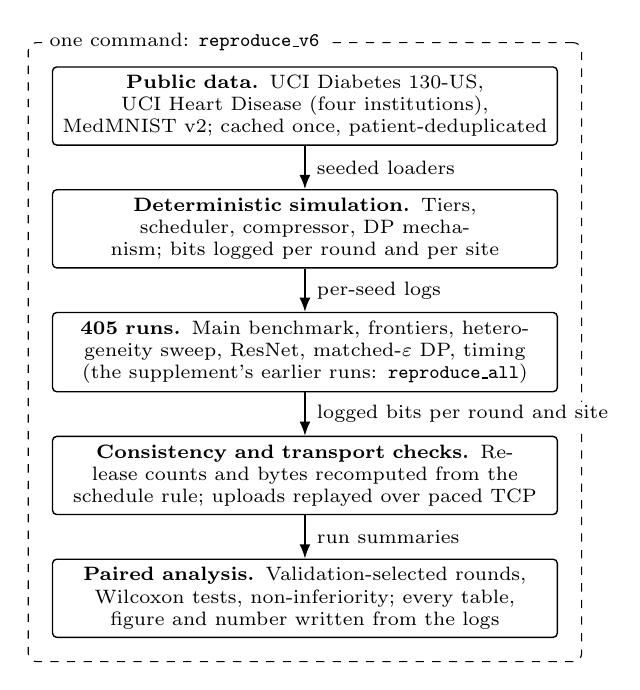
\begin{tikzpicture}[node distance=5.5mm, every node/.style={font=\scriptsize}]
\node[proc, text width=62mm] (d) {\textbf{Public data.} UCI Diabetes 130-US, UCI Heart Disease (four institutions), \mbox{MedMNIST v2}; cached once, patient-deduplicated};
\node[proc, text width=62mm, below=of d] (s) {\textbf{Deterministic simulation.} Tiers, scheduler, compressor, DP mechanism; bits logged per round and per site};
\node[proc, text width=62mm, below=of s] (r) {\textbf{\num{auRunsVsix} runs.} Main benchmark, frontiers, heterogeneity sweep, ResNet, matched-$\varepsilon$ DP, timing (the supplement's earlier runs: \texttt{reproduce\_all})};
\node[proc, text width=62mm, below=of r] (e) {\textbf{Consistency and transport checks.} Release counts and bytes recomputed from the schedule rule; uploads replayed over paced TCP};
\node[proc, text width=62mm, below=of e] (a) {\textbf{Paired analysis.} Validation-selected rounds, Wilcoxon tests, non-inferiority; every table, figure and number written from the logs};
\draw[arr] (d) -- node[lab, right=1mm] {seeded loaders} (s);
\draw[arr] (s) -- node[lab, right=1mm] {per-seed logs} (r);
\draw[arr] (r) -- node[lab, right=1mm] {logged bits per round and site} (e);
\draw[arr] (e) -- node[lab, right=1mm] {run summaries} (a);
\begin{scope}[on background layer]
\node[grp, fit=(d)(s)(r)(e)(a), inner sep=3mm, label={[font=\scriptsize, fill=white, inner sep=2pt, anchor=west, xshift=2mm]north west:one command: \texttt{reproduce\_v6}}] {};
\end{scope}
\end{tikzpicture}
\caption{Study pipeline from the public data to every reported number. All stages run from one command, and the determinism check runs first.}
\label{fig:pipeline}
\end{figure}

\textbf{Metrics.} Each site's patients are split into training, validation and test sets (70/10/20\%, patient-grouped), and every method is evaluated on each site's test split with that site's own parameters, sample-weighted; single-class splits are excluded identically for every method. The primary metric is the test AUROC at the round with the highest validation AUROC (the earliest on ties), with the bytes uploaded up to that round; test data never select anything. Secondary metrics are the mean over the last ten rounds, the mean over the post-synchronisation rounds of the last twenty, and the final round. Calibration is reported as ECE and Brier score~\cite{vancalster2019}, before and after Platt scaling~\cite{platt1999} on each site's validation split, and per-site results as the worst-site AUROC. Fig.~\ref{fig:pipeline} summarises the study.

\textbf{Problem statement.} Given a quota $\rho$ on the payload fraction (\ref{eq:payload}), optionally a cap $\pi$ on the payload of any one round and a budget $(\varepsilon,\delta)$, choose the intervals $\mathbf K$ and phases such that the validation-selected personalised AUROC is non-inferior to full-rate personalisation and is at least that of the best uniform period at the same bytes. Under DP the schedule must be fixed before training, because the accountant charges only data-independent releases. Per-site non-inferiority is reported descriptively, not tested.

\section{Quota-Constrained Multi-Rate Scheduling}
\label{sec:method}

The scheduler separates \emph{what} is sent (tiers), \emph{when} (per-tier intervals chosen under the quota), \emph{how large} (an optional compressor) and \emph{how private} (the DP mechanism and its accountant). Fig.~\ref{fig:arch} shows the architecture. The server-side controller observes the received slices, the sites observe only the broadcast, and the link and the privacy mechanism sit between them.

\begin{figure*}[t]
\centering
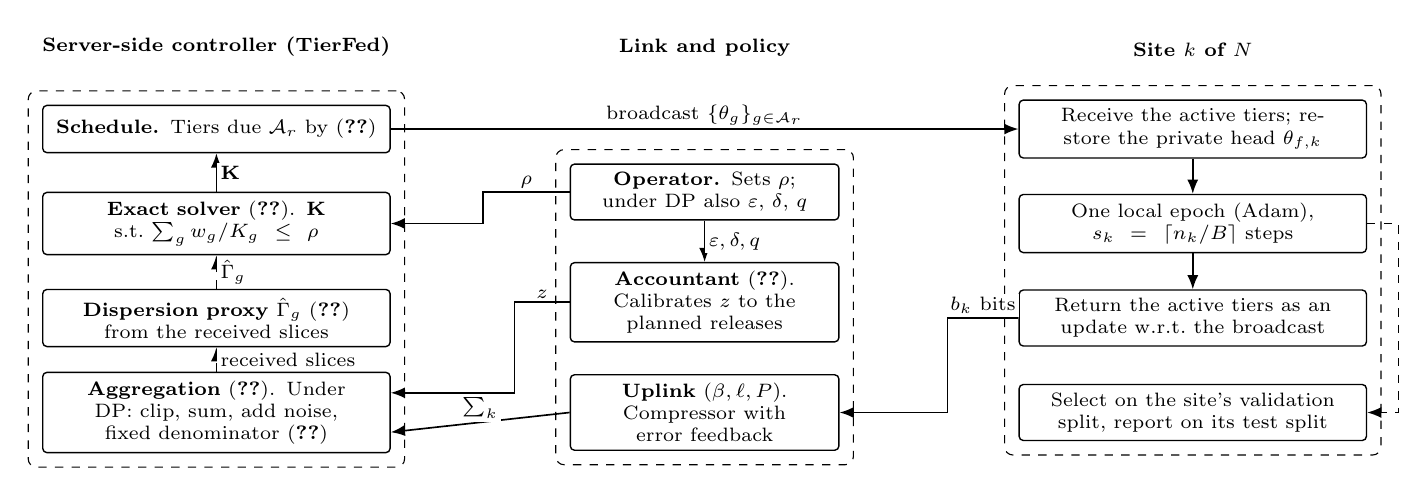
\begin{tikzpicture}[x=1mm,y=1mm]
\node[hdr] at (0,8) {Server-side controller (\tierfed{})};
\node[hdr] at (62,8) {Link and policy};
\node[hdr] at (124,8) {Site $k$ of $N$};
% server column
\node[srvbox, text width=42mm] (sched) at (0,0)   {\textbf{Schedule.} Tiers due $\mathcal A_r$ by (\ref{eq:due})};
\node[srvbox, text width=42mm] (solve) at (0,-12) {\textbf{Exact solver} (\ref{eq:ip}). $\mathbf K$ s.t.\ $\sum_g w_g/K_g\le\rho$};
\node[srvbox, text width=42mm] (disp)  at (0,-24) {\textbf{Dispersion proxy} $\Gh_g$ (\ref{eq:gammahat}) from the received slices};
\node[srvbox, text width=42mm] (agg)   at (0,-36) {\textbf{Aggregation} (\ref{eq:agg}). Under DP: clip, sum, add noise, fixed denominator (\ref{eq:dp})};
% link column
\node[lnkbox, text width=32mm] (op)   at (62,-8)  {\textbf{Operator.} Sets $\rho$; under DP also $\varepsilon$, $\delta$, $q$};
\node[lnkbox, text width=32mm] (acc)  at (62,-22) {\textbf{Accountant} (\ref{eq:rdp}). Calibrates $z$ to the planned releases};
\node[lnkbox, text width=32mm] (link) at (62,-36) {\textbf{Uplink} $(\beta,\ell,P)$. Compressor with error feedback};
% site column
\node[stebox, text width=42mm] (bcast) at (124,0)   {Receive the active tiers; restore the private head $\theta_{f,k}$};
\node[stebox, text width=42mm] (train) at (124,-12) {One local epoch (Adam), $s_k=\lceil n_k/B\rceil$ steps};
\node[stebox, text width=42mm] (ret)   at (124,-24) {Return the active tiers as an update w.r.t.\ the broadcast};
\node[stebox, text width=42mm] (eval)  at (124,-36) {Select on the site's validation split, report on its test split};
\begin{scope}[on background layer]
\node[grp, fit=(sched)(solve)(disp)(agg)] {};
\node[grp, fit=(op)(acc)(link)] {};
\node[grp, fit=(bcast)(train)(ret)(eval)] {};
\end{scope}
% data path down the round (solid)
\draw[arr] (sched.east) -- node[lab, above] {broadcast $\{\theta_g\}_{g\in\mathcal A_r}$} (bcast.west);
\draw[arr] (bcast.south) -- (train.north);
\draw[arr] (train.south) -- (ret.north);
\draw[arr] (ret.west) -- ++(-9,0) node[lab, above, pos=0.5] {$b_k$ bits} |- (link.east);
\draw[arr] (link.west) -- node[lab, above] {$\sum_k$} ([yshift=-2.5mm]agg.east);
% policy inputs (solid)
\draw[arr] (op.west) -- ++(-11,0) node[lab, above, pos=0.5] {$\rho$} |- (solve.east);
\draw[arr] (op.south) -- node[lab, right] {$\varepsilon,\delta,q$} (acc.north);
\draw[arr] (acc.west) -- ++(-7,0) node[lab, above, pos=0.5] {$z$} |- ([yshift=2.5mm]agg.east);
% measurements fed back (dashed)
\draw[meas] (agg.north) -- node[lab, right] {received slices} (disp.south);
\draw[meas] (disp.north) -- node[lab, right] {$\Gh_g$} (solve.south);
\draw[arr]  (solve.north) -- node[lab, right] {$\mathbf K$} (sched.south);
\draw[meas] (train.east) -- ++(4,0) |- (eval.east);
\end{tikzpicture}
\caption{Scheduler and environment. Solid arrows carry data and policy inputs; dashed arrows are measurements fed back. Under DP the dashed path from the received slices to the solver is cut and the schedule is planned before training (Section~\ref{sec:method-privacy}).}
\label{fig:arch}
\end{figure*}

\subsection{Dispersion Measurement}
\tierfed{} estimates the heterogeneity of each tier from the dispersion of the slices it receives. For tier $g$ with tensors $j\in g$,
\begin{equation}
\Gh_g^{(r)}=\frac{\sum_{j\in g}\frac1{|\mathcal S_r|}\sum_{k\in\mathcal S_r}\big\|\theta_{k,j}^{(r)}-\bar\theta_j^{(r)}\big\|_2^2}{\sum_{j\in g}\big\|\bar\theta_j^{(r)}\big\|_2^2+\xi_0},
\label{eq:gammahat}
\end{equation}
a scale-free ratio ($\xi_0=10^{-12}$) that makes tiers of different magnitude comparable. It exists only for tiers received in round $r$; otherwise the last value is carried forward. The received slices result from $m_g=(r-t_g)\,s$ local steps since the tier's last synchronisation $t_g$, and the standard drift lemma of local SGD~\cite{stich2019,khaled2020} bounds the expected numerator by a term of order $\eta^2(m_g\sigma_g^2+m_g^2\Gamma_g)$. $\Gh_g$ can therefore grow quadratically with the interval that produced it, so the controller partly measures its own decisions. The debiased proxy $\tilde\Gamma_g=\Gh_g/(r-t_g)^2$ removes the quadratic growth of the heterogeneity term; it is released as an option but not evaluated here.

\subsection{The Programme and Its Closed Form}
\emph{Bound.} The analysis concerns the shared backbone with the private heads frozen; the personalisation gap this introduces is measured empirically. Assume block-separable $L$-smoothness (the gradient of tier $g$ is $L$-Lipschitz in $\theta_g$ and does not depend on the other tiers; this ignores cross-tier coupling and is the main idealisation), unbiased stochastic gradients with per-tier variance $\sigma_g^2$, bounded per-tier heterogeneity $\frac1N\sum_k\|\nabla_gF_k(\theta)-\nabla_gF(\theta)\|^2\le\Gamma_g$, $F\ge F^\star$~\cite{stich2019,wang2021coop}, and the same number $s$ of local steps at every site. With unequal $s_k$, plain averaging converges towards a reweighted objective~\cite{wang2020fednova}; the experiments keep $s_k=\lceil n_k/B\rceil$ and do not normalise.
\begin{proposition}[Multi-rate local-SGD bound]
\label{prop:bound}
With local SGD of step size $\eta$ and tier $g$ averaged every $K_g$ rounds, there are absolute constants $c_0,c_1,c_2$ such that for $\eta\le c_0/(LK_{\max}s)$,
\begin{align}
\frac1R\sum_{r=1}^R\mathbb E\big\|\nabla F(\bar\theta_r)\big\|^2
&\le \frac{c_1(F(\bar\theta_1)-F^\star)}{\eta sR}+c_1\eta L\sum_g\frac{\sigma_g^2}{N}\notag\\
&\quad+c_2\,\eta^2L^2s^2\sum_g K_g^2\big(\Gamma_g+\sigma_g^2\big).
\label{eq:bound}
\end{align}
\end{proposition}
The proof applies the perturbed-iterate argument of~\cite{wang2021coop} blockwise (supplement, Section~S2). In the bound, a long interval is cheap only for a tier with small $\Gamma_g+\sigma_g^2$.

\emph{Programme.} Given a quota $\rho$ the controller solves
\begin{equation}
\mathbf K^\star=\arg\min_{K_g\in\{1,\dots,K_{\max}\}}\sum_{g\in\mathcal G_{\mathrm{sh}}}K_g^2\,\Gh_g\ \ \text{s.t.}\ \sum_{g\in\mathcal G_{\mathrm{sh}}}\frac{w_g}{K_g}\le\rho .
\label{eq:ip}
\end{equation}
It keeps the $K_g^2\Gamma_g$ term of (\ref{eq:bound}). The $K_g^2\sigma_g^2$ term is not separately estimable from parameter dispersion, which mixes it with the heterogeneity term, and the common factor $s^2$ does not change the minimiser. With the head private, $\mathcal G_{\mathrm{sh}}=\{\mathrm s,\mathrm m\}$ and $K_{\max}=8$, so the programme has 64 candidates and is solved by enumeration, with ties broken towards the denser schedule.

\begin{proposition}[Closed form and the value of differentiation]
\label{prop:cuberoot}
Let $\Gamma_g>0$, $w_g>0$, $\sum_gw_g=1$, and relax $K_g$ to the positive reals. Then (\ref{eq:ip}) has the unique minimiser
\begin{equation}
K_g^\star=\Big(\frac{w_g}{\Gamma_g}\Big)^{1/3}\frac{S}{\rho},\qquad S=\sum_hw_h^{2/3}\Gamma_h^{1/3},
\label{eq:cuberoot}
\end{equation}
with value $J^\star=S^3/\rho^2$. The uniform interval $K=1/\rho$ costs $J_{\mathrm u}=\sum_g\Gamma_g/\rho^2$, and
\begin{equation}
\Psi=1-\frac{J^\star}{J_{\mathrm u}}=1-\frac{S^3}{\sum_g\Gamma_g}\in[0,1),
\label{eq:psi}
\end{equation}
with $\Psi=0$ if and only if $w_g/\Gamma_g$ is equal for all tiers. When $1/\rho$ is an integer, no integer schedule lowers the objective of (\ref{eq:ip}) below that of the uniform period by more than the fraction $\Psi$.
\end{proposition}
The objective is strictly convex and increasing in every $K_g$ and the feasible set is convex, so the quota binds and the KKT point is the minimiser; $S^3\le(\sum_gw_g)^2\sum_g\Gamma_g$ is H\"older's inequality with exponents $3/2$ and $3$; the integer statement holds because the relaxation bounds the integer optimum from below and $K=1/\rho$ is integer-feasible (supplement, Section~S2). Two consequences shape the evaluation. The interval ratio $K_a/K_b=(w_a\Gamma_b/w_b\Gamma_a)^{1/3}$ compresses differences: a factor of eight in payload-to-dispersion ratio is needed for a factor of two in interval, so tiers with similar ratios collapse onto one interval after rounding. And $\Psi$ is scale-free in $\Gamma$, so the common bias of $\Gh_g$ cancels when it is measured at the end of warm-up, where every tier has been synchronised every round; it then predicts, before any sparse round, how much a per-tier schedule can gain over a uniform one.

\subsection{Schedule Rule, Phases and the Quota}
Rounds are indexed $r=1,\dots,R$. The first $T_w$ rounds synchronise every shared tier, and thereafter tier $g$ is due when
\begin{equation}
\mathcal A_r=\begin{cases}\mathcal G_{\mathrm{sh}}, & r\le T_w,\\ \{g:\ (r-T_w-\phi_g)\bmod K_g=0\}, & r>T_w,\end{cases}
\label{eq:due}
\end{equation}
with phase $\phi_g=0$ unless staggered. The fixed periods, the DP planner and the accountant all use this one rule, and the consistency check of Section~\ref{sec:results-check} recomputes every release from it. Adaptive \tierfed{} sends tier $g$ when $r-t_g\ge K_g$, which coincides with (\ref{eq:due}) whenever $\mathbf K$ is constant after warm-up. $T_w=5$ and $K_{\max}=8$ are fixed across every dataset, architecture, loss and privacy setting. Fig.~\ref{fig:round} shows one server round.

\emph{Phases and the peak.} A mean quota does not bound the payload $P_r$ of a single round: aligned tiers coincide and send the full shared payload. Two tiers with phases $\phi_a,\phi_b$ are never due in the same round if and only if $\phi_a-\phi_b\not\equiv0\pmod{\gcd(K_a,K_b)}$ (Chinese remainder theorem), so with $\gcd\ge2$ the offset $\lfloor\gcd/2\rfloor$ separates them and bounds the post-warm-up peak by $\max_gw_g$ at an unchanged mean; with co-prime intervals no phase helps. The staggered variant adds $\max_{r>T_w}P_r\le\pi$ to (\ref{eq:ip}) and checks it over one hyper-period $\mathrm{lcm}(\mathbf K)$. A full-rate warm-up still sends the whole payload, so the warm-up rounds can be sent at eight bits.

\emph{The quota.} Solving (\ref{eq:ip}) with $\rho$ bounds $\Pi_\infty$ of (\ref{eq:payload}), not the realised $\Pi_R$: a warm-up of $T_w$ rounds at payload fraction $c_w$ adds $T_w(c_w-\Pi_\infty)/R$ to the realised fraction. A quota over all rounds is met by solving with $\rho'=(\rho R-c_wT_w)/(R-T_w)$; both forms are reported, and the realised $\Pi_R$ is read from the logs.

\begin{figure}[t]
\centering
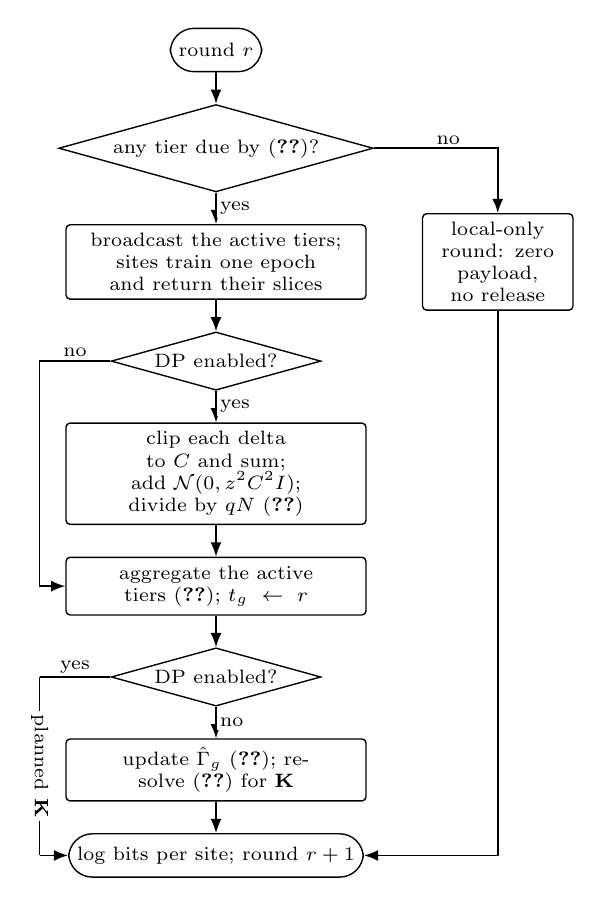
\begin{tikzpicture}[node distance=4mm and 6mm, every node/.style={font=\scriptsize}]
\node[term] (start) {round $r$};
\node[dec, below=of start] (due) {any tier due by (\ref{eq:due})?};
\node[proc, text width=36mm, below=of due] (bc) {broadcast the active tiers; sites train one epoch and return their slices};
\node[dec, below=of bc] (dp) {DP enabled?};
\node[proc, text width=36mm, below=of dp] (priv) {clip each delta to $C$ and sum;\\ add $\mathcal N(0,z^2C^2I)$;\\ divide by $qN$ (\ref{eq:dp})};
\node[proc, text width=36mm, below=of priv] (ag) {aggregate the active tiers (\ref{eq:agg}); $t_g\leftarrow r$};
\node[dec, below=of ag] (dp2) {DP enabled?};
\node[proc, text width=36mm, below=of dp2] (upd) {update $\Gh_g$ (\ref{eq:gammahat}); re-solve (\ref{eq:ip}) for $\mathbf K$};
\node[term, below=of upd] (next) {log bits per site; round $r+1$};
\node[proc, text width=17mm, right=7mm of bc] (local) {local-only round: zero payload, no release};
\draw[arr] (start) -- (due);
\draw[arr] (due) -- node[lab, right] {yes} (bc);
\draw[arr] (due.east) -| node[lab, above, pos=0.3] {no} (local);
\draw[arr] (local.south) |- (next.east);
\draw[arr] (bc) -- (dp);
\draw[arr] (dp) -- node[lab, right] {yes} (priv);
\draw[arr] (dp.west) -- ++(-9mm,0) node[lab, above, pos=0.5] {no} |- (ag.west);
\draw[arr] (priv) -- (ag);
\draw[arr] (ag) -- (dp2);
\draw[arr] (dp2) -- node[lab, right] {no} (upd);
\coordinate (k1) at ($(dp2.west)+(-9mm,0)$);
\coordinate (k2) at (k1 |- next.west);
\draw[line width=0.6pt] (dp2.west) -- node[lab, above] {yes} (k1);
\draw[line width=0.6pt] (k1) -- node[lab, sloped, midway] {planned $\mathbf K$} (k2);
\draw[arr] (k2) -- (next.west);
\draw[arr] (upd) -- (next);
\end{tikzpicture}
\caption{One server round. Under DP the schedule is fixed before training and the dispersion feedback is never computed from the private slices.}
\label{fig:round}
\end{figure}

\emph{Compression.} A compressor that emits a fraction $\kappa\in(0,1]$ of the float32 bits multiplies the upload, $B=R\,|\mathcal S|\,\Pi_R(\mathbf K)\,\kappa\,32\,d_{\mathrm{sh}}$ bits for $d_{\mathrm{sh}}$ shared parameters; it acts on each site's update relative to the broadcast, with error feedback, and the bits it emits are counted.

\subsection{Privacy: Threat Model, Mechanism and Eligible Schedules}
\label{sec:method-privacy}
\emph{Threat model.} Sites send their updates over TLS to an aggregator that is trusted to apply the mechanism and sees raw updates, as in central DP-FedAvg~\cite{mcmahan2018dp}. Consumers of the released models, the other sites among them, see every broadcast, and central DP protects the released aggregates against them. A passive network observer cannot read the payloads but sees when each site transmits and how many bytes, which is exactly the schedule; a schedule that depends on client data therefore leaks even when every payload is encrypted. Secure aggregation with distributed noise~\cite{kairouz2021ddg} would remove the trust in the aggregator but not this metadata, and poisoning is out of scope.

\emph{Mechanism.} Each round every site joins the cohort $\mathcal S_r$ independently with probability $q$; $q=1$, full participation, is the primary cross-silo setting and $q<1$ a sensitivity analysis. The server clips every participating site's returned delta and adds noise to the sum before dividing by the \emph{fixed} expected cohort size,
\begin{equation}
\tilde\Delta=\frac1{qN}\Big(\sum_{k\in\mathcal S_r}\Delta_k\min\big(1,\tfrac{C}{\|\Delta_k\|_2}\big)+\mathcal N(0,z^2C^2I)\Big),
\label{eq:dp}
\end{equation}
the fixed-denominator DP-FedAvg estimator~\cite{mcmahan2018dp}, so that adding or removing one site changes the sum by at most $C$ in $\ell_2$ and the denominator reveals nothing about the realised cohort; a planned release whose cohort is empty still adds noise. The mechanism is applied by the server to every method identically.

\emph{Accountant.} Over the $R_{\mathrm{tx}}$ planned releases the R\'enyi DP of the Poisson-subsampled Gaussian mechanism is composed at integer orders~\cite{mironov2019sgm},
\begin{align}
\varepsilon_\alpha&=\frac{R_{\mathrm{tx}}}{\alpha-1}\log\sum_{k=0}^{\alpha}\binom{\alpha}{k}(1-q)^{\alpha-k}q^ke^{\frac{k^2-k}{2z^2}},\notag\\
\varepsilon&=\min_\alpha\Big\{\varepsilon_\alpha+\frac{\log(1/\delta)}{\alpha-1}\Big\},
\label{eq:rdp}
\end{align}
with $\delta=10^{-5}$; for $q=1$ this reduces to $R_{\mathrm{tx}}\alpha/(2z^2)$~\cite{mironov2017}. The implementation reproduces the TensorFlow-Privacy MNIST reference ($\varepsilon\approx3.0$) and the $q=1$ closed form as unit tests. At $q=1$ the exact privacy of $R_{\mathrm{tx}}$ Gaussian releases is $\mu$-Gaussian DP with $\mu=\sqrt{R_{\mathrm{tx}}}/z$~\cite{dong2022gdp,balle2018}. Both accountants depend on $R_{\mathrm{tx}}$ only through $R_{\mathrm{tx}}/z^2$, so the exact one lowers every method's noise multiplier by the same factor, \num{gdpSigmaCutEightPct}--\num{gdpSigmaCutOnePct}\% for $\varepsilon^\star$ from 8 to 1. The comparison at matched $\varepsilon$ is therefore unchanged, and every reported $\varepsilon$ is an upper bound; $z$ is calibrated to each method's own release count by bisection on (\ref{eq:rdp}).

\emph{Which schedules are covered.} The accountant covers a release only if the decision to release does not depend on the private data. This holds for FedAvg, FedProx, FedPer, local training, a fixed period and the planner below, whose release rounds are fixed before training, and not for adaptive \tierfed{}, AdaComm, LAG or FedLAMA, whose schedules are functions of client updates or losses; the released code refuses to run them under DP. Data-dependent release decisions are a known pattern, which privacy filters and odometers~\cite{rogers2016odometer} and the sparse vector technique~\cite{lyu2017svt} charge for; the point here is that FL schedulers take such decisions without charging for them. DP-FTRL~\cite{kairouz2021ftrl} and matrix-factorisation mechanisms~\cite{choquette2023banded} suit full participation but also need data-independent release rounds; they are not evaluated.

\emph{Planning under a privacy budget (\tierfed{}-DP).} A planner that respects the accountant chooses $\mathbf K$ before training from public quantities only, $(\varepsilon^\star,\delta)$, $q$, $R$, $T_w$, $w_g$ and $\rho$. For each candidate it computes the release set of (\ref{eq:due}), the smallest $z(\mathbf K)$ that keeps those releases $(\varepsilon^\star,\delta)$-DP, and minimises
\begin{equation}
J(\mathbf K)=\frac{\sum_g w_gK_g^2}{K_{\max}^2}+\lambda\,\frac{\sum_{r}P_r(\mathbf K)\,z(\mathbf K)^2}{\sum_{r}P_r(\mathbf 1)\,z(\mathbf 1)^2},
\label{eq:jdp}
\end{equation}
the drift term of (\ref{eq:bound}) under a flat heterogeneity prior plus the injected noise energy, each normalised by its worst case, with $\lambda=1$. Fewer releases need less noise per release but drift more. Under the flat prior, $\Gamma_g\propto w_g$ and Proposition~\ref{prop:cuberoot} gives $\Psi=0$, so the planner can only choose equal intervals; it is evaluated as an ablation, not claimed as a contribution.

\section{Experimental Setup}
\label{sec:setup}
Every method is run under the protocol of Section~\ref{sec:system} on the same seeds and splits, and every number is read from the logs. This section lists the experiment families, the baselines and bounds, the privacy and timing experiments, and the statistics that decide each comparison.

\begin{table}[t]
\caption{Experiment families of the v6 runs, counted from the logs: data and sites, configurations, seeds and runs}
\label{tab:families}
\centering\footnotesize
\fit{\gen{au_families}}
\end{table}

\textbf{Experiment families.} Table~\ref{tab:families} lists the \num{auRunsVsix} runs: the main comparison; the iso-byte frontier, each method with its own knob swept; the label-skew sweep and the ResNet backbone, which test the regimes to which Proposition~\ref{prop:cuberoot} points; matched-$\varepsilon$ DP and the timing side channel for the privacy claims; and the peak-aware variants. Results of the earlier final-round protocol (compression, real institutions, imaging, scaling, a wide model) are in the supplement.

\textbf{Baselines and bounds.} \emph{Full rate:} FedAvg~\cite{mcmahan2017}, FedProx~\cite{li2020fedprox} and FedPer~\cite{arivazhagan2019}, the reference for the non-inferiority tests. \emph{Round-sparse:} AdaComm~\cite{wang2019adacomm}, LAG~\cite{chen2018lag} with sample weighting and, for comparison with earlier versions, with the equal weights used there, a FedLAMA-style per-layer interval rule reimplemented from its published description~\cite{lee2023fedlama}, and fixed periods on (\ref{eq:due}) with the same private head and warm-up as \tierfed{}. \emph{Bounds:} local training without communication, a centralised MLP trained on the pooled training splits of all sites for the same number of passes, and gradient boosting~\cite{ke2017lightgbm}; all three are scored on the same per-site test splits with the round, epoch or iteration chosen on validation. SCAFFOLD, whose control variates fit Adam poorly, is reported with SGD in the supplement.

\textbf{Differential privacy.} FedPer, fixed periods $K=4$ and $K=8$, one-shot federation (no warm-up, one release in round $R$, after a data-independent broadcast of the initial model) and the planner run at $\varepsilon^\star=4$, $\delta=10^{-5}$, $q=1$, $C=1$, each with $z$ calibrated to its own release count. Local training is the $\varepsilon=0$ reference on the same splits. The $q<1$ sweeps over $\varepsilon^\star\in\{1,2,4,8\}$ on 20 and 100 sites are in the supplement.

\textbf{Timing side channel.} One target site holds half of its labels flipped (shifted world) or none (clean world). A passive observer sees which rounds carry traffic and how many bytes each site sends, and reduces each run to an observable $o$: the rounds with traffic, the target's rounds, the target's bytes or the bytes of all sites. Its power is the Mann--Whitney AUC over the $n_1$ shifted and $n_0$ clean runs,
\begin{equation}
\mathrm{AUC}=\frac1{n_1n_0}\sum_{i=1}^{n_1}\sum_{j=1}^{n_0}\Big(\mathbb 1\big[o^{(1)}_i>o^{(0)}_j\big]+\tfrac12\,\mathbb 1\big[o^{(1)}_i=o^{(0)}_j\big]\Big),
\label{eq:auc}
\end{equation}
where 0.5 means that the schedule reveals nothing; an AUC of at least 0.75 on any observable is reported as a leak.

\textbf{Statistics.} All comparisons are paired across seeds. Two primary contrasts were fixed in the code before the runs, with the metric and both thresholds: \tierfed{} against FedPer, and \tierfed{} against the best uniform period at matched bytes. With $\mathcal U$ the uniform periods run in a setting, $B$ the mean upload and $\bar A^{\mathcal V}$ the mean validation AUROC at $\hat r$, that period and the gain over it are
\begin{equation}
\begin{gathered}
K_{\mathrm u}=\arg\max_{K\in\mathcal U:\,B_K\le1.05\,B_{\mathrm{TF}}}\bar A^{\mathcal V}_K,\\
\Delta_{\mathrm u}=\frac1S\sum_{s=1}^{S}\big(A^{\mathcal T}_{\mathrm{TF},s}-A^{\mathcal T}_{K_{\mathrm u},s}\big),
\end{gathered}
\label{eq:gate}
\end{equation}
over the $S$ seeds both share; every other comparison is exploratory. Tests are two-sided Wilcoxon signed-rank tests and intervals are percentile bootstrap intervals over seeds. The gate first required a Holm-corrected $p<0.05$, which 5 or 6 seeds cannot reach, so $\Delta_{\mathrm u}$ is read from its interval: a setting counts as a gain only when the 95\% interval excludes zero and $\Delta_{\mathrm u}\ge0.005$ AUROC\ifflag{auRouteA}{}{; no setting passes either rule}. A difference below 0.005 is not called relevant, whatever its $p$. Non-inferiority to FedPer is tested one-sided,
\begin{equation}
H_0:\ \mathbb E[d]\le-\Delta_{\mathrm{NI}},\qquad d=A^{\mathcal T}_{\text{method}}(\hat r)-A^{\mathcal T}_{\text{FedPer}}(\hat r),
\label{eq:ni}
\end{equation}
by the signed-rank test on $d+\Delta_{\mathrm{NI}}$ at $\Delta_{\mathrm{NI}}=0.01$ and, as a sensitivity margin, 0.005. Repeated runs are bit-identical on one machine. On a second machine every data-independent schedule \ifflag{xmachineBytesIdentical}{sends the same bytes}{changes its bytes}, but the AUROC of a single run can move by up to \num{xmachineAurocDiff} (Section~\ref{sec:results-check}), so every comparison is computed within one machine.

\section{Results}
\label{sec:results}

Every table body and every number in this section is generated from the per-seed logs by the released analysis script. Unless stated otherwise, values are means over ten seeds on Diabetes 130-US with the MLP backbone; $p$-values are from paired tests across seeds.

\subsection{Main benchmark}
\label{sec:results-fixed}

\begin{table*}[t]
\caption{Main benchmark (Diabetes 130-US, 20 sites, 60 rounds, 10 seeds). Final-round federated AUROC (mean $\pm$ SD), AUPRC, early-stopped AUROC, pooled AUROC, cumulative upload per site, number of transmitting rounds, and one-sided non-inferiority $p$-values against FedPer at $\delta_{\mathrm{NI}}=0.01$ on AUROC and AUPRC.}
\label{tab:main}
\centering\small
\begin{tabular}{lrcccccccc}
\toprule
Method & $n$ & AUROC & AUPRC & ES-AUROC & Pooled & Upload (MB) & Tx rounds & NI$_{\mathrm{AUROC}}$ $p$ & NI$_{\mathrm{AUPRC}}$ $p$\\
\midrule
\gen{main_diabetes_mlp}
\bottomrule
\end{tabular}
\end{table*}

\begin{table}[t]
\caption{Holm-corrected paired comparisons on final AUROC against FedPer (10 seeds): mean difference, BCa 95\% interval, corrected $p$, paired $d_z$.}
\label{tab:holm}
\centering\small
\begin{tabular}{lcccc c}
\toprule
Comparison & $\Delta$ & 95\% CI & $p_{\mathrm{Holm}}$ & $d_z$ & Sig.\\
\midrule
\gen{holm_diabetes_mlp}
\bottomrule
\end{tabular}
\end{table}

Table~\ref{tab:main} reports the main benchmark. Full-rate FedPer reaches \num{diabetesmlpFedperAuroc}~AUROC at \num{diabetesmlpFedperUploadMb}~MB per site. \tierfed{} at $\rho=0.25$ reaches \num{diabetesmlpTierfedAuroc} (paired difference \num{mainTfVsFedperDiff}, $p=\num{mainTfVsFedperP}$) at \num{diabetesmlpTierfedUploadMb}~MB, transmitting in \num{factorialTierfedTxRounds} of 60 rounds; it is \ifflag{diabetesmlpTierfedNonInferiorAuroc}{non-inferior to FedPer on AUROC ($p=\num{diabetesmlpTierfedNiAurocP}$)}{not non-inferior to FedPer on AUROC ($p=\num{diabetesmlpTierfedNiAurocP}$)} and \ifflag{diabetesmlpTierfedNonInferiorAuprc}{on AUPRC ($p=\num{diabetesmlpTierfedNiAuprcP}$)}{not on AUPRC ($p=\num{diabetesmlpTierfedNiAuprcP}$)}. The round-sparse baselines are at least as accurate: AdaComm reaches \num{diabetesmlpAdacommAuroc} at \num{diabetesmlpAdacommUploadMb}~MB (\tierfed{} minus AdaComm: \num{mainTfVsAdacommDiff}, $p=\num{mainTfVsAdacommP}$), and the fixed multi-rate schedule ($K_{\mathrm s}=5$, $K_{\mathrm m}=2$) reaches \num{diabetesmlpFixedAuroc} at \num{diabetesmlpFixedUploadMb}~MB. LAG at its default threshold never skips an upload and is equivalent to full-rate averaging (\num{diabetesmlpLagAuroc}); SCAFFOLD with the Adam local solver used for every method underperforms (\num{diabetesmlpScaffoldAuroc}) and is reported with its native SGD solver in Table~\ref{tab:baselines}. Early-stopped AUROC is within a narrow band for all methods, so no conclusion depends on the final round.

\textbf{Synchronising less does not hurt here.} Table~\ref{tab:periods} sweeps the fixed schedule's periods. A uniform period of four rounds for both shared tiers reaches \num{periodsKsFourKmFourAuroc} at \num{periodsKsFourKmFourUploadMb}~MB, the best accuracy of any configuration in this study; only a long slow-tier period ($K_{\mathrm s}=8$) costs accuracy (\num{periodsKsEightKmOneAuroc} with $K_{\mathrm m}=1$). Table~\ref{tab:factorial} separates the private head from the schedule: FedPer and FedAvg are level (\num{factorialFedperAuroc} and \num{factorialFedavgAuroc}), so the head does not matter on this data, and \tierfed{} with and without the head is also level (\num{factorialTierfedAuroc} and \num{factorialTierfedNoheadAuroc}). The modest gain of every sparse schedule over full-rate averaging is consistent with additional local training acting as personalisation. An earlier version of this work reported that fixed multi-rate schedules lose about 0.05~AUROC to FedPer; that finding was produced by encounters of the same patient appearing in training and test splits, and by a fallback rule that sent the medium tier whenever no tier was due. Both are corrected here and the finding does not reproduce.

\begin{table}[t]
\caption{Fixed-schedule period sweep $(K_{\mathrm s},K_{\mathrm m})$, 10 seeds; rounds with no tier due are local-only.}
\label{tab:periods}
\centering\small
\begin{tabular}{lrcc}
\toprule
$(K_{\mathrm s},K_{\mathrm m})$ & $n$ & AUROC & Upload (MB)\\
\midrule
\gen{periods}
\bottomrule
\end{tabular}
\end{table}

\begin{table}[t]
\caption{Attribution (10 seeds): private head $\times$ schedule, and \tierfed{} with and without the private head.}
\label{tab:factorial}
\centering\small
\begin{tabular}{lrccc}
\toprule
Cell & $n$ & AUROC & AUPRC & Upload (MB)\\
\midrule
\gen{factorial}
\bottomrule
\end{tabular}
\end{table}

\subsection{The budget knob and the controller}
\label{sec:results-budget}

\begin{table}[t]
\caption{Quota sweep for \tierfed{} (10 seeds): accuracy, upload, realised payload fraction, mean intervals chosen by the exact solver, and the share of post-warm-up rounds in which the two shared tiers received different intervals.}
\label{tab:budget}
\centering\small
\resizebox{\columnwidth}{!}{%
\begin{tabular}{lrcccccc c}
\toprule
$\rho$ & $n$ & AUROC & AUPRC & Upload (MB) & Realised & $\bar K_{\mathrm s}$ & $\bar K_{\mathrm m}$ & Differentiated (\%)\\
\midrule
\gen{budget}
\bottomrule
\end{tabular}}
\end{table}

\begin{table}[t]
\caption{Exact solver versus greedy doubling at two quotas (10 seeds).}
\label{tab:solver}
\centering\small
\begin{tabular}{lrcc}
\toprule
$\rho$ / solver & $n$ & AUROC & Upload (MB)\\
\midrule
\gen{solver}
\bottomrule
\end{tabular}
\end{table}

Table~\ref{tab:budget} shows that $\rho$ behaves as an operator knob: upload rises monotonically with the quota, from \num{budgetRhoFifteenUploadMb}~MB at $\rho=0.15$ to \num{budgetRhoEightyUploadMb}~MB at $\rho=0.8$. Accuracy is flat above $\rho=0.25$ and drops only at $\rho=0.15$ (\num{budgetRhoFifteenAuroc}); the best quota is $\rho=0.4$ (\num{budgetRhoFortyAuroc} at \num{budgetRhoFortyUploadMb}~MB). The last column is the honest test of the divergence-driven mechanism: at $\rho=0.25$ the solver gave the two shared tiers different intervals in \num{budgetRhoTwentyFiveDiffPct}\% of rounds, at $\rho=0.4$ in \num{budgetRhoFortyDiffPct}\%, and at most in \num{budgetRhoFifteenDiffPct}\% at $\rho=0.15$. On this data the controller mostly reduces to a uniform period chosen to meet the quota, which explains why a well-chosen fixed period performs as well. Where the solvers differ, exactness helps: at $\rho=0.4$ the exact solver reaches \num{budgetRhoFortyAuroc} at \num{budgetRhoFortyUploadMb}~MB against \num{budgetRhoFortyGreedyAuroc} at \num{budgetRhoFortyGreedyUploadMb}~MB for the greedy doubling rule (Table~\ref{tab:solver}).

\begin{table}[t]
\caption{Baseline sweeps (10 seeds): AdaComm initial period $\tau_0$, LAG threshold $\xi$, and the SGD local solver for FedAvg, FedPer, SCAFFOLD and \tierfed{}.}
\label{tab:baselines}
\centering\small
\begin{tabular}{lrcccc}
\toprule
Configuration & $n$ & AUROC & AUPRC & Upload (MB) & Tx rounds\\
\midrule
\gen{baselines}
\bottomrule
\end{tabular}
\end{table}

Table~\ref{tab:baselines} gives the baselines a fair frontier. AdaComm with $\tau_0=8$ is the most byte-efficient configuration without DP (\num{baselinesAdacommTauEightAuroc} at \num{baselinesAdacommTauEightUploadMb}~MB); LAG skips uploads only at $\xi=10^4$, where its accuracy collapses (\num{baselinesLagXiOneZeroZeroZeroZeroAuroc}). With an SGD local solver SCAFFOLD recovers (\num{baselinesScaffoldSgdAuroc}), FedAvg and FedPer improve (\num{baselinesFedavgSgdAuroc}, \num{baselinesFedperSgdAuroc}), and \tierfed{} is lower (\num{baselinesTierfedSgdAuroc}); the ordering of methods therefore depends on the local solver, which we state as a limitation.

\begin{figure}[t]
\centering\fig{fig_frontier}{0.95\columnwidth}
\caption{Accuracy--communication frontier on Diabetes (10 seeds): every method, quota and compressor on one pair of axes.}
\label{fig:frontier}
\end{figure}

\subsection{Scheduling and compression compose}
\label{sec:results-comp}

\begin{table}[t]
\caption{Scheduling $\times$ compression (10 seeds). Compressors act on the update with per-client error feedback. \tierfed{} rows use $\rho=0.25$.}
\label{tab:comp}
\centering\small
\begin{tabular}{lrccc}
\toprule
Method / compressor & $n$ & AUROC & AUPRC & Upload (MB)\\
\midrule
\gen{compression}
\bottomrule
\end{tabular}
\end{table}

Table~\ref{tab:comp} confirms (\ref{eq:compose}): reductions from timing and from message size multiply. 8-bit quantisation alone takes FedPer from \num{compFedperNoneUploadMb} to \num{compFedperQuantEightUploadMb}~MB at unchanged accuracy (\num{compFedperQuantEightAuroc}); \tierfed{} with 8-bit quantisation uploads \num{compTierfedQuantEightUploadMb}~MB (\num{compTierfedQuantEightAuroc}); and \tierfed{} with sparse ternary compression uploads \num{compTierfedStcUploadMb}~MB at \num{compTierfedStcAuroc}, against \num{compFedperStcUploadMb}~MB (\num{compFedperStcAuroc}) for FedPer with the same compressor. Count-sketch compression fails for every method (\num{compFedavgSketchAuroc}, \num{compFedperSketchAuroc}, \num{compTierfedSketchAuroc}): at the sketch width used, the unsketched estimate of the update is too noisy for this model, and we report it rather than tune it away.

\subsection{Network-level cost}
\label{sec:results-net}

\begin{table}[t]
\caption{Network cost of the main benchmark under the link profiles of Table~\ref{tab:profiles}: total communication time on cell-edge NR, LEO satellite and the 6G edge-slice target, uplink energy on cell-edge NR, and the fraction of rounds fitting a 60-s window on cell-edge NR. Means over 10 seeds, computed from measured bits by (\ref{eq:netcost}).}
\label{tab:network}
\centering\small
\resizebox{\columnwidth}{!}{%
\begin{tabular}{lrrrrrr}
\toprule
Method & Upload (MB) & $t$ NR-edge (s) & $t$ LEO (s) & $t$ 6G (s) & $E$ NR-edge (J) & Window (\%)\\
\midrule
\gen{network_diabetes_mlp}
\bottomrule
\end{tabular}}
\end{table}

Table~\ref{tab:network} translates measured bits into what an operator sees. On a cell-edge NR uplink the total communication time of the job falls from \num{NetCellEdgeFedper}~s for FedPer to \num{NetCellEdgeTierfed}~s for \tierfed{}. The model is small, so every method fits the 60-s window on every link profile; the absolute times matter less than the proportional reductions, which carry over to larger models with the same schedule.

\subsection{A wide model on emulated links}
\label{sec:results-emu}
\begin{table}[t]
\caption{Wide MLP (\num{wideParams} parameters) on Diabetes (3 seeds): accuracy and upload.}
\label{tab:wide}
\centering\small
\begin{tabular}{lrccrr}
\toprule
Method & $n$ & AUROC & AUPRC & Upload (MB) & Params\\
\midrule
\gen{wide}
\bottomrule
\end{tabular}
\end{table}

\begin{table*}[t]
\caption{Trace-driven socket emulation of the wide-MLP runs: total emulated upload time (real TCP over paced loopback links), the analytic model's prediction from (\ref{eq:netcost}), their relative difference, total compute time of the slowest site, and wall-clock time to reach AUROC 0.60 and 0.62 (``never'' if not reached in 60 rounds). Means over seeds; the cell-edge profile was emulated for one seed.}
\label{tab:emu}
\centering\small
\begin{tabular}{llrrrrrrr}
\toprule
Profile & Method & $n$ & Emulated (s) & Analytic (s) & Diff.\ (\%) & Compute (s) & $t_{0.60}$ (s) & $t_{0.62}$ (s)\\
\midrule
\gen{emulation}
\bottomrule
\end{tabular}
\end{table*}

With \num{wideParams} parameters, a full-rate upload is several megabytes per site and the link dominates the round on every constrained profile (Table~\ref{tab:emu}). The analytic model agrees with real paced TCP to within \num{emuMaxAbsRelErrPct}\% on every run, so the network costs reported in Table~\ref{tab:network} are not an artefact of the formula; the residual is the RTT term, which the analytic model charges in full and the emulator as a one-way delay, plus transport overhead. Over 60 rounds on cell-edge NR, the emulated upload time is \num{emuNrCellEdgeFedperUploadS}~s for FedPer, \num{emuNrCellEdgeTierfedUploadS}~s for \tierfed{}, \num{emuNrCellEdgeFixedUploadS}~s for the fixed period and \num{emuNrCellEdgeAdacommUploadS}~s for AdaComm. Time to a low target (AUROC 0.60) is not reduced by \tierfed{} (\num{emuNrCellEdgeTierfedTtZeropSix}~s against \num{emuNrCellEdgeFedperTtZeropSix}~s), because the target is reached during the full-rate warm-up; the saving is in the remaining rounds. AdaComm never reaches 0.62 within 60 rounds. On accuracy (Table~\ref{tab:wide}) the wide model favours sparse synchronisation more strongly than the small one: the fixed period reaches \num{wideFixedAuroc}, AdaComm \num{wideAdacommAuroc} and \tierfed{} \num{wideTierfedAuroc}, against \num{wideFedperAuroc} for FedPer and \num{wideFedavgAuroc} for FedAvg; with three seeds this is indicative, and the fixed period is again the most accurate.

\subsection{Attack surface and differential privacy}
\label{sec:results-privacy}

\begin{table}[t]
\caption{Matched-privacy comparison (10 seeds, $C=1$, $\delta=10^{-5}$). Every method is run at the same target $\varepsilon^\star$ with Poisson client sampling at rate $q$; its noise multiplier $\sigma$ is calibrated to its own number of planned releases with the subsampled-Gaussian accountant (\ref{eq:rdp}). Achieved $\varepsilon$, final-round AUROC and AUPRC, and upload. Only data-independent schedules are eligible (Section~\ref{sec:security-dp}).}
\label{tab:dp}
\centering\small
\resizebox{\columnwidth}{!}{%
\begin{tabular}{lrrrrccr}
\toprule
$q$ / $\varepsilon^\star$ / Method & $n$ & $\sigma$ & Releases & $\varepsilon$ & AUROC & AUPRC & Upload (MB)\\
\midrule
\gen{dpmatched}
\bottomrule
\end{tabular}}
\end{table}

\begin{table}[t]
\caption{Sensitivity of \tierfed{}-DP to its prior $\lambda$ in (\ref{eq:jdp}) at $q=1$, $\varepsilon^\star=4$ (10 seeds): chosen interval, calibrated $\sigma$, releases, AUROC, upload.}
\label{tab:dplambda}
\centering\small
\begin{tabular}{lrrrrcr}
\toprule
$\lambda$ & $n$ & $K$ & $\sigma$ & Releases & AUROC & Upload (MB)\\
\midrule
\gen{dplambda}
\bottomrule
\end{tabular}
\end{table}

Table~\ref{tab:dp} compares methods at equal privacy rather than equal noise, and the result is negative for every method. At budgets $\varepsilon^\star\le8$ with 20 sites, the noise required for client-level DP reduces every method to near-chance AUROC (between \num{dpmQHalfEpsOneFedavgAuroc} and \num{dpmQHalfEpsEightFixedAuroc} at $q=0.5$); none of these models would be usable. Within that range the ordering is the one the release count predicts: a full-rate method makes 60 releases and needs $\sigma=\num{dpmQHalfEpsFourFedperSigma}$ at $\varepsilon^\star=4$, $q=0.5$; the fixed period makes \num{dpmQHalfEpsFourFixedRel} releases at $\sigma=\num{dpmQHalfEpsFourFixedSigma}$ and is the most accurate method at every budget, significantly better than FedPer at $\varepsilon^\star=8$ (\num{dpmQHalfEpsEightFixedVsFedperDiff}, $p=\num{dpmQHalfEpsEightFixedVsFedperP}$) and at $q=1$, $\varepsilon^\star=4$ (\num{dpmQOneEpsFourFixedVsFedperDiff}, $p=\num{dpmQOneEpsFourFixedVsFedperP}$). \tierfed{}-DP with its default prior $\lambda=1$ is level with FedPer (\num{dpmQHalfEpsFourTfdpVsFedperDiff}, $p=\num{dpmQHalfEpsFourTfdpVsFedperP}$ at $\varepsilon^\star=4$) and below the fixed period at every budget, though not significantly (\num{dpmQHalfEpsFourTfdpVsFixedDiff}, $p=\num{dpmQHalfEpsFourTfdpVsFixedP}$): at $q=0.5$ its surrogate (\ref{eq:jdp}) overweights drift and selects $K=2$ with \num{dpmQHalfEpsFourTierfedDpRel} releases, more than the fixed period. Table~\ref{tab:dplambda} confirms the mechanism: raising the noise weight to $\lambda=10$ selects $K=7$ and 12 releases and gives the highest AUROC of the planner. The planner therefore responds to $\lambda$ as designed, but its default prior is mis-calibrated for this regime, and we do not claim that it improves on choosing the sparsest fixed period. Subsampling amplification works as expected on the accounting side, lowering $\sigma$ at equal $\varepsilon$ (FedPer \num{dpmQHalfEpsFourFedperSigma} at $q=0.5$ against \num{dpmQOneEpsFourFedperSigma} at $q=1$), without changing the conclusion. The adaptive schedulers are absent by construction, since their release patterns depend on client data; the earlier equal-$\sigma$ comparison that included them is in the Supplement (Section~S3) with that caveat.

\begin{table}[t]
\caption{Attack surface (10 seeds): parameters exposed per transmitting round, update-inversion normalised error and feature correlation on the real transmitted slices, membership-inference AUC on the deployed models ($0.5$ = no leakage), and upload.}
\label{tab:attack}
\centering\small
\resizebox{\columnwidth}{!}{%
\begin{tabular}{lrrcccr}
\toprule
Method & $n$ & Params exposed & NMSE $\uparrow$ & Corr.\ $\downarrow$ & MIA AUC $\downarrow$ & Upload (MB)\\
\midrule
\gen{attack}
\bottomrule
\end{tabular}}
\end{table}

Without DP, neither attack separates the methods (Table~\ref{tab:attack}). Update-inversion feature correlation is low for every method (\tierfed{} \num{attackTierfedCorr}, FedPer \num{attackFedperCorr}, AdaComm \num{attackAdacommCorr}), and membership-inference AUC is close to chance (\tierfed{} \num{attackTierfedMia}, FedPer \num{attackFedperMia}). Per transmitted round, \tierfed{} exposes the same slice as FedPer; its reduction in attack surface is only that it transmits in fewer rounds, which this generic attack does not exploit.

\subsection{Robustness, architectures and imaging}
\label{sec:results-arch}

\begin{table}[t]
\caption{Local objective sweep, FedPer versus \tierfed{} ($\rho=0.25$), 10 seeds.}
\label{tab:loss}
\centering\small
\begin{tabular}{lrccc}
\toprule
Loss / method & $n$ & AUROC & AUPRC & Upload (MB)\\
\midrule
\gen{loss}
\bottomrule
\end{tabular}
\end{table}

\begin{table}[t]
\caption{Warm-up sweep for \tierfed{} ($\rho=0.25$), 10 seeds.}
\label{tab:warmup}
\centering\small
\begin{tabular}{lrccc}
\toprule
$T_w$ & $n$ & AUROC & AUPRC & Upload (MB)\\
\midrule
\gen{warmup}
\bottomrule
\end{tabular}
\end{table}

\begin{table}[t]
\caption{Architectures on Diabetes (5 seeds), every method on the same architecture within a row group; parameter count from the instantiated model.}
\label{tab:arch}
\centering\small
\resizebox{\columnwidth}{!}{%
\begin{tabular}{lrcccr}
\toprule
Backbone / method & $n$ & AUROC & AUPRC & Upload (MB) & Params\\
\midrule
\gen{architecture}
\bottomrule
\end{tabular}}
\end{table}

\begin{table}[t]
\caption{PneumoniaMNIST (CNN, 20 sites, Dirichlet $\alpha=0.3$, 10 seeds). Columns as in Table~\ref{tab:main}.}
\label{tab:main-img}
\centering\small
\resizebox{\columnwidth}{!}{%
\begin{tabular}{lrcccccccc}
\toprule
Method & $n$ & AUROC & AUPRC & ES-AUROC & Pooled & Upload (MB) & Tx rounds & NI$_{\mathrm{AUROC}}$ $p$ & NI$_{\mathrm{AUPRC}}$ $p$\\
\midrule
\gen{main_medmnist_cnn}
\bottomrule
\end{tabular}}
\end{table}

\tierfed{} matches or exceeds FedPer under every class-imbalance loss (Table~\ref{tab:loss}; e.g.\ LDAM \num{lossLdamTierfedAuroc} versus \num{lossLdamFedperAuroc}). A longer warm-up buys a small gain at a proportional cost in bytes (Table~\ref{tab:warmup}; $T_w=20$: \num{warmupWarmTwoZeroAuroc} at \num{warmupWarmTwoZeroUploadMb}~MB). On the six-block tabular ResNet, \tierfed{} reaches \num{architectureResnetTierfedAuroc} at \num{architectureResnetTierfedUploadMb}~MB against \num{architectureResnetFedperAuroc} at \num{architectureResnetFedperUploadMb}~MB for FedPer, and on the FT-Transformer \num{architectureTransformerTierfedAuroc} at \num{architectureTransformerTierfedUploadMb}~MB against \num{architectureTransformerFedperAuroc} at \num{architectureTransformerFedperUploadMb}~MB (Table~\ref{tab:arch}). As on the MLP, the fixed multi-rate schedule is at least as accurate as \tierfed{} on every backbone (ResNet \num{architectureResnetFixedAuroc} at \num{architectureResnetFixedUploadMb}~MB; FT-Transformer \num{architectureTransformerFixedAuroc} at \num{architectureTransformerFixedUploadMb}~MB), while \tierfed{} uploads less. The FT-Transformer rows other than the fixed schedule were trained on GPU with the fused attention kernel, which is not bit-deterministic; they are reported over five seeds with that caveat.

On PneumoniaMNIST (Table~\ref{tab:main-img}) the picture differs from the tabular benchmark and we report it as it is. The two methods that share the classifier head are the most accurate, FedAvg (\num{medmnistcnnFedavgAuroc}) and the FedLAMA-style schedule (\num{medmnistcnnFedlamaAuroc}); \tierfed{} reaches \num{medmnistcnnTierfedAuroc} at \num{medmnistcnnTierfedUploadMb}~MB against \num{medmnistcnnFedperAuroc} at \num{medmnistcnnFedperUploadMb}~MB for FedPer, and is \ifflag{medmnistcnnTierfedNonInferiorAuroc}{non-inferior}{not non-inferior} to FedPer at the 0.01 margin ($p=\num{medmnistcnnTierfedNiAurocP}$). Under strong label skew the private head is a liability rather than an asset: both head-private methods trail the head-sharing ones and FedPer has a large between-seed spread. A schedule that keeps the head private should therefore not be used for this kind of task without a shared head.

\subsection{Real institutions}
\label{sec:results-real}
\begin{table}[t]
\caption{Fed-Heart-Disease, one client per real institution (4 institutions, 10 seeds, no DP): AUROC, AUPRC, upload and transmitting rounds.}
\label{tab:real}
\centering\small
\begin{tabular}{lrccrr}
\toprule
Method & $n$ & AUROC & AUPRC & Upload (MB) & Tx rounds\\
\midrule
\gen{realheart}
\bottomrule
\end{tabular}
\end{table}

On the four heart-disease institutions, \tierfed{} reaches \num{realHeartTierfedAuroc} AUROC at \num{realHeartTierfedUploadMb}~MB, significantly above FedPer (\num{realHeartFedperAuroc} at \num{realHeartFedperUploadMb}~MB; difference \num{realHeartTfVsFedperDiff}, $p=\num{realHeartTfVsFedperP}$) and level with FedAvg (\num{realHeartTfVsFedavgDiff}, $p=\num{realHeartTfVsFedavgP}$) and the fixed period (\num{realHeartFixedAuroc} at \num{realHeartFixedUploadMb}~MB; $p=\num{realHeartTfVsFixedP}$); SCAFFOLD is the only method that is clearly worse. The ordering of the specialty-bucket benchmark therefore survives real institutional heterogeneity: sparse schedules match full-rate training at about a third of the upload, and the fixed period is as good as \tierfed{}. The federation is small (\num{realHeartNtrain} training patients), so between-seed variance is large; it is not a clinical result. DP was not run on it: with four clients the client-level Gaussian mechanism needs noise of the order of the whole aggregate.

\subsection{Scalability}

\begin{table}[t]
\caption{Scalability (Diabetes, Dirichlet partition, 30 rounds, 3 seeds): accuracy, upload per site, seconds per round and peak GPU memory, measured, for 10 to 100 sites.}
\label{tab:scaling}
\centering\small
\begin{tabular}{lrcccc}
\toprule
Sites / method & $n$ & AUROC & Upload (MB) & s/round & Peak mem (MB)\\
\midrule
\gen{scaling}
\bottomrule
\end{tabular}
\end{table}

Table~\ref{tab:scaling} reports measured wall-clock and accuracy from 10 to 100 sites with the Dirichlet partition, since the specialty partition cannot produce 100 sites. Upload per site scales linearly with the number of sites for every method and \tierfed{} keeps its proportional saving at every size; seconds per round are dominated by local training and are similar across methods. Accuracy at 100 sites is lower for \tierfed{} than for FedAvg, consistent with each site holding less data. The controller's exact solve enumerates at most 512 points and takes well under a millisecond at every size.

\section{Discussion}
\label{sec:discussion}
Some conclusions of this study are firmer than others. This section states what the evidence does not support, where it is limited, and the practical guidance that follows from both; Section~\ref{sec:conclusion} summarises what it does support.

\textbf{What it does not support.} \ifflag{auRouteA}{\tierfed{} is not more accurate than a well-chosen uniform period where $\Psi$ is small, which includes the main benchmark and every label-skew setting tested.}{\tierfed{} is not more accurate than a well-chosen uniform period in any setting tested.} Its quota alone is no advantage, because a uniform period meets a quota $\rho$ with $K=\lceil1/\rho\rceil$, and the privacy planner cannot differentiate tiers under its flat prior.

\textbf{Limits of the evidence.} The sites of the main benchmark are specialty buckets, not hospitals. Proposition~\ref{prop:bound} assumes block-separable smoothness and equal local steps and is for SGD, while the benchmark uses Adam and unequal steps; Proposition~\ref{prop:cuberoot} is exact for the programme, not for accuracy, and the stability of the dispersion feedback is observed, not proved. The privacy unit is the site: under record-level DP-SGD~\cite{liu2022crosssilo,liu2024recordlevel} every local step is charged, so the synchronisation schedule does not change $\varepsilon$ under standard composition. The FT-Transformer, DermaMNIST, record-level DP and site dropouts were not run under the new protocol.

\textbf{Practical guidance.} Select the reported round on validation. Measure $\Psi$ at the end of warm-up and, when it is small, use a uniform period $K=\lceil1/\rho\rceil$, staggered if the per-round peak matters. Under client-level DP, fix the schedule before training, calibrate $z$ to its release count and compare with local training before federating.

\section{Conclusion}
\label{sec:conclusion}
This article treated a cross-silo federated job as a network tenant with a byte quota and asked when per-tier synchronisation pays. The closed form of its programme bounds the gain of any per-tier schedule over a uniform period by $\Psi$, measurable before any sparse round. On the main benchmark $\Psi$ is \num{auGateSpecialtyPsi}\% and \tierfed{} reduces to the uniform period; on a ResNet $\Psi$ is large and the tiers are split as predicted, \ifflag{auGateResnetWins}{and the split beats the best uniform period at matched bytes.}{but the split does not beat the best uniform period at matched bytes.} Phases still give tier structure something a uniform period cannot: a cap on the payload of any single round at an unchanged mean. Under client-level DP the schedule is part of the mechanism, and at 20 sites no releasing schedule comes near local training, so the quota and the privacy budget must be planned before training and checked against not federating at all.

\section*{Data, Code and Declarations}
Code, configuration, per-seed logs and the script that regenerates every table, figure and number are at \url{https://github.com/Abraheem13/tierfed}. All datasets are public and de-identified; no ethics approval was required. Generative artificial-intelligence tools assisted with code refactoring, figure layout and editing; the author verified all content, code, numbers and figures. An earlier version, ``Nested Federated Learning'', is superseded by this article (supplement, Section~S1). The author declares no competing interests and no funding.


\bibliographystyle{IEEEtran}
\bibliography{references}



\end{document}
